\documentclass{beamer}
\usepackage[italian]{babel}
\usepackage[T1]{fontenc}
\usepackage[lighttt]{lmodern}
\usepackage{verbatim, listings}

\newcommand{\tile}{TILE\textit{Pro}64}
\newcommand{\musec}{$\mu \textrm{sec}$}
\newcommand{\Lcom}{\mathrm{L}_{\mathrm{com}}}
\newcommand{\Tc}{\mathrm{T}_{\mathrm{C}}}
\newcommand{\inTsubsystemId}{\mathrm{T}_{\Sigma1\mathrm{\_id}}^{\phantom{\Sigma1\_id}(n)}}
\newcommand{\inTcalc}{\mathrm{T}_{\mathrm{calc}}}
\newcommand{\inTsymsend}{\mathrm{T}_{\textrm{sym\_send}}}
\newcommand{\inTasyminsend}{\mathrm{T}_{\textrm{asymin\_send}}}

%\setbeameroption{show notes}
%\setbeamertemplate{note page}[plain]

%\usetheme[secheader]{Boadilla}  %simple
%\usetheme{Montpellier} %simple tree
%\usetheme{Warsaw} %simple with color
\usetheme{Malmoe} %simple

\institute{Tirocinio presso il Laboratorio~di~Architetture~Parallele del Dipartimento~di~Informatica}
\subtitle{\vspace{6.5mm} {\small Laurea Triennale in Informatica}}
%% \logo{
\includegraphics[width=15mm]{cherubino_black.pdf}}

\title[Supporto a Meccanismi di Comunicazione per archit. Many-Core]{Supporto a Meccanismi di Comunicazione per Architetture Many-Core}
\author[Federico Mariti]{{\small Candidato:}\hspace{18ex}  {\small Relatore:} \\ \hspace{3ex}Federico Mariti \hspace{8ex} prof. Marco Vanneschi}
\date[]{21 giugno 2013}

\begin{document}

\maketitle

\section{Il lavoro svolto: obiettivi e motivazioni}

%% \begin{frame}
%%   \frametitle{Il lavoro svolto: obiettivi e motivazioni}
%%   \begin{itemize}
%%   \item Progettazione efficiente di un supporto alla comunicazione di processi in architetture Chip Many-Core (CMP)
%%   \item Nuovo approccio: utilizzo della Struttura di Interconnessione tra core messa a disposizione dall'architettura, piuttosto che della memoria condivisa (SM)
%%   \item L'obiettivo \`e la riduzione degli overhead presenti nelle tipiche implementazioni su SM:
%%     \begin{itemize}
%%     \item latenza di sincronizzazione a strutture dati condivise in memoria
%%     \item latenza per la gestione della coerenza della cache
%%     \end{itemize}
%%   \item Altri vantaggi:
%%     \begin{itemize}
%%     \item disaccoppiamento comunicazione e accesso alle informazioni in memoria condivisa
%%     \item \`e possibile una forma parziale di sovrapposizione del tempo di comunicazione al tempo di calcolo, anche in assenza di un processore di comunicazione
%%     \end{itemize}
%%   \end{itemize}
%% \end{frame}

\begin{frame}
  \frametitle{Contesto del lavoro}
  \begin{itemize}
  \item Progettazione di supporti alla programmazione parallela in architetture Chip MultiProcessor (CMP) 
  \item L'approccio tradizionale consiste nell'uso della memoria condivisa
  \item Problemi significativi con architetture CMP altamente parallele
    \begin{itemize}
    \item latenza per l'\emph{accesso esclusivo} a strutture dati condivise usate per realizzare il supporto
    \item latenza per garantire la \emph{coerenza} del sottosistema di cache
    \item \emph{congestione} dei moduli di memoria e/o di cache all'aumentare della banda di richieste, con conseguente aumento del tempo medio di accesso alla memoria
    \end{itemize}
  \end{itemize}
\end{frame}

\begin{frame}
  \frametitle{Obiettivi del lavoro}
  \begin{itemize}
%%  \item Computazioni di grana fine, in particolare il processamento di dati su stream, necessitano di meccanismi di comunicazione con la pi\`u bassa latenza possibile, affinch\`e l'applicazione scali con il numero di processi
  \item Studio di implementazioni di un \emph{supporto alle comunicazioni tra processi} che minimizzi le degradazioni dovute all'uso della memoria condivisa
  \item Utilizzo di un nuovo approccio: sfruttare la rete di interconnessione messa a disposizione dall'architettura per la realizzazione del supporto
    \begin{itemize}
    \item tale struttura \`e indipendente dalla memoria condivisa 
    \end{itemize}
  \item Realizzazioni anche con la memoria condivisa, utilizzando al meglio gli strumenti messi a disposizione dalla macchina
  \end{itemize}
  Per confrontare questi due approcci sono stati realizzati due esperimenti.
\end{frame}

\begin{frame}
  \frametitle{Esempi di macchine Chip MultiProcessor}
  \begin{itemize}
  \item Nuove macchine CMP con elevato numero di core realizzano reti di interconnessione:
    \begin{itemize}
    \item scalabili con il numero di core,
    \item replicate e dedicate a scopi disgiunti,
    \item una rete viene resa disponibile all'utente per comunicazioni inter-core.
    \end{itemize}
  \end{itemize}
  \vspace{5mm}
  \begin{columns}[c]
    \column{.5\textwidth}
    {\small Tilera \tile}
    \column{.5\textwidth}
    {\small Netlogic XLP832}
  \end{columns}
  \begin{columns}[c]
    \column{.5\textwidth}
    \resizebox{\columnwidth}{!}{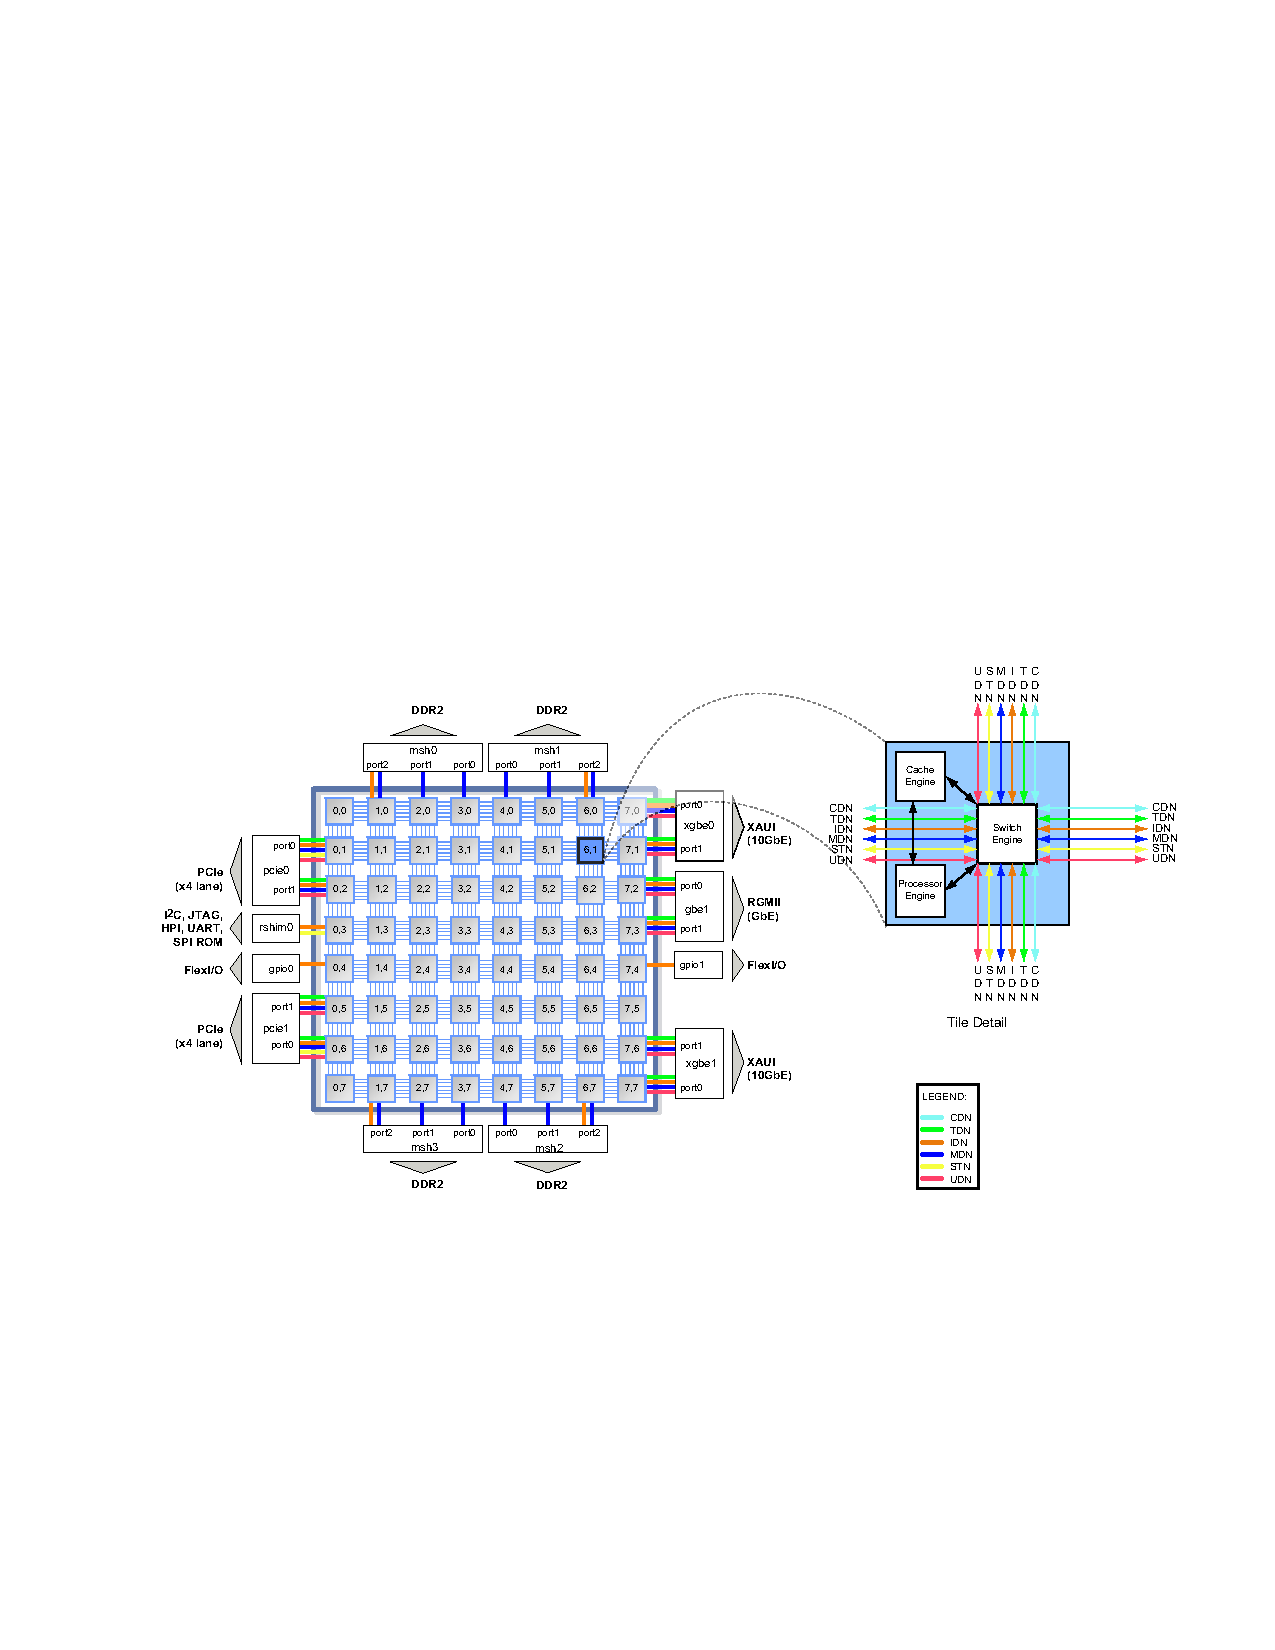
\includegraphics{TilePro64_schema.pdf}}
    \column{.5\textwidth} 
    \resizebox{\columnwidth}{!}{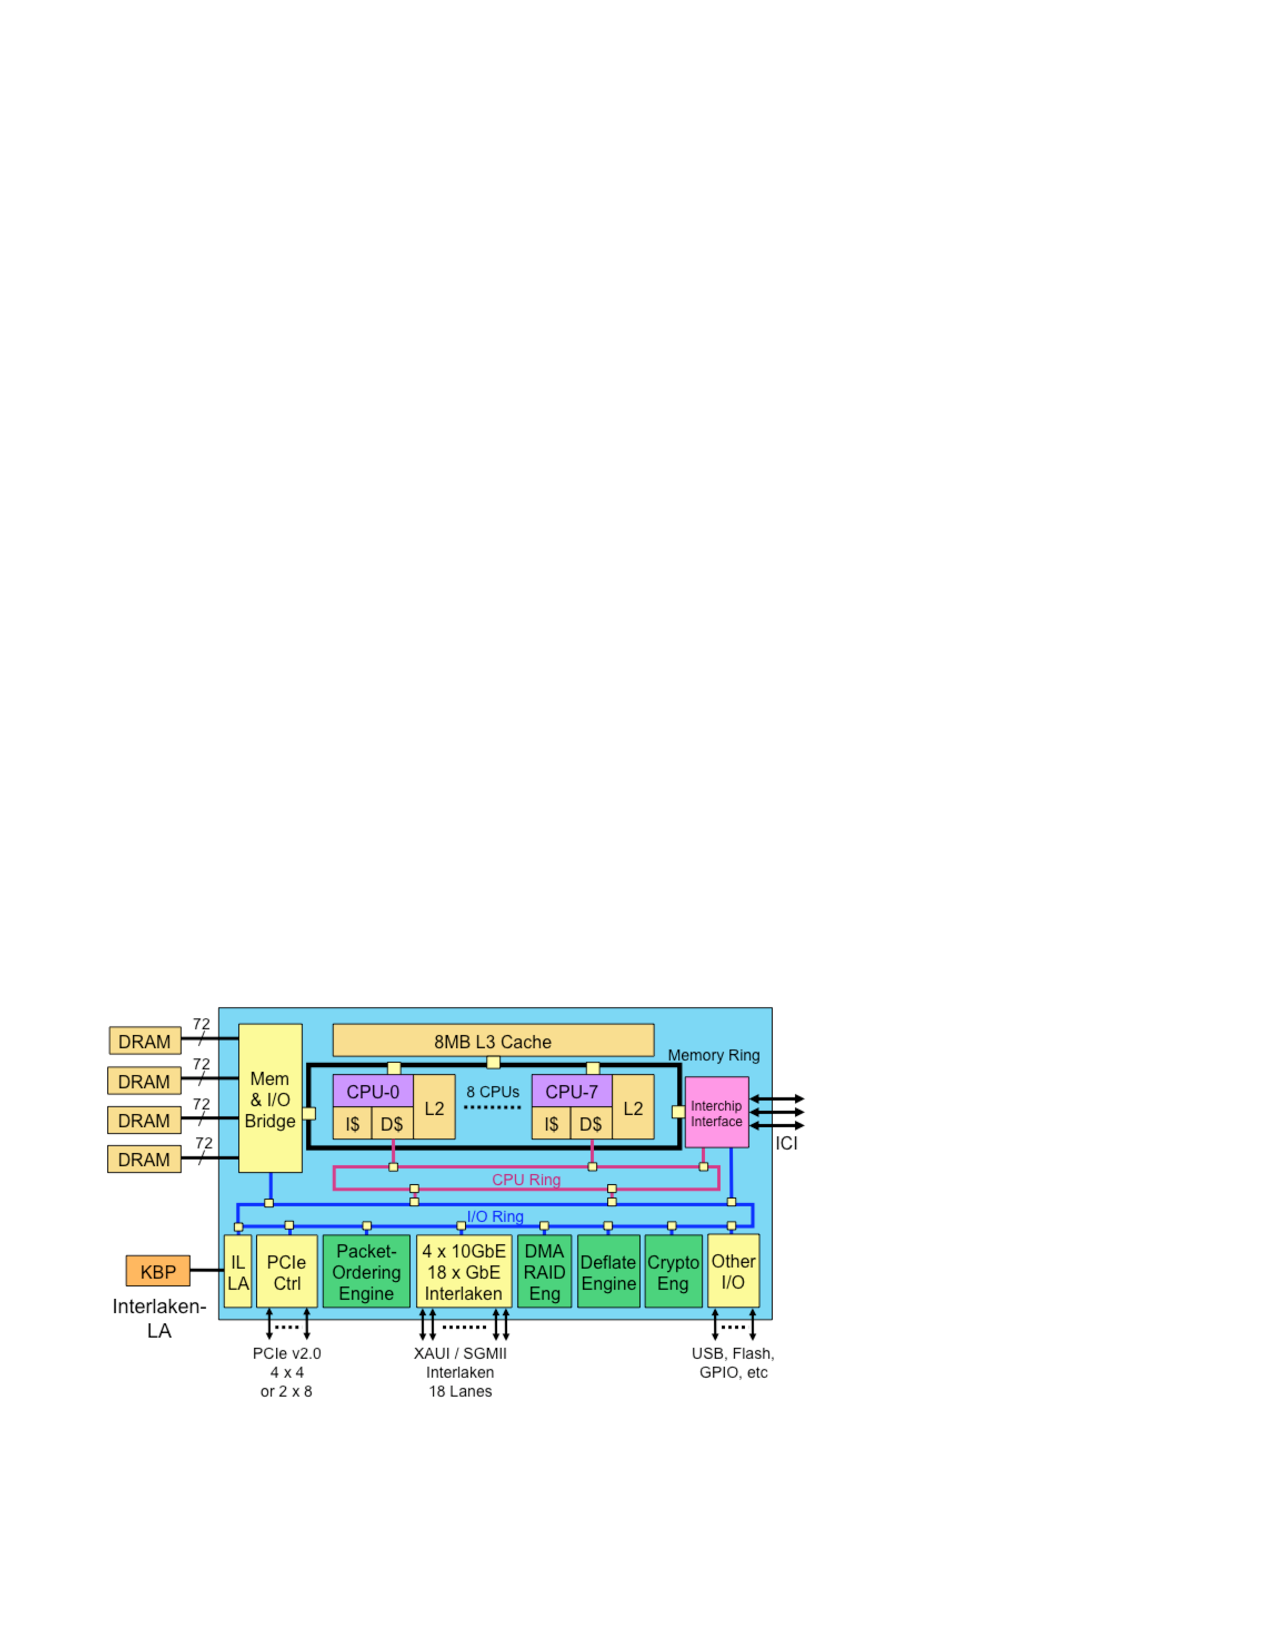
\includegraphics{NetLogic_schema.pdf}}
  \end{columns}
\end{frame}

\section{Supporto alle forme di comunicazione}

\begin{frame}
  \frametitle{Esempi di forme di comunicazione}
  \framesubtitle{Computazioni Data Stream Processing}
  \begin{figure}
    \resizebox{\columnwidth}{!}{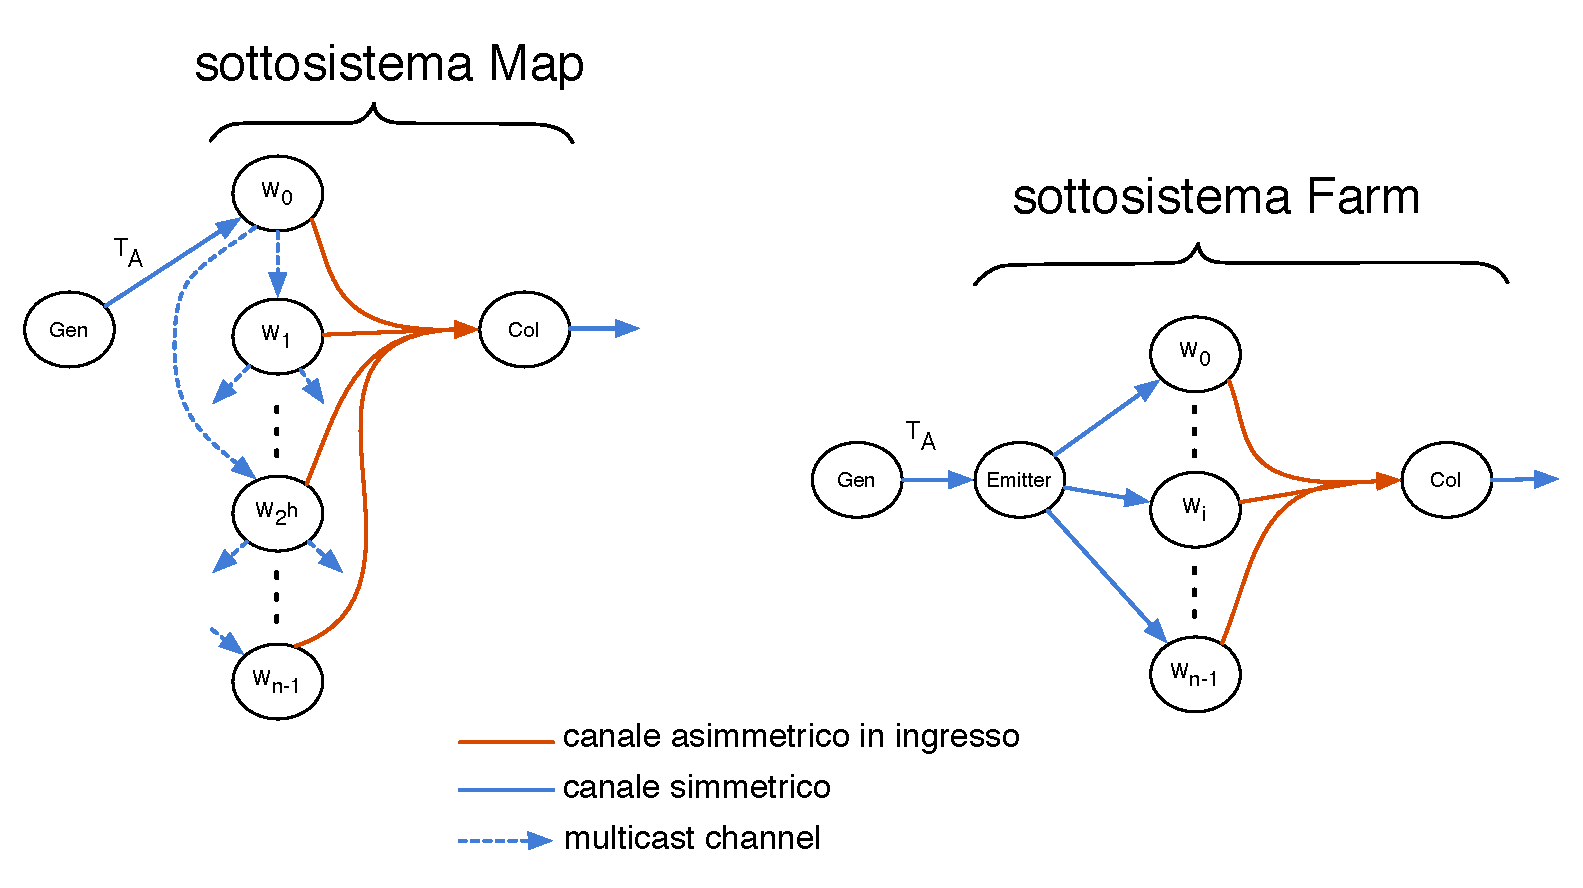
\includegraphics{slide_es_computParall.pdf}}
  \end{figure}
\end{frame}

\begin{frame}
  \frametitle{Reti di interconnessione del Tilera \tile}
  \begin{figure}
    \resizebox{\columnwidth}{!}{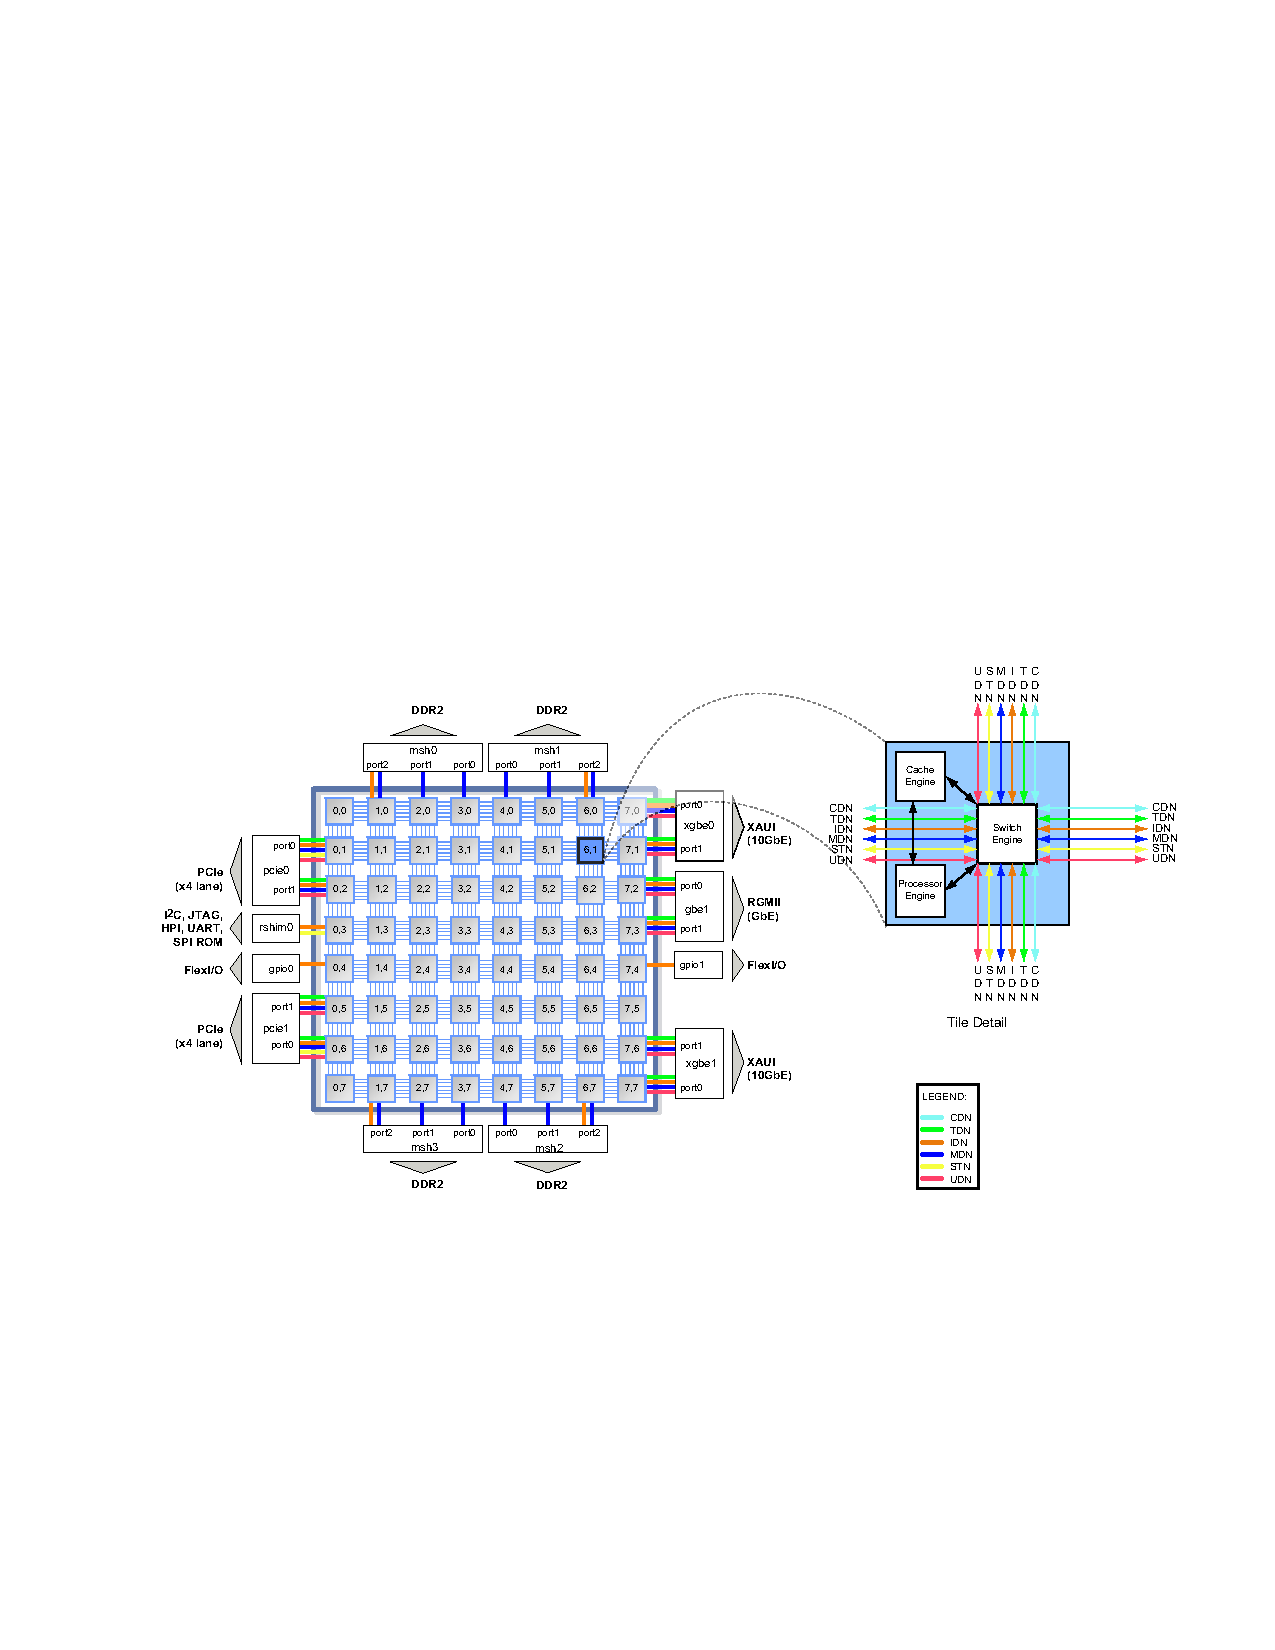
\includegraphics{TilePro64_schema.pdf}}
  \end{figure}
\end{frame}

%% \begin{frame}
%%   \frametitle{Dominio Applicativo}
%%    Computazioni con calcolo di grana fine:
%%     \begin{description}
%%     \item [Data Stream Processing] uno o pi\`u flussi contigui, rapidi e varianti nel tempo di dati; l'elaborazione sui dati in ingresso \`e fatta on-line:\hfill
%%       \begin{itemize}
%%       \item Monitoraggio e sicurezza di reti informatiche;
%%       \item Applicazioni finanziarie;
%%       \item Monitoraggio di sensori e Gestione delle emergenze;
%%       \item Altri \ldots
%%       \end{itemize}
%%     \item [Data Parallel] forma di parallelismo applicabile sia a computazioni su stream che su dato singolo; \`e caratterizzata dal partizionamento dei dati.
%%       \begin{itemize}
%%       \item le comunicazioni sono presenti nella realizzazione delle comunicazioni collettive e se esistono per le dipendenze sui dati (forme \emph{Stencil})
%%       \end{itemize}
%%     \end{description}
%% \end{frame}

\begin{frame}
  \frametitle{I due approcci realizzativi del supporto alle comunicazioni}
  \begin{center}
    \begin{tabular}{cc}
      \tiny Utilizzo della Rete di Interconnessione \scriptsize UDN &
      \tiny Utilizzo della Memoria Condivisa \\
      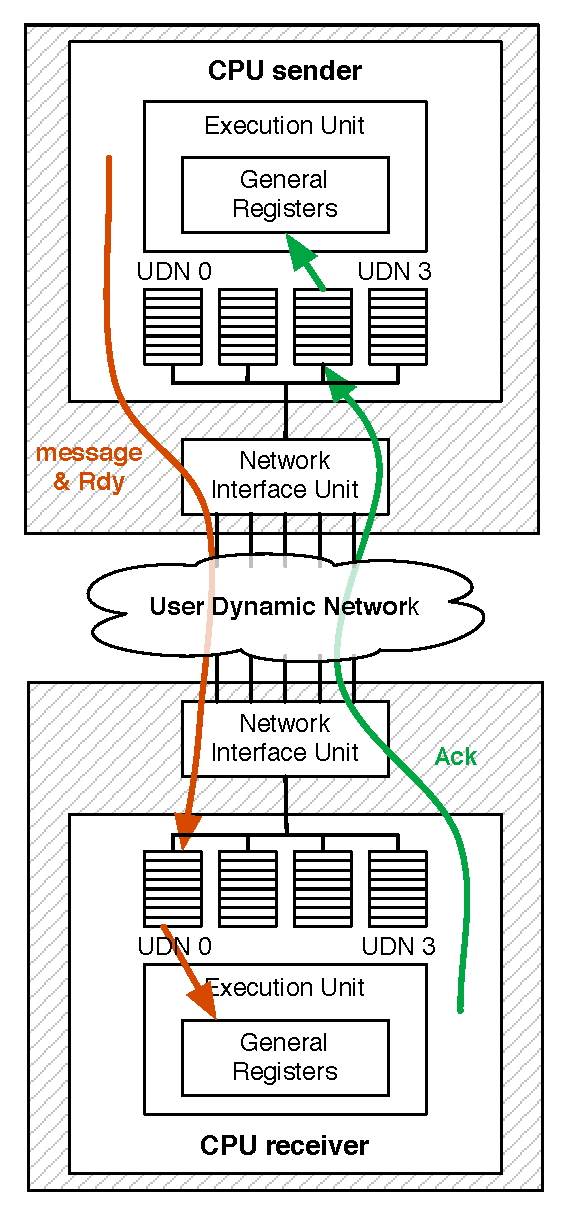
\includegraphics[height=2.7in]{schema_udn_demuxqueue.pdf} &
      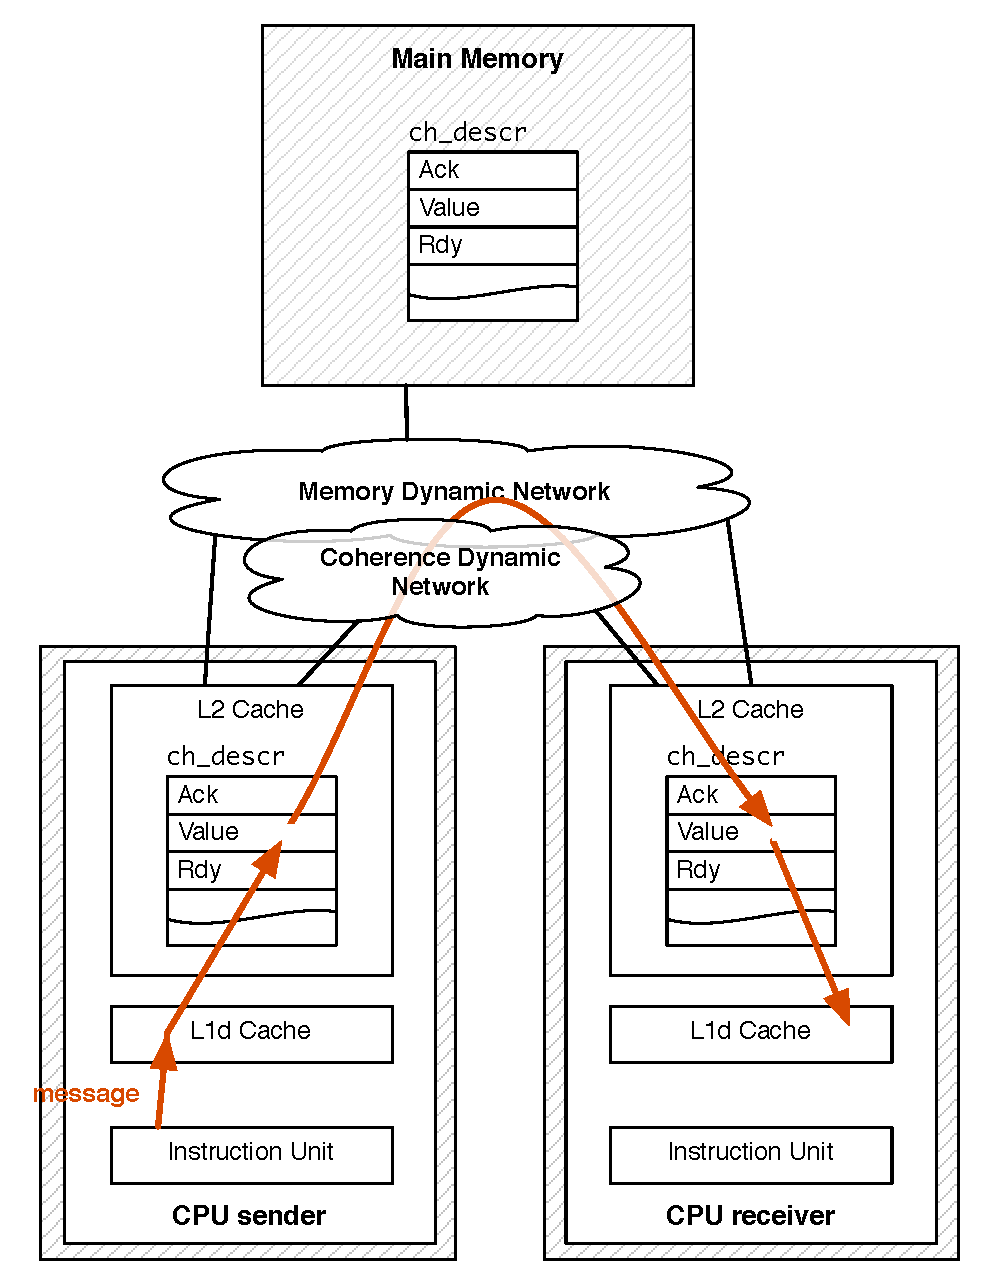
\includegraphics[height=2.7in]{schema_sm.pdf}
    \end{tabular}
  \end{center}
\end{frame}

\section{Esperimenti}

\subsection{Misura della Latenza di comunicazione}

\begin{frame}
  \frametitle{Misura della latenza di comunicazione}
  \begin{itemize}
  \item La latenza di comunicazione \`e misurata per mezzo di una applicazione ``ping-pong'':
    \begin{itemize}
    \item composta da due processi collegati da due canali,
    \item viene svolto lo scambio di $m$ messaggi tra i due processi;
    \end{itemize}
  \item La latenza di comunicazione \`e stimata con $\Lcom = \Tc / (2 \cdot m)$.
  \end{itemize}
  \begin{figure}
    \resizebox{\columnwidth}{!}{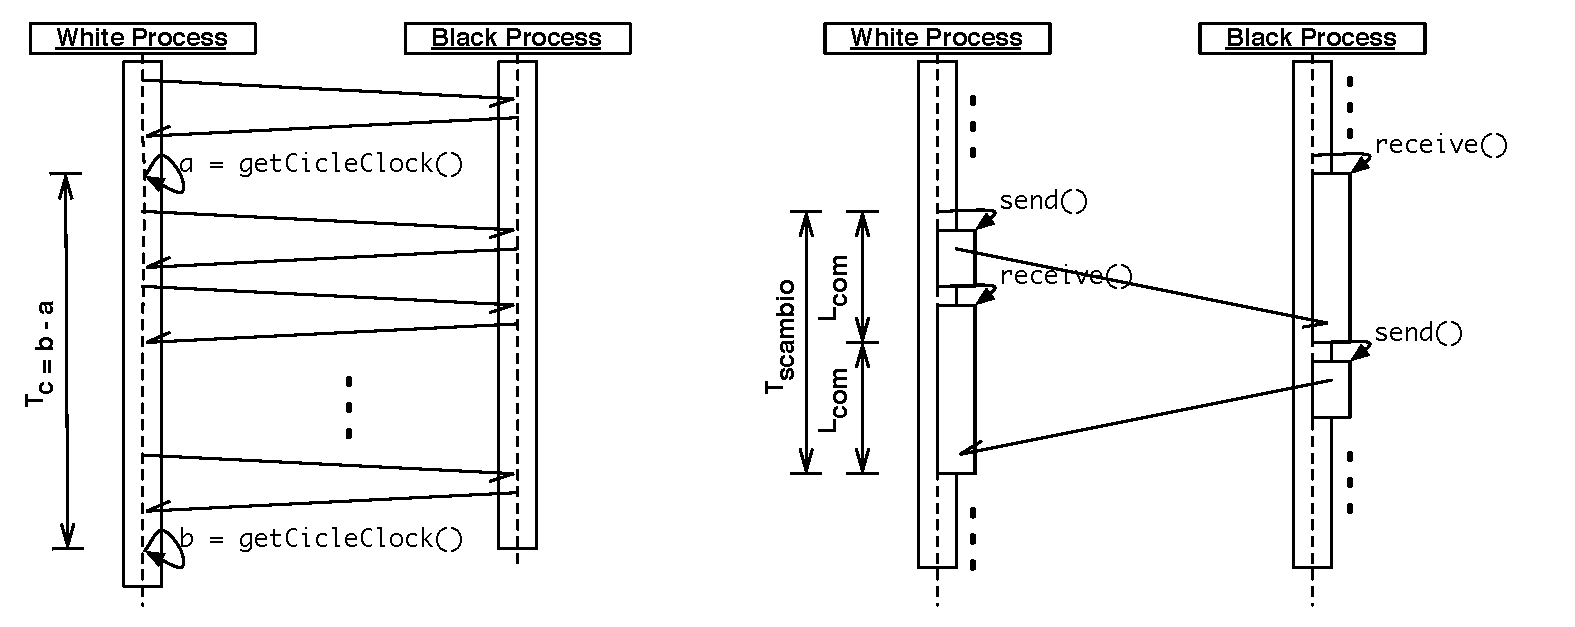
\includegraphics{schema_metering.pdf}}
  \end{figure}
\end{frame}

\begin{frame}
  \frametitle{Misura della latenza del canale simmetrico}
  \begin{figure}
    \resizebox{!}{2.7in}{% GNUPLOT: LaTeX picture with Postscript
\begingroup
  \makeatletter
  \providecommand\color[2][]{%
    \GenericError{(gnuplot) \space\space\space\@spaces}{%
      Package color not loaded in conjunction with
      terminal option `colourtext'%
    }{See the gnuplot documentation for explanation.%
    }{Either use 'blacktext' in gnuplot or load the package
      color.sty in LaTeX.}%
    \renewcommand\color[2][]{}%
  }%
  \providecommand\includegraphics[2][]{%
    \GenericError{(gnuplot) \space\space\space\@spaces}{%
      Package graphicx or graphics not loaded%
    }{See the gnuplot documentation for explanation.%
    }{The gnuplot epslatex terminal needs graphicx.sty or graphics.sty.}%
    \renewcommand\includegraphics[2][]{}%
  }%
  \providecommand\rotatebox[2]{#2}%
  \@ifundefined{ifGPcolor}{%
    \newif\ifGPcolor
    \GPcolortrue
  }{}%
  \@ifundefined{ifGPblacktext}{%
    \newif\ifGPblacktext
    \GPblacktexttrue
  }{}%
  % define a \g@addto@macro without @ in the name:
  \let\gplgaddtomacro\g@addto@macro
  % define empty templates for all commands taking text:
  \gdef\gplbacktext{}%
  \gdef\gplfronttext{}%
  \makeatother
  \ifGPblacktext
    % no textcolor at all
    \def\colorrgb#1{}%
    \def\colorgray#1{}%
  \else
    % gray or color?
    \ifGPcolor
      \def\colorrgb#1{\color[rgb]{#1}}%
      \def\colorgray#1{\color[gray]{#1}}%
      \expandafter\def\csname LTw\endcsname{\color{white}}%
      \expandafter\def\csname LTb\endcsname{\color{black}}%
      \expandafter\def\csname LTa\endcsname{\color{black}}%
      \expandafter\def\csname LT0\endcsname{\color[rgb]{1,0,0}}%
      \expandafter\def\csname LT1\endcsname{\color[rgb]{0,1,0}}%
      \expandafter\def\csname LT2\endcsname{\color[rgb]{0,0,1}}%
      \expandafter\def\csname LT3\endcsname{\color[rgb]{1,0,1}}%
      \expandafter\def\csname LT4\endcsname{\color[rgb]{0,1,1}}%
      \expandafter\def\csname LT5\endcsname{\color[rgb]{1,1,0}}%
      \expandafter\def\csname LT6\endcsname{\color[rgb]{0,0,0}}%
      \expandafter\def\csname LT7\endcsname{\color[rgb]{1,0.3,0}}%
      \expandafter\def\csname LT8\endcsname{\color[rgb]{0.5,0.5,0.5}}%
    \else
      % gray
      \def\colorrgb#1{\color{black}}%
      \def\colorgray#1{\color[gray]{#1}}%
      \expandafter\def\csname LTw\endcsname{\color{white}}%
      \expandafter\def\csname LTb\endcsname{\color{black}}%
      \expandafter\def\csname LTa\endcsname{\color{black}}%
      \expandafter\def\csname LT0\endcsname{\color{black}}%
      \expandafter\def\csname LT1\endcsname{\color{black}}%
      \expandafter\def\csname LT2\endcsname{\color{black}}%
      \expandafter\def\csname LT3\endcsname{\color{black}}%
      \expandafter\def\csname LT4\endcsname{\color{black}}%
      \expandafter\def\csname LT5\endcsname{\color{black}}%
      \expandafter\def\csname LT6\endcsname{\color{black}}%
      \expandafter\def\csname LT7\endcsname{\color{black}}%
      \expandafter\def\csname LT8\endcsname{\color{black}}%
    \fi
  \fi
  \setlength{\unitlength}{0.0500bp}%
  \begin{picture}(7200.00,5040.00)%
    \gplgaddtomacro\gplbacktext{%
      \csname LTb\endcsname%
      \put(946,704){\makebox(0,0)[r]{\strut{} 0}}%
      \put(946,1128){\makebox(0,0)[r]{\strut{} 50}}%
      \put(946,1553){\makebox(0,0)[r]{\strut{} 100}}%
      \put(946,1977){\makebox(0,0)[r]{\strut{} 150}}%
      \put(946,2402){\makebox(0,0)[r]{\strut{} 200}}%
      \put(946,2826){\makebox(0,0)[r]{\strut{} 250}}%
      \put(946,3251){\makebox(0,0)[r]{\strut{} 300}}%
      \put(946,3675){\makebox(0,0)[r]{\strut{} 350}}%
      \put(2223,484){\makebox(0,0){\strut{}1}}%
      \put(3369,484){\makebox(0,0){\strut{}8}}%
      \put(4514,484){\makebox(0,0){\strut{}14}}%
      \put(5791,704){\makebox(0,0)[l]{\strut{} 0}}%
      \put(5791,1071){\makebox(0,0)[l]{\strut{} 0.05}}%
      \put(5791,1438){\makebox(0,0)[l]{\strut{} 0.1}}%
      \put(5791,1805){\makebox(0,0)[l]{\strut{} 0.15}}%
      \put(5791,2172){\makebox(0,0)[l]{\strut{} 0.2}}%
      \put(5791,2539){\makebox(0,0)[l]{\strut{} 0.25}}%
      \put(5791,2906){\makebox(0,0)[l]{\strut{} 0.3}}%
      \put(5791,3273){\makebox(0,0)[l]{\strut{} 0.35}}%
      \put(5791,3640){\makebox(0,0)[l]{\strut{} 0.4}}%
      \put(176,2189){\rotatebox{-270}{\makebox(0,0){\strut{}$\mathrm{L}_{\mathrm{com}} \; (\,\tau\,)$}}}%
      \put(6692,2189){\rotatebox{-270}{\makebox(0,0){\strut{}$\mathrm{L}_{\mathrm{com}} \; (\,\mu\mathrm{sec}\,)$}}}%
      \put(3368,154){\makebox(0,0){\strut{}number of hops}}%
    }%
    \gplgaddtomacro\gplfronttext{%
      \csname LTb\endcsname%
      \put(4804,4867){\makebox(0,0)[r]{\strut{}uso della Rete di Interconnessione}}%
      \csname LTb\endcsname%
      \put(4804,4647){\makebox(0,0)[r]{\strut{}uso della Memoria Condivisa, coerenza cache predefinita}}%
      \csname LTb\endcsname%
      \put(4804,4427){\makebox(0,0)[r]{\strut{}uso della SM, configurazione coerenza cache}}%
      \csname LTb\endcsname%
      \put(4804,4207){\makebox(0,0)[r]{\strut{}uso della Memoria Condivisa, non uso di memory barrier}}%
    }%
    \gplbacktext
    \put(0,0){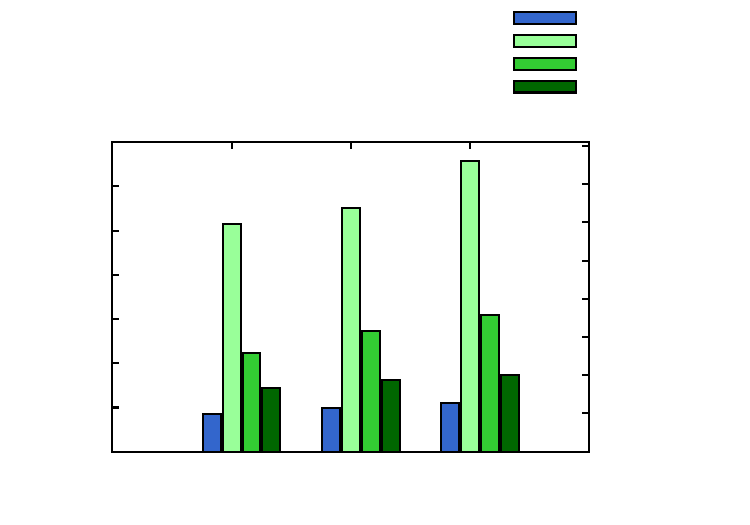
\includegraphics{2_5_sym_all_color}}%
    \gplfronttext
  \end{picture}%
\endgroup
}
  \end{figure}
\end{frame}

\begin{frame}
  \frametitle{Misura della latenza del canale asimmetrico}
  \begin{figure}
    \resizebox{!}{2.7in}{% GNUPLOT: LaTeX picture with Postscript
\begingroup
  \makeatletter
  \providecommand\color[2][]{%
    \GenericError{(gnuplot) \space\space\space\@spaces}{%
      Package color not loaded in conjunction with
      terminal option `colourtext'%
    }{See the gnuplot documentation for explanation.%
    }{Either use 'blacktext' in gnuplot or load the package
      color.sty in LaTeX.}%
    \renewcommand\color[2][]{}%
  }%
  \providecommand\includegraphics[2][]{%
    \GenericError{(gnuplot) \space\space\space\@spaces}{%
      Package graphicx or graphics not loaded%
    }{See the gnuplot documentation for explanation.%
    }{The gnuplot epslatex terminal needs graphicx.sty or graphics.sty.}%
    \renewcommand\includegraphics[2][]{}%
  }%
  \providecommand\rotatebox[2]{#2}%
  \@ifundefined{ifGPcolor}{%
    \newif\ifGPcolor
    \GPcolortrue
  }{}%
  \@ifundefined{ifGPblacktext}{%
    \newif\ifGPblacktext
    \GPblacktexttrue
  }{}%
  % define a \g@addto@macro without @ in the name:
  \let\gplgaddtomacro\g@addto@macro
  % define empty templates for all commands taking text:
  \gdef\gplbacktext{}%
  \gdef\gplfronttext{}%
  \makeatother
  \ifGPblacktext
    % no textcolor at all
    \def\colorrgb#1{}%
    \def\colorgray#1{}%
  \else
    % gray or color?
    \ifGPcolor
      \def\colorrgb#1{\color[rgb]{#1}}%
      \def\colorgray#1{\color[gray]{#1}}%
      \expandafter\def\csname LTw\endcsname{\color{white}}%
      \expandafter\def\csname LTb\endcsname{\color{black}}%
      \expandafter\def\csname LTa\endcsname{\color{black}}%
      \expandafter\def\csname LT0\endcsname{\color[rgb]{1,0,0}}%
      \expandafter\def\csname LT1\endcsname{\color[rgb]{0,1,0}}%
      \expandafter\def\csname LT2\endcsname{\color[rgb]{0,0,1}}%
      \expandafter\def\csname LT3\endcsname{\color[rgb]{1,0,1}}%
      \expandafter\def\csname LT4\endcsname{\color[rgb]{0,1,1}}%
      \expandafter\def\csname LT5\endcsname{\color[rgb]{1,1,0}}%
      \expandafter\def\csname LT6\endcsname{\color[rgb]{0,0,0}}%
      \expandafter\def\csname LT7\endcsname{\color[rgb]{1,0.3,0}}%
      \expandafter\def\csname LT8\endcsname{\color[rgb]{0.5,0.5,0.5}}%
    \else
      % gray
      \def\colorrgb#1{\color{black}}%
      \def\colorgray#1{\color[gray]{#1}}%
      \expandafter\def\csname LTw\endcsname{\color{white}}%
      \expandafter\def\csname LTb\endcsname{\color{black}}%
      \expandafter\def\csname LTa\endcsname{\color{black}}%
      \expandafter\def\csname LT0\endcsname{\color{black}}%
      \expandafter\def\csname LT1\endcsname{\color{black}}%
      \expandafter\def\csname LT2\endcsname{\color{black}}%
      \expandafter\def\csname LT3\endcsname{\color{black}}%
      \expandafter\def\csname LT4\endcsname{\color{black}}%
      \expandafter\def\csname LT5\endcsname{\color{black}}%
      \expandafter\def\csname LT6\endcsname{\color{black}}%
      \expandafter\def\csname LT7\endcsname{\color{black}}%
      \expandafter\def\csname LT8\endcsname{\color{black}}%
    \fi
  \fi
  \setlength{\unitlength}{0.0500bp}%
  \begin{picture}(7200.00,5040.00)%
    \gplgaddtomacro\gplbacktext{%
      \csname LTb\endcsname%
      \put(946,704){\makebox(0,0)[r]{\strut{} 0}}%
      \put(946,1059){\makebox(0,0)[r]{\strut{} 50}}%
      \put(946,1413){\makebox(0,0)[r]{\strut{} 100}}%
      \put(946,1768){\makebox(0,0)[r]{\strut{} 150}}%
      \put(946,2122){\makebox(0,0)[r]{\strut{} 200}}%
      \put(946,2477){\makebox(0,0)[r]{\strut{} 250}}%
      \put(946,2831){\makebox(0,0)[r]{\strut{} 300}}%
      \put(946,3186){\makebox(0,0)[r]{\strut{} 350}}%
      \put(946,3540){\makebox(0,0)[r]{\strut{} 400}}%
      \put(946,3895){\makebox(0,0)[r]{\strut{} 450}}%
      \put(2256,484){\makebox(0,0){\strut{}1}}%
      \put(3435,484){\makebox(0,0){\strut{}8}}%
      \put(4613,484){\makebox(0,0){\strut{}14}}%
      \put(5923,704){\makebox(0,0)[l]{\strut{} 0}}%
      \put(5923,1317){\makebox(0,0)[l]{\strut{} 0.1}}%
      \put(5923,1930){\makebox(0,0)[l]{\strut{} 0.2}}%
      \put(5923,2543){\makebox(0,0)[l]{\strut{} 0.3}}%
      \put(5923,3156){\makebox(0,0)[l]{\strut{} 0.4}}%
      \put(5923,3769){\makebox(0,0)[l]{\strut{} 0.5}}%
      \put(176,2299){\rotatebox{-270}{\makebox(0,0){\strut{}$\mathrm{L}_{\mathrm{com}} \; (\,\tau\,)$}}}%
      \put(6692,2299){\rotatebox{-270}{\makebox(0,0){\strut{}$\mathrm{L}_{\mathrm{com}} \; (\,\mu\mathrm{sec}\,)$}}}%
      \put(3434,154){\makebox(0,0){\strut{}number of hops}}%
    }%
    \gplgaddtomacro\gplfronttext{%
      \csname LTb\endcsname%
      \put(4936,4867){\makebox(0,0)[r]{\strut{}uso della Rete di Interconnessione}}%
      \csname LTb\endcsname%
      \put(4936,4647){\makebox(0,0)[r]{\strut{}uso della memoria condivisa, allocati tutti i mittenti}}%
      \csname LTb\endcsname%
      \put(4936,4427){\makebox(0,0)[r]{\strut{}uso della memoria condivisa, allocato un unico mittente}}%
    }%
    \gplbacktext
    \put(0,0){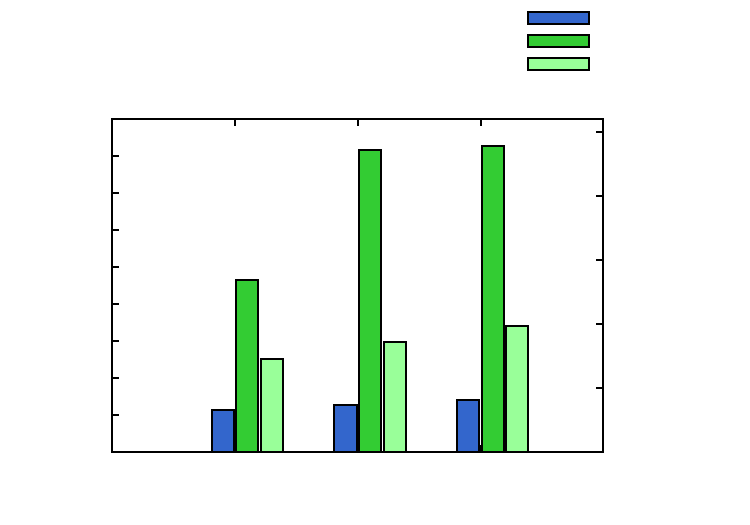
\includegraphics{2_5_asymin_all_color}}%
    \gplfronttext
  \end{picture}%
\endgroup
}
  \end{figure}
\end{frame}

\subsection{Benchmark}

\begin{frame}
  \frametitle{Benchmark: Prodotto matrice-vettore}
  \begin{columns}[c]
  \column{.5\textwidth}
  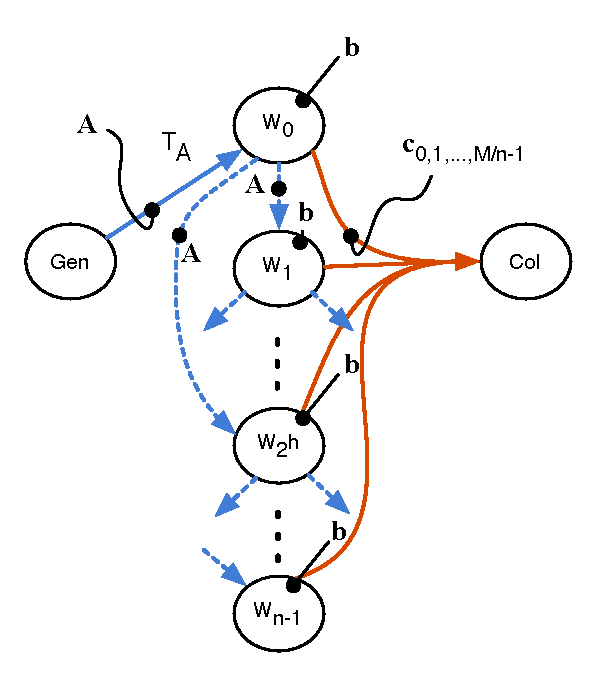
\includegraphics[height=2.9in]{grafo_sigma_slide.pdf}
  \column{.5\textwidth}
  \begin{itemize}
  \item calcolo sequenziale:\begin{flalign*} & \mathbf{A} \in \mathbb{Z}^{\mathrm{MxM}} \, , \, \mathbf{b}, \mathbf{c} \in \mathbb{Z}^{\mathrm{M}} \\ & \forall \; i \in \{1,\ldots,\mathrm{M}\} \; :  \\ & c_i = \mathbf{a}_i \cdot \mathbf{b} = \sum_{j=1}^{\mathrm{M}} a_{ij} \cdot b_j \end{flalign*}
  \item vettore $\mathbf{b}$ costante, stream di matrici $\mathbf{A}$
  \item partizionamento per righe
  \item computazione multicast-compute-gather
  \end{itemize}
\end{columns}
\end{frame}

%% \begin{frame}
%%   \frametitle{Benchmark: prodotto matrice-vettore su stream}
%%   \begin{flalign*}
%%   \mathbf{A} &= (a_{ij})_{i=1,\ldots,\mathrm{M}, \, j=1,\ldots,\mathrm{M}} \in \mathbb{Z}^{\mathrm{MxM}} \\
%%   \mathbf{b} &= (b_1,\ldots,b_\mathrm{M}) \in \mathbb{Z}^{\mathrm{M}} \\
%%   \mathbf{c} &= (c_1,\ldots,c_\mathrm{M}) = \mathbf{A} \cdot \mathbf{b} \in \mathbb{Z}^{\mathrm{M}} \\
%%   &\forall \; i \in \{1,\ldots,\mathrm{M}\} \; : \; c_i = \mathbf{a}_i \cdot \mathbf{b} = \sum_{j=1}^{\mathrm{M}} a_{ij} \cdot b_j 
%%   \end{flalign*}
%%   \begin{columns}[c]
%%     \column{.5\textwidth}
%%     \begin{figure}
%%       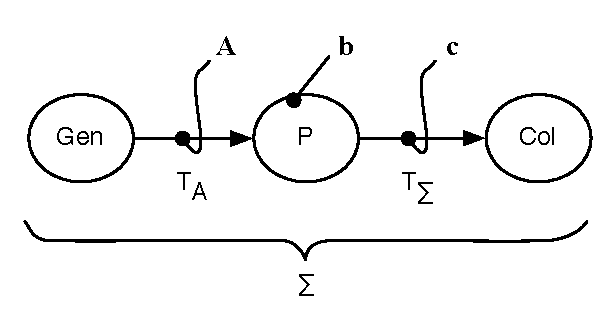
\includegraphics[scale=.5]{grafo_sigma_compatto_slide.pdf}
%%     \end{figure}  
%%     \column{.5\textwidth}
%%     \begin{itemize}
%%     \item computazione su stream di matrici
%%     \item il vettore $\mathbf{b}$ \`e costante per tutta l'esecuzione
%%     \end{itemize}
%%   \end{columns}
  
%% \end{frame}

%% \begin{frame}
%%   \frametitle{Benchmark: soluzione parallela}
%%   \begin{columns}[c]
%%     \column{.5\textwidth}
%%     \begin{itemize}
%% \item Data Parallel Map
%%   \begin{itemize}
%%   \item partizionamento di una matrice per righe
%%   \item replicazione del vettore $\mathbf{b}$ nei processi worker
%%   \end{itemize}
%% \item Multicast strutturata ad albero distribuito nei worker
%% \item $\inTsubsystemId = \; 2 \cdot \inTsymsend + \inTcalc / n + \inTasyminsend$
%% \end{itemize}
%%     \column{.5\textwidth} 
%%   \begin{figure}
%%     \resizebox{!}{\linewidth}{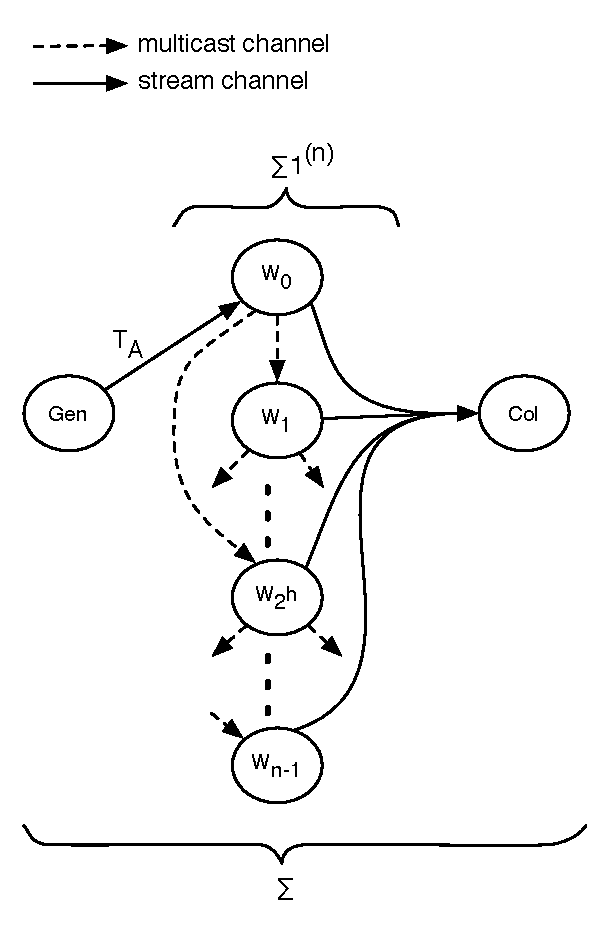
\includegraphics{grafo_sigma_vert.pdf}}
%%   \end{figure}  
%%   \end{columns}
%% \end{frame}

%% \begin{frame}
%%   \frametitle{Confronto: tempo di servizio}
%%   \begin{columns}
%%     \column{.3\columnwidth}
%%     {\small matrice 56x56}
%%     \column{.3\columnwidth}
%%            {\small matrice 168x168}
%%     \column{.3\columnwidth}
%%            {\small matrice 280x280}
%%   \end{columns}
%%   \vspace{5mm}
%%   \begin{columns}
%%     \column{.3\columnwidth}
%%     \resizebox{\columnwidth}{!}{% GNUPLOT: LaTeX picture with Postscript
\begingroup
  \makeatletter
  \providecommand\color[2][]{%
    \GenericError{(gnuplot) \space\space\space\@spaces}{%
      Package color not loaded in conjunction with
      terminal option `colourtext'%
    }{See the gnuplot documentation for explanation.%
    }{Either use 'blacktext' in gnuplot or load the package
      color.sty in LaTeX.}%
    \renewcommand\color[2][]{}%
  }%
  \providecommand\includegraphics[2][]{%
    \GenericError{(gnuplot) \space\space\space\@spaces}{%
      Package graphicx or graphics not loaded%
    }{See the gnuplot documentation for explanation.%
    }{The gnuplot epslatex terminal needs graphicx.sty or graphics.sty.}%
    \renewcommand\includegraphics[2][]{}%
  }%
  \providecommand\rotatebox[2]{#2}%
  \@ifundefined{ifGPcolor}{%
    \newif\ifGPcolor
    \GPcolortrue
  }{}%
  \@ifundefined{ifGPblacktext}{%
    \newif\ifGPblacktext
    \GPblacktexttrue
  }{}%
  % define a \g@addto@macro without @ in the name:
  \let\gplgaddtomacro\g@addto@macro
  % define empty templates for all commands taking text:
  \gdef\gplbacktext{}%
  \gdef\gplfronttext{}%
  \makeatother
  \ifGPblacktext
    % no textcolor at all
    \def\colorrgb#1{}%
    \def\colorgray#1{}%
  \else
    % gray or color?
    \ifGPcolor
      \def\colorrgb#1{\color[rgb]{#1}}%
      \def\colorgray#1{\color[gray]{#1}}%
      \expandafter\def\csname LTw\endcsname{\color{white}}%
      \expandafter\def\csname LTb\endcsname{\color{black}}%
      \expandafter\def\csname LTa\endcsname{\color{black}}%
      \expandafter\def\csname LT0\endcsname{\color[rgb]{1,0,0}}%
      \expandafter\def\csname LT1\endcsname{\color[rgb]{0,1,0}}%
      \expandafter\def\csname LT2\endcsname{\color[rgb]{0,0,1}}%
      \expandafter\def\csname LT3\endcsname{\color[rgb]{1,0,1}}%
      \expandafter\def\csname LT4\endcsname{\color[rgb]{0,1,1}}%
      \expandafter\def\csname LT5\endcsname{\color[rgb]{1,1,0}}%
      \expandafter\def\csname LT6\endcsname{\color[rgb]{0,0,0}}%
      \expandafter\def\csname LT7\endcsname{\color[rgb]{1,0.3,0}}%
      \expandafter\def\csname LT8\endcsname{\color[rgb]{0.5,0.5,0.5}}%
    \else
      % gray
      \def\colorrgb#1{\color{black}}%
      \def\colorgray#1{\color[gray]{#1}}%
      \expandafter\def\csname LTw\endcsname{\color{white}}%
      \expandafter\def\csname LTb\endcsname{\color{black}}%
      \expandafter\def\csname LTa\endcsname{\color{black}}%
      \expandafter\def\csname LT0\endcsname{\color{black}}%
      \expandafter\def\csname LT1\endcsname{\color{black}}%
      \expandafter\def\csname LT2\endcsname{\color{black}}%
      \expandafter\def\csname LT3\endcsname{\color{black}}%
      \expandafter\def\csname LT4\endcsname{\color{black}}%
      \expandafter\def\csname LT5\endcsname{\color{black}}%
      \expandafter\def\csname LT6\endcsname{\color{black}}%
      \expandafter\def\csname LT7\endcsname{\color{black}}%
      \expandafter\def\csname LT8\endcsname{\color{black}}%
    \fi
  \fi
  \setlength{\unitlength}{0.0500bp}%
  \begin{picture}(7200.00,5040.00)%
    \gplgaddtomacro\gplbacktext{%
      \csname LTb\endcsname%
      \put(946,704){\makebox(0,0)[r]{\strut{} 1}}%
      \csname LTb\endcsname%
      \put(946,2740){\makebox(0,0)[r]{\strut{} 10}}%
      \csname LTb\endcsname%
      \put(946,4775){\makebox(0,0)[r]{\strut{} 100}}%
      \csname LTb\endcsname%
      \put(1951,484){\makebox(0,0){\strut{} 10}}%
      \csname LTb\endcsname%
      \put(2922,484){\makebox(0,0){\strut{} 20}}%
      \csname LTb\endcsname%
      \put(3892,484){\makebox(0,0){\strut{} 30}}%
      \csname LTb\endcsname%
      \put(4862,484){\makebox(0,0){\strut{} 40}}%
      \csname LTb\endcsname%
      \put(5833,484){\makebox(0,0){\strut{} 50}}%
      \csname LTb\endcsname%
      \put(6803,484){\makebox(0,0){\strut{} 60}}%
      \put(176,2739){\rotatebox{-270}{\makebox(0,0){\strut{}service time ($\,\mu\mathrm{sec}$\,)}}}%
      \put(3940,154){\makebox(0,0){\strut{}$n$ parallel degree}}%
    }%
    \gplgaddtomacro\gplfronttext{%
      \csname LTb\endcsname%
      \put(5698,4602){\makebox(0,0)[r]{\strut{}uso della Rete di Interconnessione}}%
      \csname LTb\endcsname%
      \put(5698,4382){\makebox(0,0)[r]{\strut{}uso della Memoria Condivisa}}%
    }%
    \gplbacktext
    \put(0,0){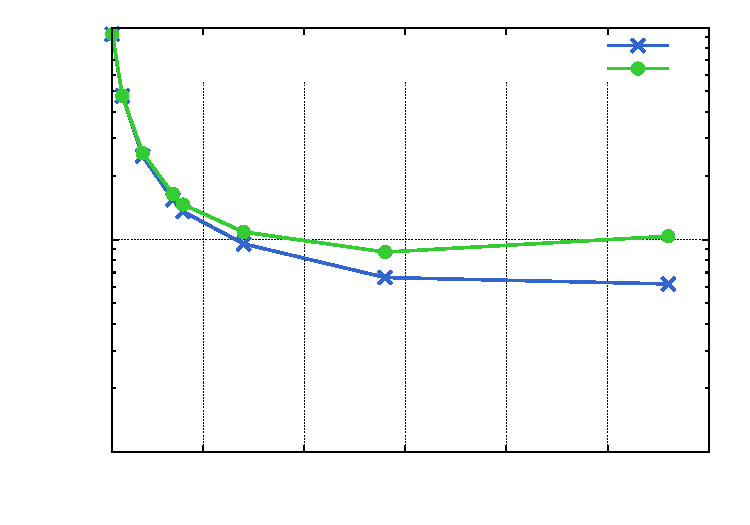
\includegraphics{plot-T-UDN-SM_nogatherInt_selected_500_selected_56_slide_2}}%
    \gplfronttext
  \end{picture}%
\endgroup
}
%%     \column{.3\columnwidth}
%%     \resizebox{\columnwidth}{!}{% GNUPLOT: LaTeX picture with Postscript
\begingroup
  \makeatletter
  \providecommand\color[2][]{%
    \GenericError{(gnuplot) \space\space\space\@spaces}{%
      Package color not loaded in conjunction with
      terminal option `colourtext'%
    }{See the gnuplot documentation for explanation.%
    }{Either use 'blacktext' in gnuplot or load the package
      color.sty in LaTeX.}%
    \renewcommand\color[2][]{}%
  }%
  \providecommand\includegraphics[2][]{%
    \GenericError{(gnuplot) \space\space\space\@spaces}{%
      Package graphicx or graphics not loaded%
    }{See the gnuplot documentation for explanation.%
    }{The gnuplot epslatex terminal needs graphicx.sty or graphics.sty.}%
    \renewcommand\includegraphics[2][]{}%
  }%
  \providecommand\rotatebox[2]{#2}%
  \@ifundefined{ifGPcolor}{%
    \newif\ifGPcolor
    \GPcolortrue
  }{}%
  \@ifundefined{ifGPblacktext}{%
    \newif\ifGPblacktext
    \GPblacktexttrue
  }{}%
  % define a \g@addto@macro without @ in the name:
  \let\gplgaddtomacro\g@addto@macro
  % define empty templates for all commands taking text:
  \gdef\gplbacktext{}%
  \gdef\gplfronttext{}%
  \makeatother
  \ifGPblacktext
    % no textcolor at all
    \def\colorrgb#1{}%
    \def\colorgray#1{}%
  \else
    % gray or color?
    \ifGPcolor
      \def\colorrgb#1{\color[rgb]{#1}}%
      \def\colorgray#1{\color[gray]{#1}}%
      \expandafter\def\csname LTw\endcsname{\color{white}}%
      \expandafter\def\csname LTb\endcsname{\color{black}}%
      \expandafter\def\csname LTa\endcsname{\color{black}}%
      \expandafter\def\csname LT0\endcsname{\color[rgb]{1,0,0}}%
      \expandafter\def\csname LT1\endcsname{\color[rgb]{0,1,0}}%
      \expandafter\def\csname LT2\endcsname{\color[rgb]{0,0,1}}%
      \expandafter\def\csname LT3\endcsname{\color[rgb]{1,0,1}}%
      \expandafter\def\csname LT4\endcsname{\color[rgb]{0,1,1}}%
      \expandafter\def\csname LT5\endcsname{\color[rgb]{1,1,0}}%
      \expandafter\def\csname LT6\endcsname{\color[rgb]{0,0,0}}%
      \expandafter\def\csname LT7\endcsname{\color[rgb]{1,0.3,0}}%
      \expandafter\def\csname LT8\endcsname{\color[rgb]{0.5,0.5,0.5}}%
    \else
      % gray
      \def\colorrgb#1{\color{black}}%
      \def\colorgray#1{\color[gray]{#1}}%
      \expandafter\def\csname LTw\endcsname{\color{white}}%
      \expandafter\def\csname LTb\endcsname{\color{black}}%
      \expandafter\def\csname LTa\endcsname{\color{black}}%
      \expandafter\def\csname LT0\endcsname{\color{black}}%
      \expandafter\def\csname LT1\endcsname{\color{black}}%
      \expandafter\def\csname LT2\endcsname{\color{black}}%
      \expandafter\def\csname LT3\endcsname{\color{black}}%
      \expandafter\def\csname LT4\endcsname{\color{black}}%
      \expandafter\def\csname LT5\endcsname{\color{black}}%
      \expandafter\def\csname LT6\endcsname{\color{black}}%
      \expandafter\def\csname LT7\endcsname{\color{black}}%
      \expandafter\def\csname LT8\endcsname{\color{black}}%
    \fi
  \fi
  \setlength{\unitlength}{0.0500bp}%
  \begin{picture}(7200.00,5040.00)%
    \gplgaddtomacro\gplbacktext{%
      \csname LTb\endcsname%
      \put(1078,704){\makebox(0,0)[r]{\strut{} 10}}%
      \csname LTb\endcsname%
      \put(1078,2740){\makebox(0,0)[r]{\strut{} 100}}%
      \csname LTb\endcsname%
      \put(1078,4775){\makebox(0,0)[r]{\strut{} 1000}}%
      \csname LTb\endcsname%
      \put(2063,484){\makebox(0,0){\strut{} 10}}%
      \csname LTb\endcsname%
      \put(3011,484){\makebox(0,0){\strut{} 20}}%
      \csname LTb\endcsname%
      \put(3959,484){\makebox(0,0){\strut{} 30}}%
      \csname LTb\endcsname%
      \put(4907,484){\makebox(0,0){\strut{} 40}}%
      \csname LTb\endcsname%
      \put(5855,484){\makebox(0,0){\strut{} 50}}%
      \csname LTb\endcsname%
      \put(6803,484){\makebox(0,0){\strut{} 60}}%
      \put(176,2739){\rotatebox{-270}{\makebox(0,0){\strut{}service time ($\,\mu\mathrm{sec}$\,)}}}%
      \put(4006,154){\makebox(0,0){\strut{}$n$ parallel degree}}%
    }%
    \gplgaddtomacro\gplfronttext{%
      \csname LTb\endcsname%
      \put(5830,4602){\makebox(0,0)[r]{\strut{}uso della Rete di Interconnessione}}%
      \csname LTb\endcsname%
      \put(5830,4382){\makebox(0,0)[r]{\strut{}uso della Memoria Condivisa}}%
    }%
    \gplbacktext
    \put(0,0){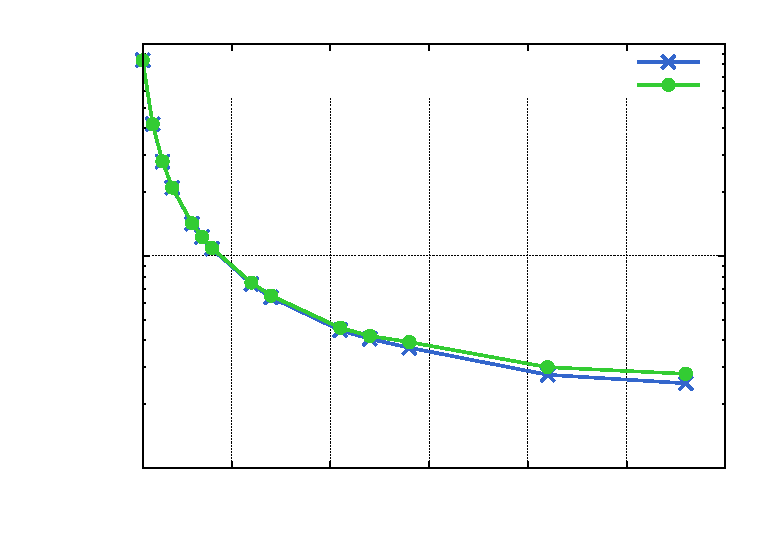
\includegraphics{plot-T-UDN-SM_nogatherInt_selected_500_selected_168_slide_2}}%
    \gplfronttext
  \end{picture}%
\endgroup
}
%%     \column{.3\columnwidth}
%%     \resizebox{\columnwidth}{!}{% GNUPLOT: LaTeX picture with Postscript
\begingroup
  \makeatletter
  \providecommand\color[2][]{%
    \GenericError{(gnuplot) \space\space\space\@spaces}{%
      Package color not loaded in conjunction with
      terminal option `colourtext'%
    }{See the gnuplot documentation for explanation.%
    }{Either use 'blacktext' in gnuplot or load the package
      color.sty in LaTeX.}%
    \renewcommand\color[2][]{}%
  }%
  \providecommand\includegraphics[2][]{%
    \GenericError{(gnuplot) \space\space\space\@spaces}{%
      Package graphicx or graphics not loaded%
    }{See the gnuplot documentation for explanation.%
    }{The gnuplot epslatex terminal needs graphicx.sty or graphics.sty.}%
    \renewcommand\includegraphics[2][]{}%
  }%
  \providecommand\rotatebox[2]{#2}%
  \@ifundefined{ifGPcolor}{%
    \newif\ifGPcolor
    \GPcolortrue
  }{}%
  \@ifundefined{ifGPblacktext}{%
    \newif\ifGPblacktext
    \GPblacktexttrue
  }{}%
  % define a \g@addto@macro without @ in the name:
  \let\gplgaddtomacro\g@addto@macro
  % define empty templates for all commands taking text:
  \gdef\gplbacktext{}%
  \gdef\gplfronttext{}%
  \makeatother
  \ifGPblacktext
    % no textcolor at all
    \def\colorrgb#1{}%
    \def\colorgray#1{}%
  \else
    % gray or color?
    \ifGPcolor
      \def\colorrgb#1{\color[rgb]{#1}}%
      \def\colorgray#1{\color[gray]{#1}}%
      \expandafter\def\csname LTw\endcsname{\color{white}}%
      \expandafter\def\csname LTb\endcsname{\color{black}}%
      \expandafter\def\csname LTa\endcsname{\color{black}}%
      \expandafter\def\csname LT0\endcsname{\color[rgb]{1,0,0}}%
      \expandafter\def\csname LT1\endcsname{\color[rgb]{0,1,0}}%
      \expandafter\def\csname LT2\endcsname{\color[rgb]{0,0,1}}%
      \expandafter\def\csname LT3\endcsname{\color[rgb]{1,0,1}}%
      \expandafter\def\csname LT4\endcsname{\color[rgb]{0,1,1}}%
      \expandafter\def\csname LT5\endcsname{\color[rgb]{1,1,0}}%
      \expandafter\def\csname LT6\endcsname{\color[rgb]{0,0,0}}%
      \expandafter\def\csname LT7\endcsname{\color[rgb]{1,0.3,0}}%
      \expandafter\def\csname LT8\endcsname{\color[rgb]{0.5,0.5,0.5}}%
    \else
      % gray
      \def\colorrgb#1{\color{black}}%
      \def\colorgray#1{\color[gray]{#1}}%
      \expandafter\def\csname LTw\endcsname{\color{white}}%
      \expandafter\def\csname LTb\endcsname{\color{black}}%
      \expandafter\def\csname LTa\endcsname{\color{black}}%
      \expandafter\def\csname LT0\endcsname{\color{black}}%
      \expandafter\def\csname LT1\endcsname{\color{black}}%
      \expandafter\def\csname LT2\endcsname{\color{black}}%
      \expandafter\def\csname LT3\endcsname{\color{black}}%
      \expandafter\def\csname LT4\endcsname{\color{black}}%
      \expandafter\def\csname LT5\endcsname{\color{black}}%
      \expandafter\def\csname LT6\endcsname{\color{black}}%
      \expandafter\def\csname LT7\endcsname{\color{black}}%
      \expandafter\def\csname LT8\endcsname{\color{black}}%
    \fi
  \fi
  \setlength{\unitlength}{0.0500bp}%
  \begin{picture}(7200.00,5040.00)%
    \gplgaddtomacro\gplbacktext{%
      \csname LTb\endcsname%
      \put(1210,704){\makebox(0,0)[r]{\strut{} 10}}%
      \csname LTb\endcsname%
      \put(1210,2061){\makebox(0,0)[r]{\strut{} 100}}%
      \csname LTb\endcsname%
      \put(1210,3418){\makebox(0,0)[r]{\strut{} 1000}}%
      \csname LTb\endcsname%
      \put(1210,4775){\makebox(0,0)[r]{\strut{} 10000}}%
      \csname LTb\endcsname%
      \put(2175,484){\makebox(0,0){\strut{} 10}}%
      \csname LTb\endcsname%
      \put(3101,484){\makebox(0,0){\strut{} 20}}%
      \csname LTb\endcsname%
      \put(4026,484){\makebox(0,0){\strut{} 30}}%
      \csname LTb\endcsname%
      \put(4952,484){\makebox(0,0){\strut{} 40}}%
      \csname LTb\endcsname%
      \put(5877,484){\makebox(0,0){\strut{} 50}}%
      \csname LTb\endcsname%
      \put(6803,484){\makebox(0,0){\strut{} 60}}%
      \put(176,2739){\rotatebox{-270}{\makebox(0,0){\strut{}service time ($\,\mu\mathrm{sec}$\,)}}}%
      \put(4072,154){\makebox(0,0){\strut{}$n$ parallel degree}}%
    }%
    \gplgaddtomacro\gplfronttext{%
      \csname LTb\endcsname%
      \put(5962,4602){\makebox(0,0)[r]{\strut{}uso della Rete di Interconnessione}}%
      \csname LTb\endcsname%
      \put(5962,4382){\makebox(0,0)[r]{\strut{}uso della Memoria Condivisa}}%
    }%
    \gplbacktext
    \put(0,0){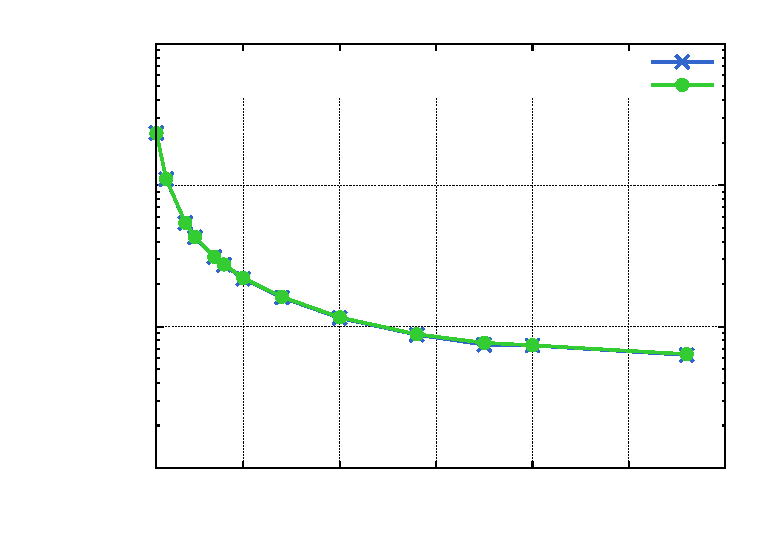
\includegraphics{plot-T-UDN-SM_nogatherInt_selected_500_selected_280_slide_2}}%
    \gplfronttext
  \end{picture}%
\endgroup
}
%%   \end{columns}
%% \end{frame}

%% \begin{frame}
%%   \frametitle{Confronto: tempo di servizio del sottosistema parallelo}
%%   \begin{center}
%%     \begin{tabular}{cc}
%%       \tiny Dimensione delle matrici 56x56 & \tiny Dimensione delle matrici 168x168 \\
%%      \resizebox{!}{1.15in}{% GNUPLOT: LaTeX picture with Postscript
\begingroup
  \makeatletter
  \providecommand\color[2][]{%
    \GenericError{(gnuplot) \space\space\space\@spaces}{%
      Package color not loaded in conjunction with
      terminal option `colourtext'%
    }{See the gnuplot documentation for explanation.%
    }{Either use 'blacktext' in gnuplot or load the package
      color.sty in LaTeX.}%
    \renewcommand\color[2][]{}%
  }%
  \providecommand\includegraphics[2][]{%
    \GenericError{(gnuplot) \space\space\space\@spaces}{%
      Package graphicx or graphics not loaded%
    }{See the gnuplot documentation for explanation.%
    }{The gnuplot epslatex terminal needs graphicx.sty or graphics.sty.}%
    \renewcommand\includegraphics[2][]{}%
  }%
  \providecommand\rotatebox[2]{#2}%
  \@ifundefined{ifGPcolor}{%
    \newif\ifGPcolor
    \GPcolortrue
  }{}%
  \@ifundefined{ifGPblacktext}{%
    \newif\ifGPblacktext
    \GPblacktexttrue
  }{}%
  % define a \g@addto@macro without @ in the name:
  \let\gplgaddtomacro\g@addto@macro
  % define empty templates for all commands taking text:
  \gdef\gplbacktext{}%
  \gdef\gplfronttext{}%
  \makeatother
  \ifGPblacktext
    % no textcolor at all
    \def\colorrgb#1{}%
    \def\colorgray#1{}%
  \else
    % gray or color?
    \ifGPcolor
      \def\colorrgb#1{\color[rgb]{#1}}%
      \def\colorgray#1{\color[gray]{#1}}%
      \expandafter\def\csname LTw\endcsname{\color{white}}%
      \expandafter\def\csname LTb\endcsname{\color{black}}%
      \expandafter\def\csname LTa\endcsname{\color{black}}%
      \expandafter\def\csname LT0\endcsname{\color[rgb]{1,0,0}}%
      \expandafter\def\csname LT1\endcsname{\color[rgb]{0,1,0}}%
      \expandafter\def\csname LT2\endcsname{\color[rgb]{0,0,1}}%
      \expandafter\def\csname LT3\endcsname{\color[rgb]{1,0,1}}%
      \expandafter\def\csname LT4\endcsname{\color[rgb]{0,1,1}}%
      \expandafter\def\csname LT5\endcsname{\color[rgb]{1,1,0}}%
      \expandafter\def\csname LT6\endcsname{\color[rgb]{0,0,0}}%
      \expandafter\def\csname LT7\endcsname{\color[rgb]{1,0.3,0}}%
      \expandafter\def\csname LT8\endcsname{\color[rgb]{0.5,0.5,0.5}}%
    \else
      % gray
      \def\colorrgb#1{\color{black}}%
      \def\colorgray#1{\color[gray]{#1}}%
      \expandafter\def\csname LTw\endcsname{\color{white}}%
      \expandafter\def\csname LTb\endcsname{\color{black}}%
      \expandafter\def\csname LTa\endcsname{\color{black}}%
      \expandafter\def\csname LT0\endcsname{\color{black}}%
      \expandafter\def\csname LT1\endcsname{\color{black}}%
      \expandafter\def\csname LT2\endcsname{\color{black}}%
      \expandafter\def\csname LT3\endcsname{\color{black}}%
      \expandafter\def\csname LT4\endcsname{\color{black}}%
      \expandafter\def\csname LT5\endcsname{\color{black}}%
      \expandafter\def\csname LT6\endcsname{\color{black}}%
      \expandafter\def\csname LT7\endcsname{\color{black}}%
      \expandafter\def\csname LT8\endcsname{\color{black}}%
    \fi
  \fi
  \setlength{\unitlength}{0.0500bp}%
  \begin{picture}(7200.00,5040.00)%
    \gplgaddtomacro\gplbacktext{%
      \csname LTb\endcsname%
      \put(946,704){\makebox(0,0)[r]{\strut{} 1}}%
      \csname LTb\endcsname%
      \put(946,2740){\makebox(0,0)[r]{\strut{} 10}}%
      \csname LTb\endcsname%
      \put(946,4775){\makebox(0,0)[r]{\strut{} 100}}%
      \csname LTb\endcsname%
      \put(1951,484){\makebox(0,0){\strut{} 10}}%
      \csname LTb\endcsname%
      \put(2922,484){\makebox(0,0){\strut{} 20}}%
      \csname LTb\endcsname%
      \put(3892,484){\makebox(0,0){\strut{} 30}}%
      \csname LTb\endcsname%
      \put(4862,484){\makebox(0,0){\strut{} 40}}%
      \csname LTb\endcsname%
      \put(5833,484){\makebox(0,0){\strut{} 50}}%
      \csname LTb\endcsname%
      \put(6803,484){\makebox(0,0){\strut{} 60}}%
      \put(176,2739){\rotatebox{-270}{\makebox(0,0){\strut{}service time ($\,\mu\mathrm{sec}$\,)}}}%
      \put(3940,154){\makebox(0,0){\strut{}$n$ parallel degree}}%
    }%
    \gplgaddtomacro\gplfronttext{%
      \csname LTb\endcsname%
      \put(5698,4602){\makebox(0,0)[r]{\strut{}uso della Rete di Interconnessione}}%
      \csname LTb\endcsname%
      \put(5698,4382){\makebox(0,0)[r]{\strut{}uso della Memoria Condivisa}}%
    }%
    \gplbacktext
    \put(0,0){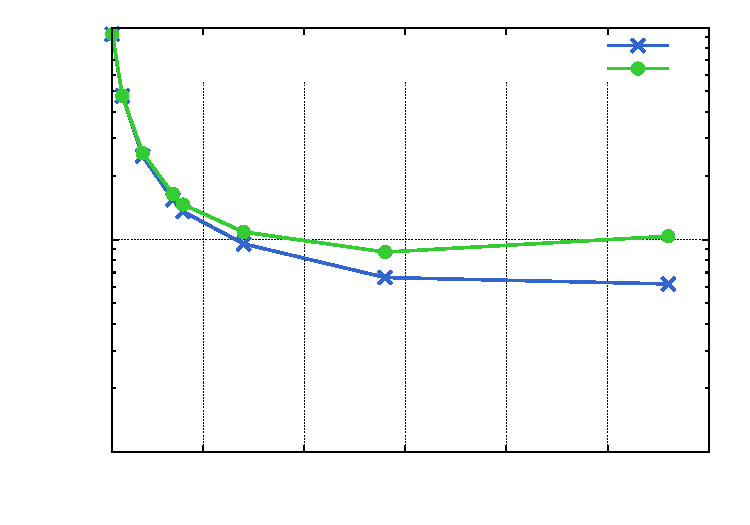
\includegraphics{plot-T-UDN-SM_nogatherInt_selected_500_selected_56_slide_2}}%
    \gplfronttext
  \end{picture}%
\endgroup
}  & \resizebox{!}{1.15in}{% GNUPLOT: LaTeX picture with Postscript
\begingroup
  \makeatletter
  \providecommand\color[2][]{%
    \GenericError{(gnuplot) \space\space\space\@spaces}{%
      Package color not loaded in conjunction with
      terminal option `colourtext'%
    }{See the gnuplot documentation for explanation.%
    }{Either use 'blacktext' in gnuplot or load the package
      color.sty in LaTeX.}%
    \renewcommand\color[2][]{}%
  }%
  \providecommand\includegraphics[2][]{%
    \GenericError{(gnuplot) \space\space\space\@spaces}{%
      Package graphicx or graphics not loaded%
    }{See the gnuplot documentation for explanation.%
    }{The gnuplot epslatex terminal needs graphicx.sty or graphics.sty.}%
    \renewcommand\includegraphics[2][]{}%
  }%
  \providecommand\rotatebox[2]{#2}%
  \@ifundefined{ifGPcolor}{%
    \newif\ifGPcolor
    \GPcolortrue
  }{}%
  \@ifundefined{ifGPblacktext}{%
    \newif\ifGPblacktext
    \GPblacktexttrue
  }{}%
  % define a \g@addto@macro without @ in the name:
  \let\gplgaddtomacro\g@addto@macro
  % define empty templates for all commands taking text:
  \gdef\gplbacktext{}%
  \gdef\gplfronttext{}%
  \makeatother
  \ifGPblacktext
    % no textcolor at all
    \def\colorrgb#1{}%
    \def\colorgray#1{}%
  \else
    % gray or color?
    \ifGPcolor
      \def\colorrgb#1{\color[rgb]{#1}}%
      \def\colorgray#1{\color[gray]{#1}}%
      \expandafter\def\csname LTw\endcsname{\color{white}}%
      \expandafter\def\csname LTb\endcsname{\color{black}}%
      \expandafter\def\csname LTa\endcsname{\color{black}}%
      \expandafter\def\csname LT0\endcsname{\color[rgb]{1,0,0}}%
      \expandafter\def\csname LT1\endcsname{\color[rgb]{0,1,0}}%
      \expandafter\def\csname LT2\endcsname{\color[rgb]{0,0,1}}%
      \expandafter\def\csname LT3\endcsname{\color[rgb]{1,0,1}}%
      \expandafter\def\csname LT4\endcsname{\color[rgb]{0,1,1}}%
      \expandafter\def\csname LT5\endcsname{\color[rgb]{1,1,0}}%
      \expandafter\def\csname LT6\endcsname{\color[rgb]{0,0,0}}%
      \expandafter\def\csname LT7\endcsname{\color[rgb]{1,0.3,0}}%
      \expandafter\def\csname LT8\endcsname{\color[rgb]{0.5,0.5,0.5}}%
    \else
      % gray
      \def\colorrgb#1{\color{black}}%
      \def\colorgray#1{\color[gray]{#1}}%
      \expandafter\def\csname LTw\endcsname{\color{white}}%
      \expandafter\def\csname LTb\endcsname{\color{black}}%
      \expandafter\def\csname LTa\endcsname{\color{black}}%
      \expandafter\def\csname LT0\endcsname{\color{black}}%
      \expandafter\def\csname LT1\endcsname{\color{black}}%
      \expandafter\def\csname LT2\endcsname{\color{black}}%
      \expandafter\def\csname LT3\endcsname{\color{black}}%
      \expandafter\def\csname LT4\endcsname{\color{black}}%
      \expandafter\def\csname LT5\endcsname{\color{black}}%
      \expandafter\def\csname LT6\endcsname{\color{black}}%
      \expandafter\def\csname LT7\endcsname{\color{black}}%
      \expandafter\def\csname LT8\endcsname{\color{black}}%
    \fi
  \fi
  \setlength{\unitlength}{0.0500bp}%
  \begin{picture}(7200.00,5040.00)%
    \gplgaddtomacro\gplbacktext{%
      \csname LTb\endcsname%
      \put(1078,704){\makebox(0,0)[r]{\strut{} 10}}%
      \csname LTb\endcsname%
      \put(1078,2740){\makebox(0,0)[r]{\strut{} 100}}%
      \csname LTb\endcsname%
      \put(1078,4775){\makebox(0,0)[r]{\strut{} 1000}}%
      \csname LTb\endcsname%
      \put(2063,484){\makebox(0,0){\strut{} 10}}%
      \csname LTb\endcsname%
      \put(3011,484){\makebox(0,0){\strut{} 20}}%
      \csname LTb\endcsname%
      \put(3959,484){\makebox(0,0){\strut{} 30}}%
      \csname LTb\endcsname%
      \put(4907,484){\makebox(0,0){\strut{} 40}}%
      \csname LTb\endcsname%
      \put(5855,484){\makebox(0,0){\strut{} 50}}%
      \csname LTb\endcsname%
      \put(6803,484){\makebox(0,0){\strut{} 60}}%
      \put(176,2739){\rotatebox{-270}{\makebox(0,0){\strut{}service time ($\,\mu\mathrm{sec}$\,)}}}%
      \put(4006,154){\makebox(0,0){\strut{}$n$ parallel degree}}%
    }%
    \gplgaddtomacro\gplfronttext{%
      \csname LTb\endcsname%
      \put(5830,4602){\makebox(0,0)[r]{\strut{}uso della Rete di Interconnessione}}%
      \csname LTb\endcsname%
      \put(5830,4382){\makebox(0,0)[r]{\strut{}uso della Memoria Condivisa}}%
    }%
    \gplbacktext
    \put(0,0){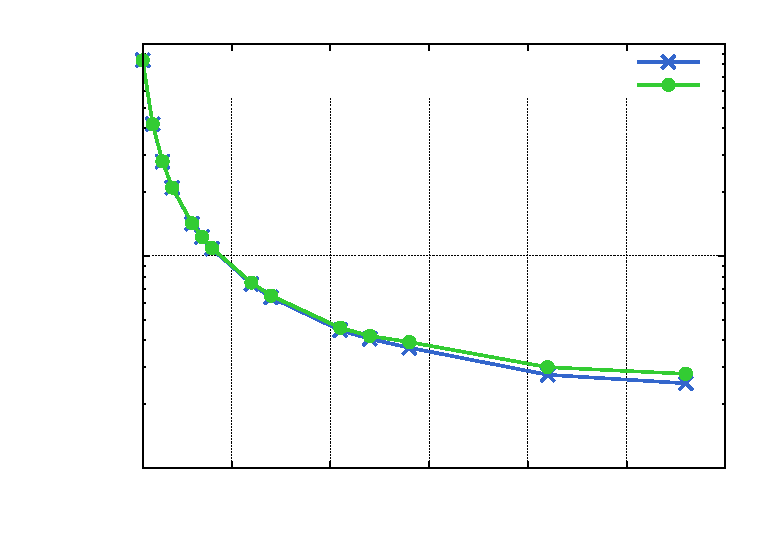
\includegraphics{plot-T-UDN-SM_nogatherInt_selected_500_selected_168_slide_2}}%
    \gplfronttext
  \end{picture}%
\endgroup
} \\
%%      \tiny 2211.562 \musec & \tiny 2349.687 \musec
%%     \end{tabular}
%%   \end{center}
%%   \begin{center}
%%     \begin{tabular}{c}
%%       \tiny Dimensione delle matrici 280x280 \\
%%       \resizebox{!}{1.15in}{% GNUPLOT: LaTeX picture with Postscript
\begingroup
  \makeatletter
  \providecommand\color[2][]{%
    \GenericError{(gnuplot) \space\space\space\@spaces}{%
      Package color not loaded in conjunction with
      terminal option `colourtext'%
    }{See the gnuplot documentation for explanation.%
    }{Either use 'blacktext' in gnuplot or load the package
      color.sty in LaTeX.}%
    \renewcommand\color[2][]{}%
  }%
  \providecommand\includegraphics[2][]{%
    \GenericError{(gnuplot) \space\space\space\@spaces}{%
      Package graphicx or graphics not loaded%
    }{See the gnuplot documentation for explanation.%
    }{The gnuplot epslatex terminal needs graphicx.sty or graphics.sty.}%
    \renewcommand\includegraphics[2][]{}%
  }%
  \providecommand\rotatebox[2]{#2}%
  \@ifundefined{ifGPcolor}{%
    \newif\ifGPcolor
    \GPcolortrue
  }{}%
  \@ifundefined{ifGPblacktext}{%
    \newif\ifGPblacktext
    \GPblacktexttrue
  }{}%
  % define a \g@addto@macro without @ in the name:
  \let\gplgaddtomacro\g@addto@macro
  % define empty templates for all commands taking text:
  \gdef\gplbacktext{}%
  \gdef\gplfronttext{}%
  \makeatother
  \ifGPblacktext
    % no textcolor at all
    \def\colorrgb#1{}%
    \def\colorgray#1{}%
  \else
    % gray or color?
    \ifGPcolor
      \def\colorrgb#1{\color[rgb]{#1}}%
      \def\colorgray#1{\color[gray]{#1}}%
      \expandafter\def\csname LTw\endcsname{\color{white}}%
      \expandafter\def\csname LTb\endcsname{\color{black}}%
      \expandafter\def\csname LTa\endcsname{\color{black}}%
      \expandafter\def\csname LT0\endcsname{\color[rgb]{1,0,0}}%
      \expandafter\def\csname LT1\endcsname{\color[rgb]{0,1,0}}%
      \expandafter\def\csname LT2\endcsname{\color[rgb]{0,0,1}}%
      \expandafter\def\csname LT3\endcsname{\color[rgb]{1,0,1}}%
      \expandafter\def\csname LT4\endcsname{\color[rgb]{0,1,1}}%
      \expandafter\def\csname LT5\endcsname{\color[rgb]{1,1,0}}%
      \expandafter\def\csname LT6\endcsname{\color[rgb]{0,0,0}}%
      \expandafter\def\csname LT7\endcsname{\color[rgb]{1,0.3,0}}%
      \expandafter\def\csname LT8\endcsname{\color[rgb]{0.5,0.5,0.5}}%
    \else
      % gray
      \def\colorrgb#1{\color{black}}%
      \def\colorgray#1{\color[gray]{#1}}%
      \expandafter\def\csname LTw\endcsname{\color{white}}%
      \expandafter\def\csname LTb\endcsname{\color{black}}%
      \expandafter\def\csname LTa\endcsname{\color{black}}%
      \expandafter\def\csname LT0\endcsname{\color{black}}%
      \expandafter\def\csname LT1\endcsname{\color{black}}%
      \expandafter\def\csname LT2\endcsname{\color{black}}%
      \expandafter\def\csname LT3\endcsname{\color{black}}%
      \expandafter\def\csname LT4\endcsname{\color{black}}%
      \expandafter\def\csname LT5\endcsname{\color{black}}%
      \expandafter\def\csname LT6\endcsname{\color{black}}%
      \expandafter\def\csname LT7\endcsname{\color{black}}%
      \expandafter\def\csname LT8\endcsname{\color{black}}%
    \fi
  \fi
  \setlength{\unitlength}{0.0500bp}%
  \begin{picture}(7200.00,5040.00)%
    \gplgaddtomacro\gplbacktext{%
      \csname LTb\endcsname%
      \put(1210,704){\makebox(0,0)[r]{\strut{} 10}}%
      \csname LTb\endcsname%
      \put(1210,2061){\makebox(0,0)[r]{\strut{} 100}}%
      \csname LTb\endcsname%
      \put(1210,3418){\makebox(0,0)[r]{\strut{} 1000}}%
      \csname LTb\endcsname%
      \put(1210,4775){\makebox(0,0)[r]{\strut{} 10000}}%
      \csname LTb\endcsname%
      \put(2175,484){\makebox(0,0){\strut{} 10}}%
      \csname LTb\endcsname%
      \put(3101,484){\makebox(0,0){\strut{} 20}}%
      \csname LTb\endcsname%
      \put(4026,484){\makebox(0,0){\strut{} 30}}%
      \csname LTb\endcsname%
      \put(4952,484){\makebox(0,0){\strut{} 40}}%
      \csname LTb\endcsname%
      \put(5877,484){\makebox(0,0){\strut{} 50}}%
      \csname LTb\endcsname%
      \put(6803,484){\makebox(0,0){\strut{} 60}}%
      \put(176,2739){\rotatebox{-270}{\makebox(0,0){\strut{}service time ($\,\mu\mathrm{sec}$\,)}}}%
      \put(4072,154){\makebox(0,0){\strut{}$n$ parallel degree}}%
    }%
    \gplgaddtomacro\gplfronttext{%
      \csname LTb\endcsname%
      \put(5962,4602){\makebox(0,0)[r]{\strut{}uso della Rete di Interconnessione}}%
      \csname LTb\endcsname%
      \put(5962,4382){\makebox(0,0)[r]{\strut{}uso della Memoria Condivisa}}%
    }%
    \gplbacktext
    \put(0,0){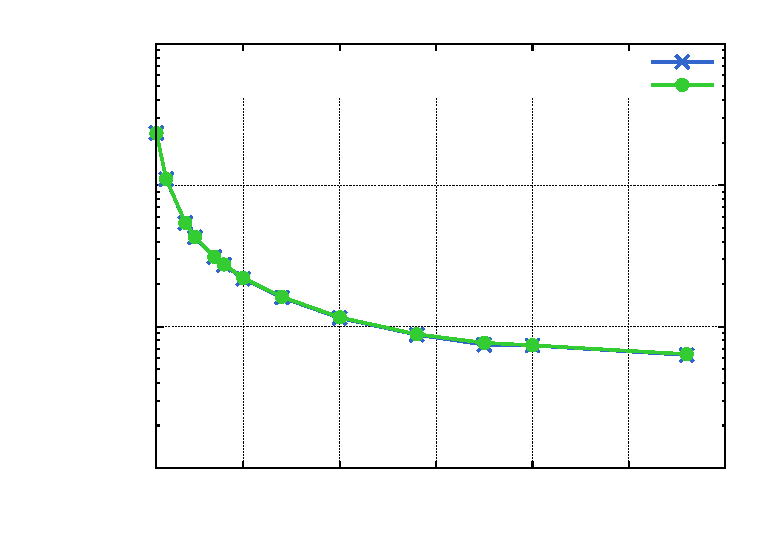
\includegraphics{plot-T-UDN-SM_nogatherInt_selected_500_selected_280_slide_2}}%
    \gplfronttext
  \end{picture}%
\endgroup
} \\
%%       \tiny 821.906
%%     \end{tabular}
%%   \end{center}
%% \end{frame}

\begin{frame}
  \frametitle{Confronto: tempo di servizio del sottosistema parallelo}
  \begin{center}
    \begin{tabular}{cc}
      \tiny Dimensione delle matrici 56x56 & \tiny Dimensione delle matrici 168x168 \\
     \resizebox{!}{1.15in}{% GNUPLOT: LaTeX picture with Postscript
\begingroup
  \makeatletter
  \providecommand\color[2][]{%
    \GenericError{(gnuplot) \space\space\space\@spaces}{%
      Package color not loaded in conjunction with
      terminal option `colourtext'%
    }{See the gnuplot documentation for explanation.%
    }{Either use 'blacktext' in gnuplot or load the package
      color.sty in LaTeX.}%
    \renewcommand\color[2][]{}%
  }%
  \providecommand\includegraphics[2][]{%
    \GenericError{(gnuplot) \space\space\space\@spaces}{%
      Package graphicx or graphics not loaded%
    }{See the gnuplot documentation for explanation.%
    }{The gnuplot epslatex terminal needs graphicx.sty or graphics.sty.}%
    \renewcommand\includegraphics[2][]{}%
  }%
  \providecommand\rotatebox[2]{#2}%
  \@ifundefined{ifGPcolor}{%
    \newif\ifGPcolor
    \GPcolortrue
  }{}%
  \@ifundefined{ifGPblacktext}{%
    \newif\ifGPblacktext
    \GPblacktexttrue
  }{}%
  % define a \g@addto@macro without @ in the name:
  \let\gplgaddtomacro\g@addto@macro
  % define empty templates for all commands taking text:
  \gdef\gplbacktext{}%
  \gdef\gplfronttext{}%
  \makeatother
  \ifGPblacktext
    % no textcolor at all
    \def\colorrgb#1{}%
    \def\colorgray#1{}%
  \else
    % gray or color?
    \ifGPcolor
      \def\colorrgb#1{\color[rgb]{#1}}%
      \def\colorgray#1{\color[gray]{#1}}%
      \expandafter\def\csname LTw\endcsname{\color{white}}%
      \expandafter\def\csname LTb\endcsname{\color{black}}%
      \expandafter\def\csname LTa\endcsname{\color{black}}%
      \expandafter\def\csname LT0\endcsname{\color[rgb]{1,0,0}}%
      \expandafter\def\csname LT1\endcsname{\color[rgb]{0,1,0}}%
      \expandafter\def\csname LT2\endcsname{\color[rgb]{0,0,1}}%
      \expandafter\def\csname LT3\endcsname{\color[rgb]{1,0,1}}%
      \expandafter\def\csname LT4\endcsname{\color[rgb]{0,1,1}}%
      \expandafter\def\csname LT5\endcsname{\color[rgb]{1,1,0}}%
      \expandafter\def\csname LT6\endcsname{\color[rgb]{0,0,0}}%
      \expandafter\def\csname LT7\endcsname{\color[rgb]{1,0.3,0}}%
      \expandafter\def\csname LT8\endcsname{\color[rgb]{0.5,0.5,0.5}}%
    \else
      % gray
      \def\colorrgb#1{\color{black}}%
      \def\colorgray#1{\color[gray]{#1}}%
      \expandafter\def\csname LTw\endcsname{\color{white}}%
      \expandafter\def\csname LTb\endcsname{\color{black}}%
      \expandafter\def\csname LTa\endcsname{\color{black}}%
      \expandafter\def\csname LT0\endcsname{\color{black}}%
      \expandafter\def\csname LT1\endcsname{\color{black}}%
      \expandafter\def\csname LT2\endcsname{\color{black}}%
      \expandafter\def\csname LT3\endcsname{\color{black}}%
      \expandafter\def\csname LT4\endcsname{\color{black}}%
      \expandafter\def\csname LT5\endcsname{\color{black}}%
      \expandafter\def\csname LT6\endcsname{\color{black}}%
      \expandafter\def\csname LT7\endcsname{\color{black}}%
      \expandafter\def\csname LT8\endcsname{\color{black}}%
    \fi
  \fi
  \setlength{\unitlength}{0.0500bp}%
  \begin{picture}(7200.00,5040.00)%
    \gplgaddtomacro\gplbacktext{%
      \csname LTb\endcsname%
      \put(946,704){\makebox(0,0)[r]{\strut{} 1}}%
      \csname LTb\endcsname%
      \put(946,2740){\makebox(0,0)[r]{\strut{} 10}}%
      \csname LTb\endcsname%
      \put(946,4775){\makebox(0,0)[r]{\strut{} 100}}%
      \csname LTb\endcsname%
      \put(1951,484){\makebox(0,0){\strut{} 10}}%
      \csname LTb\endcsname%
      \put(2922,484){\makebox(0,0){\strut{} 20}}%
      \csname LTb\endcsname%
      \put(3892,484){\makebox(0,0){\strut{} 30}}%
      \csname LTb\endcsname%
      \put(4862,484){\makebox(0,0){\strut{} 40}}%
      \csname LTb\endcsname%
      \put(5833,484){\makebox(0,0){\strut{} 50}}%
      \csname LTb\endcsname%
      \put(6803,484){\makebox(0,0){\strut{} 60}}%
      \put(176,2739){\rotatebox{-270}{\makebox(0,0){\strut{}service time ($\,\mu\mathrm{sec}$\,)}}}%
      \put(3940,154){\makebox(0,0){\strut{}$n$ parallel degree}}%
    }%
    \gplgaddtomacro\gplfronttext{%
      \csname LTb\endcsname%
      \put(5698,4602){\makebox(0,0)[r]{\strut{}uso della Rete di Interconnessione}}%
      \csname LTb\endcsname%
      \put(5698,4382){\makebox(0,0)[r]{\strut{}uso della Memoria Condivisa}}%
    }%
    \gplbacktext
    \put(0,0){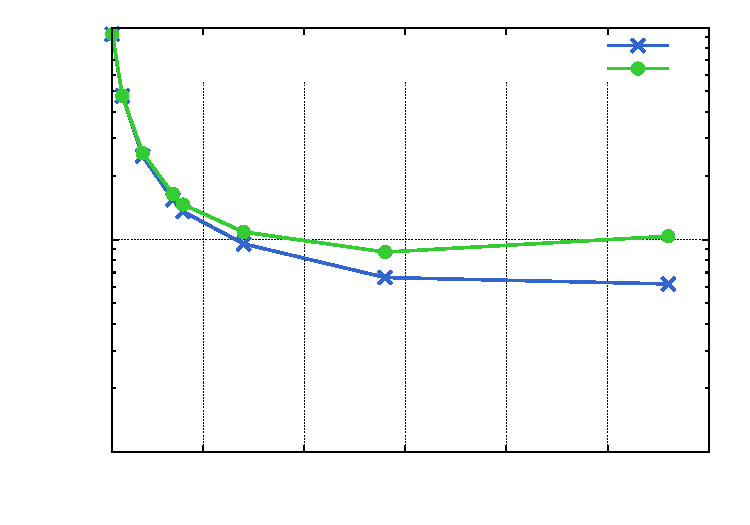
\includegraphics{plot-T-UDN-SM_nogatherInt_selected_500_selected_56_slide_2}}%
    \gplfronttext
  \end{picture}%
\endgroup
}  & \resizebox{!}{1.15in}{% GNUPLOT: LaTeX picture with Postscript
\begingroup
  \makeatletter
  \providecommand\color[2][]{%
    \GenericError{(gnuplot) \space\space\space\@spaces}{%
      Package color not loaded in conjunction with
      terminal option `colourtext'%
    }{See the gnuplot documentation for explanation.%
    }{Either use 'blacktext' in gnuplot or load the package
      color.sty in LaTeX.}%
    \renewcommand\color[2][]{}%
  }%
  \providecommand\includegraphics[2][]{%
    \GenericError{(gnuplot) \space\space\space\@spaces}{%
      Package graphicx or graphics not loaded%
    }{See the gnuplot documentation for explanation.%
    }{The gnuplot epslatex terminal needs graphicx.sty or graphics.sty.}%
    \renewcommand\includegraphics[2][]{}%
  }%
  \providecommand\rotatebox[2]{#2}%
  \@ifundefined{ifGPcolor}{%
    \newif\ifGPcolor
    \GPcolortrue
  }{}%
  \@ifundefined{ifGPblacktext}{%
    \newif\ifGPblacktext
    \GPblacktexttrue
  }{}%
  % define a \g@addto@macro without @ in the name:
  \let\gplgaddtomacro\g@addto@macro
  % define empty templates for all commands taking text:
  \gdef\gplbacktext{}%
  \gdef\gplfronttext{}%
  \makeatother
  \ifGPblacktext
    % no textcolor at all
    \def\colorrgb#1{}%
    \def\colorgray#1{}%
  \else
    % gray or color?
    \ifGPcolor
      \def\colorrgb#1{\color[rgb]{#1}}%
      \def\colorgray#1{\color[gray]{#1}}%
      \expandafter\def\csname LTw\endcsname{\color{white}}%
      \expandafter\def\csname LTb\endcsname{\color{black}}%
      \expandafter\def\csname LTa\endcsname{\color{black}}%
      \expandafter\def\csname LT0\endcsname{\color[rgb]{1,0,0}}%
      \expandafter\def\csname LT1\endcsname{\color[rgb]{0,1,0}}%
      \expandafter\def\csname LT2\endcsname{\color[rgb]{0,0,1}}%
      \expandafter\def\csname LT3\endcsname{\color[rgb]{1,0,1}}%
      \expandafter\def\csname LT4\endcsname{\color[rgb]{0,1,1}}%
      \expandafter\def\csname LT5\endcsname{\color[rgb]{1,1,0}}%
      \expandafter\def\csname LT6\endcsname{\color[rgb]{0,0,0}}%
      \expandafter\def\csname LT7\endcsname{\color[rgb]{1,0.3,0}}%
      \expandafter\def\csname LT8\endcsname{\color[rgb]{0.5,0.5,0.5}}%
    \else
      % gray
      \def\colorrgb#1{\color{black}}%
      \def\colorgray#1{\color[gray]{#1}}%
      \expandafter\def\csname LTw\endcsname{\color{white}}%
      \expandafter\def\csname LTb\endcsname{\color{black}}%
      \expandafter\def\csname LTa\endcsname{\color{black}}%
      \expandafter\def\csname LT0\endcsname{\color{black}}%
      \expandafter\def\csname LT1\endcsname{\color{black}}%
      \expandafter\def\csname LT2\endcsname{\color{black}}%
      \expandafter\def\csname LT3\endcsname{\color{black}}%
      \expandafter\def\csname LT4\endcsname{\color{black}}%
      \expandafter\def\csname LT5\endcsname{\color{black}}%
      \expandafter\def\csname LT6\endcsname{\color{black}}%
      \expandafter\def\csname LT7\endcsname{\color{black}}%
      \expandafter\def\csname LT8\endcsname{\color{black}}%
    \fi
  \fi
  \setlength{\unitlength}{0.0500bp}%
  \begin{picture}(7200.00,5040.00)%
    \gplgaddtomacro\gplbacktext{%
      \csname LTb\endcsname%
      \put(1078,704){\makebox(0,0)[r]{\strut{} 10}}%
      \csname LTb\endcsname%
      \put(1078,2740){\makebox(0,0)[r]{\strut{} 100}}%
      \csname LTb\endcsname%
      \put(1078,4775){\makebox(0,0)[r]{\strut{} 1000}}%
      \csname LTb\endcsname%
      \put(2063,484){\makebox(0,0){\strut{} 10}}%
      \csname LTb\endcsname%
      \put(3011,484){\makebox(0,0){\strut{} 20}}%
      \csname LTb\endcsname%
      \put(3959,484){\makebox(0,0){\strut{} 30}}%
      \csname LTb\endcsname%
      \put(4907,484){\makebox(0,0){\strut{} 40}}%
      \csname LTb\endcsname%
      \put(5855,484){\makebox(0,0){\strut{} 50}}%
      \csname LTb\endcsname%
      \put(6803,484){\makebox(0,0){\strut{} 60}}%
      \put(176,2739){\rotatebox{-270}{\makebox(0,0){\strut{}service time ($\,\mu\mathrm{sec}$\,)}}}%
      \put(4006,154){\makebox(0,0){\strut{}$n$ parallel degree}}%
    }%
    \gplgaddtomacro\gplfronttext{%
      \csname LTb\endcsname%
      \put(5830,4602){\makebox(0,0)[r]{\strut{}uso della Rete di Interconnessione}}%
      \csname LTb\endcsname%
      \put(5830,4382){\makebox(0,0)[r]{\strut{}uso della Memoria Condivisa}}%
    }%
    \gplbacktext
    \put(0,0){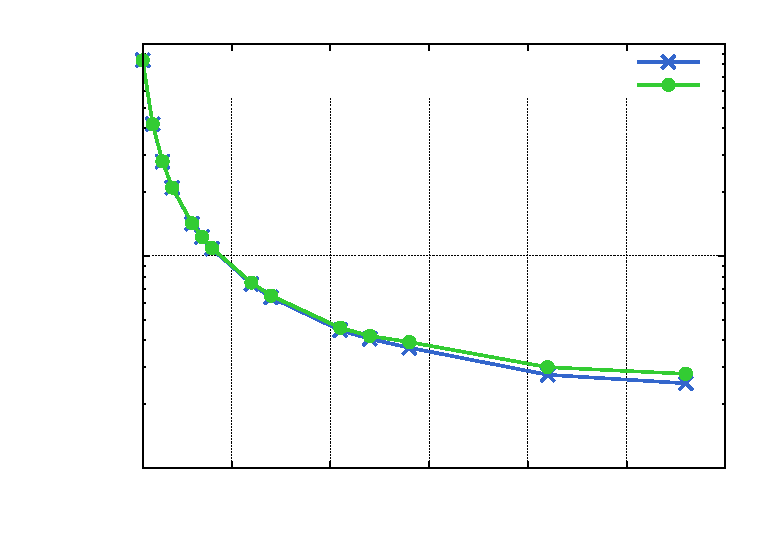
\includegraphics{plot-T-UDN-SM_nogatherInt_selected_500_selected_168_slide_2}}%
    \gplfronttext
  \end{picture}%
\endgroup
}      
    \end{tabular}
  \end{center}
  \begin{columns}[b]
    \column{1.15in}
    \begin{tabular}{c}
      \tiny Dimensione delle matrici 280x280 \\
      \resizebox{!}{1.15in}{% GNUPLOT: LaTeX picture with Postscript
\begingroup
  \makeatletter
  \providecommand\color[2][]{%
    \GenericError{(gnuplot) \space\space\space\@spaces}{%
      Package color not loaded in conjunction with
      terminal option `colourtext'%
    }{See the gnuplot documentation for explanation.%
    }{Either use 'blacktext' in gnuplot or load the package
      color.sty in LaTeX.}%
    \renewcommand\color[2][]{}%
  }%
  \providecommand\includegraphics[2][]{%
    \GenericError{(gnuplot) \space\space\space\@spaces}{%
      Package graphicx or graphics not loaded%
    }{See the gnuplot documentation for explanation.%
    }{The gnuplot epslatex terminal needs graphicx.sty or graphics.sty.}%
    \renewcommand\includegraphics[2][]{}%
  }%
  \providecommand\rotatebox[2]{#2}%
  \@ifundefined{ifGPcolor}{%
    \newif\ifGPcolor
    \GPcolortrue
  }{}%
  \@ifundefined{ifGPblacktext}{%
    \newif\ifGPblacktext
    \GPblacktexttrue
  }{}%
  % define a \g@addto@macro without @ in the name:
  \let\gplgaddtomacro\g@addto@macro
  % define empty templates for all commands taking text:
  \gdef\gplbacktext{}%
  \gdef\gplfronttext{}%
  \makeatother
  \ifGPblacktext
    % no textcolor at all
    \def\colorrgb#1{}%
    \def\colorgray#1{}%
  \else
    % gray or color?
    \ifGPcolor
      \def\colorrgb#1{\color[rgb]{#1}}%
      \def\colorgray#1{\color[gray]{#1}}%
      \expandafter\def\csname LTw\endcsname{\color{white}}%
      \expandafter\def\csname LTb\endcsname{\color{black}}%
      \expandafter\def\csname LTa\endcsname{\color{black}}%
      \expandafter\def\csname LT0\endcsname{\color[rgb]{1,0,0}}%
      \expandafter\def\csname LT1\endcsname{\color[rgb]{0,1,0}}%
      \expandafter\def\csname LT2\endcsname{\color[rgb]{0,0,1}}%
      \expandafter\def\csname LT3\endcsname{\color[rgb]{1,0,1}}%
      \expandafter\def\csname LT4\endcsname{\color[rgb]{0,1,1}}%
      \expandafter\def\csname LT5\endcsname{\color[rgb]{1,1,0}}%
      \expandafter\def\csname LT6\endcsname{\color[rgb]{0,0,0}}%
      \expandafter\def\csname LT7\endcsname{\color[rgb]{1,0.3,0}}%
      \expandafter\def\csname LT8\endcsname{\color[rgb]{0.5,0.5,0.5}}%
    \else
      % gray
      \def\colorrgb#1{\color{black}}%
      \def\colorgray#1{\color[gray]{#1}}%
      \expandafter\def\csname LTw\endcsname{\color{white}}%
      \expandafter\def\csname LTb\endcsname{\color{black}}%
      \expandafter\def\csname LTa\endcsname{\color{black}}%
      \expandafter\def\csname LT0\endcsname{\color{black}}%
      \expandafter\def\csname LT1\endcsname{\color{black}}%
      \expandafter\def\csname LT2\endcsname{\color{black}}%
      \expandafter\def\csname LT3\endcsname{\color{black}}%
      \expandafter\def\csname LT4\endcsname{\color{black}}%
      \expandafter\def\csname LT5\endcsname{\color{black}}%
      \expandafter\def\csname LT6\endcsname{\color{black}}%
      \expandafter\def\csname LT7\endcsname{\color{black}}%
      \expandafter\def\csname LT8\endcsname{\color{black}}%
    \fi
  \fi
  \setlength{\unitlength}{0.0500bp}%
  \begin{picture}(7200.00,5040.00)%
    \gplgaddtomacro\gplbacktext{%
      \csname LTb\endcsname%
      \put(1210,704){\makebox(0,0)[r]{\strut{} 10}}%
      \csname LTb\endcsname%
      \put(1210,2061){\makebox(0,0)[r]{\strut{} 100}}%
      \csname LTb\endcsname%
      \put(1210,3418){\makebox(0,0)[r]{\strut{} 1000}}%
      \csname LTb\endcsname%
      \put(1210,4775){\makebox(0,0)[r]{\strut{} 10000}}%
      \csname LTb\endcsname%
      \put(2175,484){\makebox(0,0){\strut{} 10}}%
      \csname LTb\endcsname%
      \put(3101,484){\makebox(0,0){\strut{} 20}}%
      \csname LTb\endcsname%
      \put(4026,484){\makebox(0,0){\strut{} 30}}%
      \csname LTb\endcsname%
      \put(4952,484){\makebox(0,0){\strut{} 40}}%
      \csname LTb\endcsname%
      \put(5877,484){\makebox(0,0){\strut{} 50}}%
      \csname LTb\endcsname%
      \put(6803,484){\makebox(0,0){\strut{} 60}}%
      \put(176,2739){\rotatebox{-270}{\makebox(0,0){\strut{}service time ($\,\mu\mathrm{sec}$\,)}}}%
      \put(4072,154){\makebox(0,0){\strut{}$n$ parallel degree}}%
    }%
    \gplgaddtomacro\gplfronttext{%
      \csname LTb\endcsname%
      \put(5962,4602){\makebox(0,0)[r]{\strut{}uso della Rete di Interconnessione}}%
      \csname LTb\endcsname%
      \put(5962,4382){\makebox(0,0)[r]{\strut{}uso della Memoria Condivisa}}%
    }%
    \gplbacktext
    \put(0,0){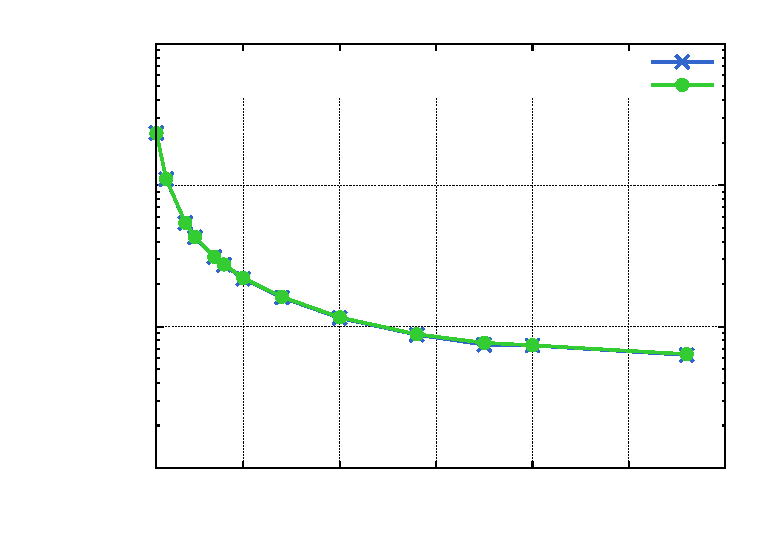
\includegraphics{plot-T-UDN-SM_nogatherInt_selected_500_selected_280_slide_2}}%
    \gplfronttext
  \end{picture}%
\endgroup
}       
    \end{tabular}
    \column{.45\textwidth}
    \hspace{5mm}
    \begin{center}
    \tiny \emph{Differenza tra i migliori tempi di servizio}

    \vspace{2mm}

    \begin{tabular}{cr}
      \tiny 56x56 & \scriptsize 2.558  \musec \\ %2211.562
      \tiny 168x168 & \scriptsize  2.718 \musec \\ %2349.687
      \tiny 280x280 & \scriptsize  0.951 \musec \\ %821.906
    \end{tabular}
    \end{center}
  \end{columns}
\end{frame}


\begin{frame}
  \frametitle{Confronto: tempo di servizio Multicast}
  \framesubtitle{Misurazione con il sottosistema parallelo non collo di bottiglia}
  \begin{itemize}
  \item \small il tempo di servizio della multicast implementata con un albero binario \`e in media la latenza di due comunicazioni sul canale simmetrico
  \end{itemize}
  \begin{center}
    \begin{tabular}{cc}
      \tiny Dimensione delle matrici 56x56 &
      \tiny Dimensione delle matrici 280x280 \\
      \resizebox{.5\columnwidth}{!}{% GNUPLOT: LaTeX picture with Postscript
\begingroup
  \makeatletter
  \providecommand\color[2][]{%
    \GenericError{(gnuplot) \space\space\space\@spaces}{%
      Package color not loaded in conjunction with
      terminal option `colourtext'%
    }{See the gnuplot documentation for explanation.%
    }{Either use 'blacktext' in gnuplot or load the package
      color.sty in LaTeX.}%
    \renewcommand\color[2][]{}%
  }%
  \providecommand\includegraphics[2][]{%
    \GenericError{(gnuplot) \space\space\space\@spaces}{%
      Package graphicx or graphics not loaded%
    }{See the gnuplot documentation for explanation.%
    }{The gnuplot epslatex terminal needs graphicx.sty or graphics.sty.}%
    \renewcommand\includegraphics[2][]{}%
  }%
  \providecommand\rotatebox[2]{#2}%
  \@ifundefined{ifGPcolor}{%
    \newif\ifGPcolor
    \GPcolortrue
  }{}%
  \@ifundefined{ifGPblacktext}{%
    \newif\ifGPblacktext
    \GPblacktexttrue
  }{}%
  % define a \g@addto@macro without @ in the name:
  \let\gplgaddtomacro\g@addto@macro
  % define empty templates for all commands taking text:
  \gdef\gplbacktext{}%
  \gdef\gplfronttext{}%
  \makeatother
  \ifGPblacktext
    % no textcolor at all
    \def\colorrgb#1{}%
    \def\colorgray#1{}%
  \else
    % gray or color?
    \ifGPcolor
      \def\colorrgb#1{\color[rgb]{#1}}%
      \def\colorgray#1{\color[gray]{#1}}%
      \expandafter\def\csname LTw\endcsname{\color{white}}%
      \expandafter\def\csname LTb\endcsname{\color{black}}%
      \expandafter\def\csname LTa\endcsname{\color{black}}%
      \expandafter\def\csname LT0\endcsname{\color[rgb]{1,0,0}}%
      \expandafter\def\csname LT1\endcsname{\color[rgb]{0,1,0}}%
      \expandafter\def\csname LT2\endcsname{\color[rgb]{0,0,1}}%
      \expandafter\def\csname LT3\endcsname{\color[rgb]{1,0,1}}%
      \expandafter\def\csname LT4\endcsname{\color[rgb]{0,1,1}}%
      \expandafter\def\csname LT5\endcsname{\color[rgb]{1,1,0}}%
      \expandafter\def\csname LT6\endcsname{\color[rgb]{0,0,0}}%
      \expandafter\def\csname LT7\endcsname{\color[rgb]{1,0.3,0}}%
      \expandafter\def\csname LT8\endcsname{\color[rgb]{0.5,0.5,0.5}}%
    \else
      % gray
      \def\colorrgb#1{\color{black}}%
      \def\colorgray#1{\color[gray]{#1}}%
      \expandafter\def\csname LTw\endcsname{\color{white}}%
      \expandafter\def\csname LTb\endcsname{\color{black}}%
      \expandafter\def\csname LTa\endcsname{\color{black}}%
      \expandafter\def\csname LT0\endcsname{\color{black}}%
      \expandafter\def\csname LT1\endcsname{\color{black}}%
      \expandafter\def\csname LT2\endcsname{\color{black}}%
      \expandafter\def\csname LT3\endcsname{\color{black}}%
      \expandafter\def\csname LT4\endcsname{\color{black}}%
      \expandafter\def\csname LT5\endcsname{\color{black}}%
      \expandafter\def\csname LT6\endcsname{\color{black}}%
      \expandafter\def\csname LT7\endcsname{\color{black}}%
      \expandafter\def\csname LT8\endcsname{\color{black}}%
    \fi
  \fi
  \setlength{\unitlength}{0.0500bp}%
  \begin{picture}(7200.00,5040.00)%
    \gplgaddtomacro\gplbacktext{%
      \csname LTb\endcsname%
      \put(946,704){\makebox(0,0)[r]{\strut{} 0}}%
      \csname LTb\endcsname%
      \put(946,1629){\makebox(0,0)[r]{\strut{} 0.5}}%
      \csname LTb\endcsname%
      \put(946,2554){\makebox(0,0)[r]{\strut{} 1}}%
      \csname LTb\endcsname%
      \put(946,3480){\makebox(0,0)[r]{\strut{} 1.5}}%
      \csname LTb\endcsname%
      \put(946,4405){\makebox(0,0)[r]{\strut{} 2}}%
      \csname LTb\endcsname%
      \put(1951,484){\makebox(0,0){\strut{} 10}}%
      \csname LTb\endcsname%
      \put(2922,484){\makebox(0,0){\strut{} 20}}%
      \csname LTb\endcsname%
      \put(3892,484){\makebox(0,0){\strut{} 30}}%
      \csname LTb\endcsname%
      \put(4862,484){\makebox(0,0){\strut{} 40}}%
      \csname LTb\endcsname%
      \put(5833,484){\makebox(0,0){\strut{} 50}}%
      \csname LTb\endcsname%
      \put(6803,484){\makebox(0,0){\strut{} 60}}%
      \put(176,2739){\rotatebox{-270}{\makebox(0,0){\strut{}multicast service time $(\,\mu\textrm{sec}\,)$}}}%
      \put(3940,154){\makebox(0,0){\strut{}$n$ parallel degree}}%
    }%
    \gplgaddtomacro\gplfronttext{%
      \csname LTb\endcsname%
      \put(2134,4602){\makebox(0,0)[r]{\strut{}udn udn}}%
      \csname LTb\endcsname%
      \put(2134,4382){\makebox(0,0)[r]{\strut{}sm sm}}%
    }%
    \gplbacktext
    \put(0,0){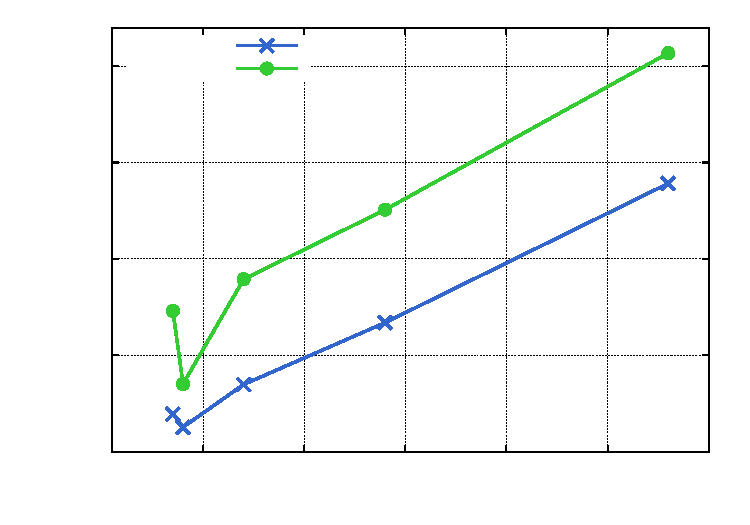
\includegraphics{plot-Tmult-UDN-SM-millis_nogatherInt_selected_500_selected_56_slide}}%
    \gplfronttext
  \end{picture}%
\endgroup
} &
      \resizebox{.5\columnwidth}{!}{% GNUPLOT: LaTeX picture with Postscript
\begingroup
  \makeatletter
  \providecommand\color[2][]{%
    \GenericError{(gnuplot) \space\space\space\@spaces}{%
      Package color not loaded in conjunction with
      terminal option `colourtext'%
    }{See the gnuplot documentation for explanation.%
    }{Either use 'blacktext' in gnuplot or load the package
      color.sty in LaTeX.}%
    \renewcommand\color[2][]{}%
  }%
  \providecommand\includegraphics[2][]{%
    \GenericError{(gnuplot) \space\space\space\@spaces}{%
      Package graphicx or graphics not loaded%
    }{See the gnuplot documentation for explanation.%
    }{The gnuplot epslatex terminal needs graphicx.sty or graphics.sty.}%
    \renewcommand\includegraphics[2][]{}%
  }%
  \providecommand\rotatebox[2]{#2}%
  \@ifundefined{ifGPcolor}{%
    \newif\ifGPcolor
    \GPcolortrue
  }{}%
  \@ifundefined{ifGPblacktext}{%
    \newif\ifGPblacktext
    \GPblacktexttrue
  }{}%
  % define a \g@addto@macro without @ in the name:
  \let\gplgaddtomacro\g@addto@macro
  % define empty templates for all commands taking text:
  \gdef\gplbacktext{}%
  \gdef\gplfronttext{}%
  \makeatother
  \ifGPblacktext
    % no textcolor at all
    \def\colorrgb#1{}%
    \def\colorgray#1{}%
  \else
    % gray or color?
    \ifGPcolor
      \def\colorrgb#1{\color[rgb]{#1}}%
      \def\colorgray#1{\color[gray]{#1}}%
      \expandafter\def\csname LTw\endcsname{\color{white}}%
      \expandafter\def\csname LTb\endcsname{\color{black}}%
      \expandafter\def\csname LTa\endcsname{\color{black}}%
      \expandafter\def\csname LT0\endcsname{\color[rgb]{1,0,0}}%
      \expandafter\def\csname LT1\endcsname{\color[rgb]{0,1,0}}%
      \expandafter\def\csname LT2\endcsname{\color[rgb]{0,0,1}}%
      \expandafter\def\csname LT3\endcsname{\color[rgb]{1,0,1}}%
      \expandafter\def\csname LT4\endcsname{\color[rgb]{0,1,1}}%
      \expandafter\def\csname LT5\endcsname{\color[rgb]{1,1,0}}%
      \expandafter\def\csname LT6\endcsname{\color[rgb]{0,0,0}}%
      \expandafter\def\csname LT7\endcsname{\color[rgb]{1,0.3,0}}%
      \expandafter\def\csname LT8\endcsname{\color[rgb]{0.5,0.5,0.5}}%
    \else
      % gray
      \def\colorrgb#1{\color{black}}%
      \def\colorgray#1{\color[gray]{#1}}%
      \expandafter\def\csname LTw\endcsname{\color{white}}%
      \expandafter\def\csname LTb\endcsname{\color{black}}%
      \expandafter\def\csname LTa\endcsname{\color{black}}%
      \expandafter\def\csname LT0\endcsname{\color{black}}%
      \expandafter\def\csname LT1\endcsname{\color{black}}%
      \expandafter\def\csname LT2\endcsname{\color{black}}%
      \expandafter\def\csname LT3\endcsname{\color{black}}%
      \expandafter\def\csname LT4\endcsname{\color{black}}%
      \expandafter\def\csname LT5\endcsname{\color{black}}%
      \expandafter\def\csname LT6\endcsname{\color{black}}%
      \expandafter\def\csname LT7\endcsname{\color{black}}%
      \expandafter\def\csname LT8\endcsname{\color{black}}%
    \fi
  \fi
  \setlength{\unitlength}{0.0500bp}%
  \begin{picture}(7200.00,5040.00)%
    \gplgaddtomacro\gplbacktext{%
      \csname LTb\endcsname%
      \put(946,704){\makebox(0,0)[r]{\strut{} 0}}%
      \csname LTb\endcsname%
      \put(946,1629){\makebox(0,0)[r]{\strut{} 0.5}}%
      \csname LTb\endcsname%
      \put(946,2554){\makebox(0,0)[r]{\strut{} 1}}%
      \csname LTb\endcsname%
      \put(946,3480){\makebox(0,0)[r]{\strut{} 1.5}}%
      \csname LTb\endcsname%
      \put(946,4405){\makebox(0,0)[r]{\strut{} 2}}%
      \csname LTb\endcsname%
      \put(1951,484){\makebox(0,0){\strut{} 10}}%
      \csname LTb\endcsname%
      \put(2922,484){\makebox(0,0){\strut{} 20}}%
      \csname LTb\endcsname%
      \put(3892,484){\makebox(0,0){\strut{} 30}}%
      \csname LTb\endcsname%
      \put(4862,484){\makebox(0,0){\strut{} 40}}%
      \csname LTb\endcsname%
      \put(5833,484){\makebox(0,0){\strut{} 50}}%
      \csname LTb\endcsname%
      \put(6803,484){\makebox(0,0){\strut{} 60}}%
      \put(176,2739){\rotatebox{-270}{\makebox(0,0){\strut{}multicast service time $(\,\mu\textrm{sec}\,)$}}}%
      \put(3940,154){\makebox(0,0){\strut{}$n$ parallel degree}}%
    }%
    \gplgaddtomacro\gplfronttext{%
      \csname LTb\endcsname%
      \put(2134,4602){\makebox(0,0)[r]{\strut{}udn udn}}%
      \csname LTb\endcsname%
      \put(2134,4382){\makebox(0,0)[r]{\strut{}sm sm}}%
    }%
    \gplbacktext
    \put(0,0){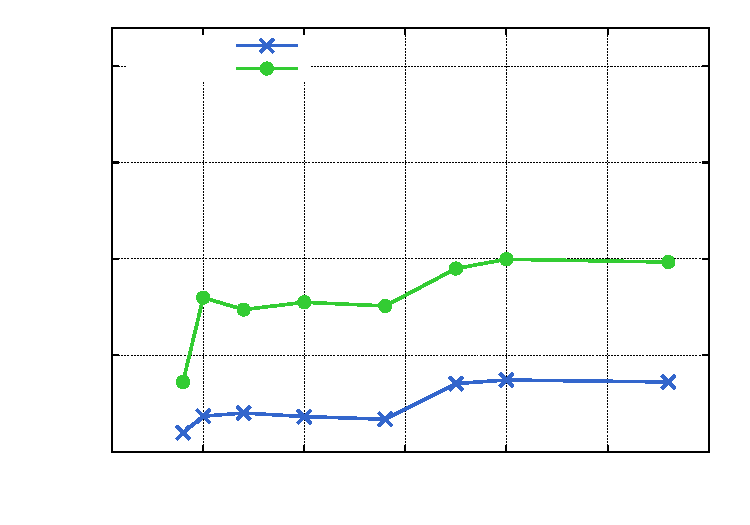
\includegraphics{plot-Tmult-UDN-SM-millis_nogatherInt_selected_500_selected_280_slide}}%
    \gplfronttext
  \end{picture}%
\endgroup
}
    \end{tabular}
  \end{center}
\end{frame}

%% \begin{frame}
%%   \frametitle{Confronto: Tempo di calcolo di un singolo prodotto scalare}
%%   \framesubtitle{Misurazione con il sottosistema parallelo collo di bottiglia}
%%   \begin{center}
%%     \begin{tabular}{cc}
%%       \tiny Dimensione delle matrici 56x56 &
%%       \tiny Dimensione delle matrici 168x168 \\
%%       \resizebox{.5\columnwidth}{!}{% GNUPLOT: LaTeX picture with Postscript
\begingroup
  \makeatletter
  \providecommand\color[2][]{%
    \GenericError{(gnuplot) \space\space\space\@spaces}{%
      Package color not loaded in conjunction with
      terminal option `colourtext'%
    }{See the gnuplot documentation for explanation.%
    }{Either use 'blacktext' in gnuplot or load the package
      color.sty in LaTeX.}%
    \renewcommand\color[2][]{}%
  }%
  \providecommand\includegraphics[2][]{%
    \GenericError{(gnuplot) \space\space\space\@spaces}{%
      Package graphicx or graphics not loaded%
    }{See the gnuplot documentation for explanation.%
    }{The gnuplot epslatex terminal needs graphicx.sty or graphics.sty.}%
    \renewcommand\includegraphics[2][]{}%
  }%
  \providecommand\rotatebox[2]{#2}%
  \@ifundefined{ifGPcolor}{%
    \newif\ifGPcolor
    \GPcolortrue
  }{}%
  \@ifundefined{ifGPblacktext}{%
    \newif\ifGPblacktext
    \GPblacktextfalse
  }{}%
  % define a \g@addto@macro without @ in the name:
  \let\gplgaddtomacro\g@addto@macro
  % define empty templates for all commands taking text:
  \gdef\gplbacktext{}%
  \gdef\gplfronttext{}%
  \makeatother
  \ifGPblacktext
    % no textcolor at all
    \def\colorrgb#1{}%
    \def\colorgray#1{}%
  \else
    % gray or color?
    \ifGPcolor
      \def\colorrgb#1{\color[rgb]{#1}}%
      \def\colorgray#1{\color[gray]{#1}}%
      \expandafter\def\csname LTw\endcsname{\color{white}}%
      \expandafter\def\csname LTb\endcsname{\color{black}}%
      \expandafter\def\csname LTa\endcsname{\color{black}}%
      \expandafter\def\csname LT0\endcsname{\color[rgb]{1,0,0}}%
      \expandafter\def\csname LT1\endcsname{\color[rgb]{0,1,0}}%
      \expandafter\def\csname LT2\endcsname{\color[rgb]{0,0,1}}%
      \expandafter\def\csname LT3\endcsname{\color[rgb]{1,0,1}}%
      \expandafter\def\csname LT4\endcsname{\color[rgb]{0,1,1}}%
      \expandafter\def\csname LT5\endcsname{\color[rgb]{1,1,0}}%
      \expandafter\def\csname LT6\endcsname{\color[rgb]{0,0,0}}%
      \expandafter\def\csname LT7\endcsname{\color[rgb]{1,0.3,0}}%
      \expandafter\def\csname LT8\endcsname{\color[rgb]{0.5,0.5,0.5}}%
    \else
      % gray
      \def\colorrgb#1{\color{black}}%
      \def\colorgray#1{\color[gray]{#1}}%
      \expandafter\def\csname LTw\endcsname{\color{white}}%
      \expandafter\def\csname LTb\endcsname{\color{black}}%
      \expandafter\def\csname LTa\endcsname{\color{black}}%
      \expandafter\def\csname LT0\endcsname{\color{black}}%
      \expandafter\def\csname LT1\endcsname{\color{black}}%
      \expandafter\def\csname LT2\endcsname{\color{black}}%
      \expandafter\def\csname LT3\endcsname{\color{black}}%
      \expandafter\def\csname LT4\endcsname{\color{black}}%
      \expandafter\def\csname LT5\endcsname{\color{black}}%
      \expandafter\def\csname LT6\endcsname{\color{black}}%
      \expandafter\def\csname LT7\endcsname{\color{black}}%
      \expandafter\def\csname LT8\endcsname{\color{black}}%
    \fi
  \fi
  \setlength{\unitlength}{0.0500bp}%
  \begin{picture}(7200.00,5040.00)%
    \gplgaddtomacro\gplbacktext{%
      \csname LTb\endcsname%
      \put(946,1074){\makebox(0,0)[r]{\strut{} 1}}%
      \csname LTb\endcsname%
      \put(946,1999){\makebox(0,0)[r]{\strut{} 1.5}}%
      \csname LTb\endcsname%
      \put(946,2925){\makebox(0,0)[r]{\strut{} 2}}%
      \csname LTb\endcsname%
      \put(946,3850){\makebox(0,0)[r]{\strut{} 2.5}}%
      \csname LTb\endcsname%
      \put(946,4775){\makebox(0,0)[r]{\strut{} 3}}%
      \csname LTb\endcsname%
      \put(1951,484){\makebox(0,0){\strut{} 10}}%
      \csname LTb\endcsname%
      \put(2922,484){\makebox(0,0){\strut{} 20}}%
      \csname LTb\endcsname%
      \put(3892,484){\makebox(0,0){\strut{} 30}}%
      \csname LTb\endcsname%
      \put(4862,484){\makebox(0,0){\strut{} 40}}%
      \csname LTb\endcsname%
      \put(5833,484){\makebox(0,0){\strut{} 50}}%
      \csname LTb\endcsname%
      \put(6803,484){\makebox(0,0){\strut{} 60}}%
      \put(176,2739){\rotatebox{-270}{\makebox(0,0){\strut{}$T_{\textrm{row}}^{\phantom{row}(n)} / T_{\textrm{row}}^{\phantom{row}(1)}$}}}%
      \put(3940,154){\makebox(0,0){\strut{}$n$ parallel degree}}%
    }%
    \gplgaddtomacro\gplfronttext{%
      \csname LTb\endcsname%
      \put(5698,4602){\makebox(0,0)[r]{\strut{}uso della Rete di Interconnessione}}%
      \csname LTb\endcsname%
      \put(5698,4382){\makebox(0,0)[r]{\strut{}uso della Memoria Condivisa}}%
    }%
    \gplbacktext
    \put(0,0){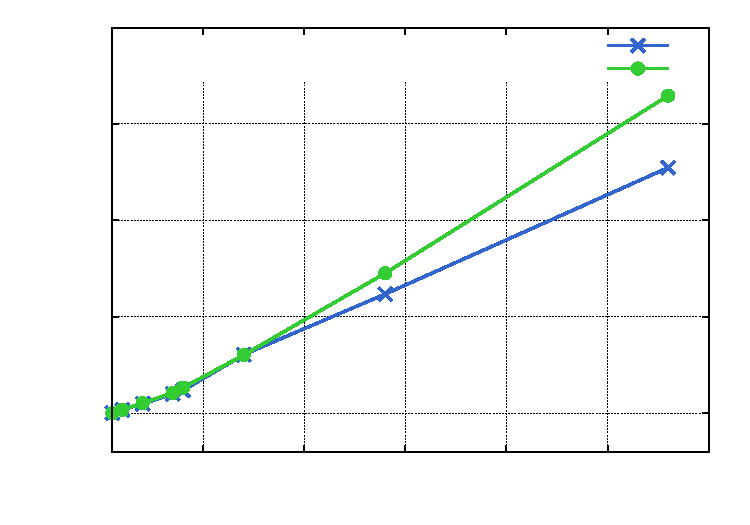
\includegraphics{plot-comp-rowCalcT_nogatherInt_all_500_4000_56_slide_2}}%
    \gplfronttext
  \end{picture}%
\endgroup
} &
%%       \resizebox{.5\columnwidth}{!}{% GNUPLOT: LaTeX picture with Postscript
\begingroup
  \makeatletter
  \providecommand\color[2][]{%
    \GenericError{(gnuplot) \space\space\space\@spaces}{%
      Package color not loaded in conjunction with
      terminal option `colourtext'%
    }{See the gnuplot documentation for explanation.%
    }{Either use 'blacktext' in gnuplot or load the package
      color.sty in LaTeX.}%
    \renewcommand\color[2][]{}%
  }%
  \providecommand\includegraphics[2][]{%
    \GenericError{(gnuplot) \space\space\space\@spaces}{%
      Package graphicx or graphics not loaded%
    }{See the gnuplot documentation for explanation.%
    }{The gnuplot epslatex terminal needs graphicx.sty or graphics.sty.}%
    \renewcommand\includegraphics[2][]{}%
  }%
  \providecommand\rotatebox[2]{#2}%
  \@ifundefined{ifGPcolor}{%
    \newif\ifGPcolor
    \GPcolortrue
  }{}%
  \@ifundefined{ifGPblacktext}{%
    \newif\ifGPblacktext
    \GPblacktextfalse
  }{}%
  % define a \g@addto@macro without @ in the name:
  \let\gplgaddtomacro\g@addto@macro
  % define empty templates for all commands taking text:
  \gdef\gplbacktext{}%
  \gdef\gplfronttext{}%
  \makeatother
  \ifGPblacktext
    % no textcolor at all
    \def\colorrgb#1{}%
    \def\colorgray#1{}%
  \else
    % gray or color?
    \ifGPcolor
      \def\colorrgb#1{\color[rgb]{#1}}%
      \def\colorgray#1{\color[gray]{#1}}%
      \expandafter\def\csname LTw\endcsname{\color{white}}%
      \expandafter\def\csname LTb\endcsname{\color{black}}%
      \expandafter\def\csname LTa\endcsname{\color{black}}%
      \expandafter\def\csname LT0\endcsname{\color[rgb]{1,0,0}}%
      \expandafter\def\csname LT1\endcsname{\color[rgb]{0,1,0}}%
      \expandafter\def\csname LT2\endcsname{\color[rgb]{0,0,1}}%
      \expandafter\def\csname LT3\endcsname{\color[rgb]{1,0,1}}%
      \expandafter\def\csname LT4\endcsname{\color[rgb]{0,1,1}}%
      \expandafter\def\csname LT5\endcsname{\color[rgb]{1,1,0}}%
      \expandafter\def\csname LT6\endcsname{\color[rgb]{0,0,0}}%
      \expandafter\def\csname LT7\endcsname{\color[rgb]{1,0.3,0}}%
      \expandafter\def\csname LT8\endcsname{\color[rgb]{0.5,0.5,0.5}}%
    \else
      % gray
      \def\colorrgb#1{\color{black}}%
      \def\colorgray#1{\color[gray]{#1}}%
      \expandafter\def\csname LTw\endcsname{\color{white}}%
      \expandafter\def\csname LTb\endcsname{\color{black}}%
      \expandafter\def\csname LTa\endcsname{\color{black}}%
      \expandafter\def\csname LT0\endcsname{\color{black}}%
      \expandafter\def\csname LT1\endcsname{\color{black}}%
      \expandafter\def\csname LT2\endcsname{\color{black}}%
      \expandafter\def\csname LT3\endcsname{\color{black}}%
      \expandafter\def\csname LT4\endcsname{\color{black}}%
      \expandafter\def\csname LT5\endcsname{\color{black}}%
      \expandafter\def\csname LT6\endcsname{\color{black}}%
      \expandafter\def\csname LT7\endcsname{\color{black}}%
      \expandafter\def\csname LT8\endcsname{\color{black}}%
    \fi
  \fi
  \setlength{\unitlength}{0.0500bp}%
  \begin{picture}(7200.00,5040.00)%
    \gplgaddtomacro\gplbacktext{%
      \csname LTb\endcsname%
      \put(946,1074){\makebox(0,0)[r]{\strut{} 1}}%
      \csname LTb\endcsname%
      \put(946,1999){\makebox(0,0)[r]{\strut{} 1.5}}%
      \csname LTb\endcsname%
      \put(946,2925){\makebox(0,0)[r]{\strut{} 2}}%
      \csname LTb\endcsname%
      \put(946,3850){\makebox(0,0)[r]{\strut{} 2.5}}%
      \csname LTb\endcsname%
      \put(946,4775){\makebox(0,0)[r]{\strut{} 3}}%
      \csname LTb\endcsname%
      \put(1951,484){\makebox(0,0){\strut{} 10}}%
      \csname LTb\endcsname%
      \put(2922,484){\makebox(0,0){\strut{} 20}}%
      \csname LTb\endcsname%
      \put(3892,484){\makebox(0,0){\strut{} 30}}%
      \csname LTb\endcsname%
      \put(4862,484){\makebox(0,0){\strut{} 40}}%
      \csname LTb\endcsname%
      \put(5833,484){\makebox(0,0){\strut{} 50}}%
      \csname LTb\endcsname%
      \put(6803,484){\makebox(0,0){\strut{} 60}}%
      \put(176,2739){\rotatebox{-270}{\makebox(0,0){\strut{}$T_{\textrm{row}}^{\phantom{row}(n)} / T_{\textrm{row}}^{\phantom{row}(1)}$}}}%
      \put(3940,154){\makebox(0,0){\strut{}$n$ parallel degree}}%
    }%
    \gplgaddtomacro\gplfronttext{%
      \csname LTb\endcsname%
      \put(5698,4602){\makebox(0,0)[r]{\strut{}uso della Rete di Interconnessione}}%
      \csname LTb\endcsname%
      \put(5698,4382){\makebox(0,0)[r]{\strut{}uso della Memoria Condivisa}}%
    }%
    \gplbacktext
    \put(0,0){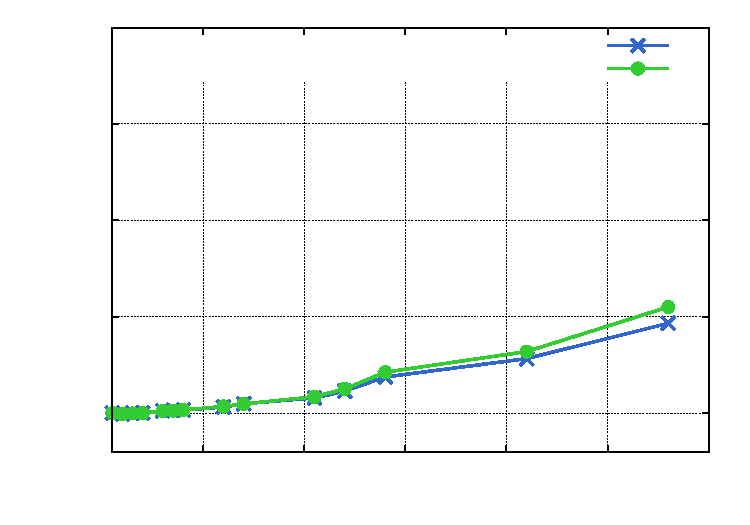
\includegraphics{plot-comp-rowCalcT_nogatherInt_all_500_4000_168_slide_2}}%
    \gplfronttext
  \end{picture}%
\endgroup
} \\
%%     \end{tabular}
%%   \end{center}
%% \end{frame}


%% \begin{frame}
%%   \frametitle{Confronto: Tempo di calcolo di un singolo prodotto scalare}
%%   \framesubtitle{Dimensione della matrice 56x56}
%%   \begin{columns}[c]
%%   \column{.5\textwidth}
%%   {\small Matrice di Interi}
%%   \column{.5\textwidth}
%%   {\small Matrice di Float}
%% \end{columns}
%% \vspace{5mm}
%% \begin{columns}[c]
%%     \column{.5\textwidth}
%%     \resizebox{\columnwidth}{!}{% GNUPLOT: LaTeX picture with Postscript
\begingroup
  \makeatletter
  \providecommand\color[2][]{%
    \GenericError{(gnuplot) \space\space\space\@spaces}{%
      Package color not loaded in conjunction with
      terminal option `colourtext'%
    }{See the gnuplot documentation for explanation.%
    }{Either use 'blacktext' in gnuplot or load the package
      color.sty in LaTeX.}%
    \renewcommand\color[2][]{}%
  }%
  \providecommand\includegraphics[2][]{%
    \GenericError{(gnuplot) \space\space\space\@spaces}{%
      Package graphicx or graphics not loaded%
    }{See the gnuplot documentation for explanation.%
    }{The gnuplot epslatex terminal needs graphicx.sty or graphics.sty.}%
    \renewcommand\includegraphics[2][]{}%
  }%
  \providecommand\rotatebox[2]{#2}%
  \@ifundefined{ifGPcolor}{%
    \newif\ifGPcolor
    \GPcolortrue
  }{}%
  \@ifundefined{ifGPblacktext}{%
    \newif\ifGPblacktext
    \GPblacktextfalse
  }{}%
  % define a \g@addto@macro without @ in the name:
  \let\gplgaddtomacro\g@addto@macro
  % define empty templates for all commands taking text:
  \gdef\gplbacktext{}%
  \gdef\gplfronttext{}%
  \makeatother
  \ifGPblacktext
    % no textcolor at all
    \def\colorrgb#1{}%
    \def\colorgray#1{}%
  \else
    % gray or color?
    \ifGPcolor
      \def\colorrgb#1{\color[rgb]{#1}}%
      \def\colorgray#1{\color[gray]{#1}}%
      \expandafter\def\csname LTw\endcsname{\color{white}}%
      \expandafter\def\csname LTb\endcsname{\color{black}}%
      \expandafter\def\csname LTa\endcsname{\color{black}}%
      \expandafter\def\csname LT0\endcsname{\color[rgb]{1,0,0}}%
      \expandafter\def\csname LT1\endcsname{\color[rgb]{0,1,0}}%
      \expandafter\def\csname LT2\endcsname{\color[rgb]{0,0,1}}%
      \expandafter\def\csname LT3\endcsname{\color[rgb]{1,0,1}}%
      \expandafter\def\csname LT4\endcsname{\color[rgb]{0,1,1}}%
      \expandafter\def\csname LT5\endcsname{\color[rgb]{1,1,0}}%
      \expandafter\def\csname LT6\endcsname{\color[rgb]{0,0,0}}%
      \expandafter\def\csname LT7\endcsname{\color[rgb]{1,0.3,0}}%
      \expandafter\def\csname LT8\endcsname{\color[rgb]{0.5,0.5,0.5}}%
    \else
      % gray
      \def\colorrgb#1{\color{black}}%
      \def\colorgray#1{\color[gray]{#1}}%
      \expandafter\def\csname LTw\endcsname{\color{white}}%
      \expandafter\def\csname LTb\endcsname{\color{black}}%
      \expandafter\def\csname LTa\endcsname{\color{black}}%
      \expandafter\def\csname LT0\endcsname{\color{black}}%
      \expandafter\def\csname LT1\endcsname{\color{black}}%
      \expandafter\def\csname LT2\endcsname{\color{black}}%
      \expandafter\def\csname LT3\endcsname{\color{black}}%
      \expandafter\def\csname LT4\endcsname{\color{black}}%
      \expandafter\def\csname LT5\endcsname{\color{black}}%
      \expandafter\def\csname LT6\endcsname{\color{black}}%
      \expandafter\def\csname LT7\endcsname{\color{black}}%
      \expandafter\def\csname LT8\endcsname{\color{black}}%
    \fi
  \fi
  \setlength{\unitlength}{0.0500bp}%
  \begin{picture}(7200.00,5040.00)%
    \gplgaddtomacro\gplbacktext{%
      \csname LTb\endcsname%
      \put(946,1074){\makebox(0,0)[r]{\strut{} 1}}%
      \csname LTb\endcsname%
      \put(946,1999){\makebox(0,0)[r]{\strut{} 1.5}}%
      \csname LTb\endcsname%
      \put(946,2925){\makebox(0,0)[r]{\strut{} 2}}%
      \csname LTb\endcsname%
      \put(946,3850){\makebox(0,0)[r]{\strut{} 2.5}}%
      \csname LTb\endcsname%
      \put(946,4775){\makebox(0,0)[r]{\strut{} 3}}%
      \csname LTb\endcsname%
      \put(1951,484){\makebox(0,0){\strut{} 10}}%
      \csname LTb\endcsname%
      \put(2922,484){\makebox(0,0){\strut{} 20}}%
      \csname LTb\endcsname%
      \put(3892,484){\makebox(0,0){\strut{} 30}}%
      \csname LTb\endcsname%
      \put(4862,484){\makebox(0,0){\strut{} 40}}%
      \csname LTb\endcsname%
      \put(5833,484){\makebox(0,0){\strut{} 50}}%
      \csname LTb\endcsname%
      \put(6803,484){\makebox(0,0){\strut{} 60}}%
      \put(176,2739){\rotatebox{-270}{\makebox(0,0){\strut{}$T_{\textrm{row}}^{\phantom{row}(n)} / T_{\textrm{row}}^{\phantom{row}(1)}$}}}%
      \put(3940,154){\makebox(0,0){\strut{}$n$ parallel degree}}%
    }%
    \gplgaddtomacro\gplfronttext{%
      \csname LTb\endcsname%
      \put(5698,4602){\makebox(0,0)[r]{\strut{}uso della Rete di Interconnessione}}%
      \csname LTb\endcsname%
      \put(5698,4382){\makebox(0,0)[r]{\strut{}uso della Memoria Condivisa}}%
    }%
    \gplbacktext
    \put(0,0){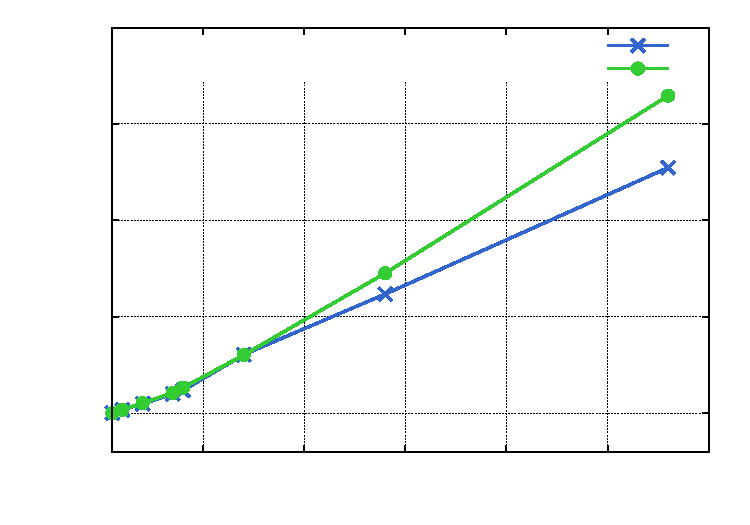
\includegraphics{plot-comp-rowCalcT_nogatherInt_all_500_4000_56_slide_2}}%
    \gplfronttext
  \end{picture}%
\endgroup
}
%%     \column{.5\textwidth}
%%     \resizebox{\columnwidth}{!}{% GNUPLOT: LaTeX picture with Postscript
\begingroup
  \makeatletter
  \providecommand\color[2][]{%
    \GenericError{(gnuplot) \space\space\space\@spaces}{%
      Package color not loaded in conjunction with
      terminal option `colourtext'%
    }{See the gnuplot documentation for explanation.%
    }{Either use 'blacktext' in gnuplot or load the package
      color.sty in LaTeX.}%
    \renewcommand\color[2][]{}%
  }%
  \providecommand\includegraphics[2][]{%
    \GenericError{(gnuplot) \space\space\space\@spaces}{%
      Package graphicx or graphics not loaded%
    }{See the gnuplot documentation for explanation.%
    }{The gnuplot epslatex terminal needs graphicx.sty or graphics.sty.}%
    \renewcommand\includegraphics[2][]{}%
  }%
  \providecommand\rotatebox[2]{#2}%
  \@ifundefined{ifGPcolor}{%
    \newif\ifGPcolor
    \GPcolortrue
  }{}%
  \@ifundefined{ifGPblacktext}{%
    \newif\ifGPblacktext
    \GPblacktextfalse
  }{}%
  % define a \g@addto@macro without @ in the name:
  \let\gplgaddtomacro\g@addto@macro
  % define empty templates for all commands taking text:
  \gdef\gplbacktext{}%
  \gdef\gplfronttext{}%
  \makeatother
  \ifGPblacktext
    % no textcolor at all
    \def\colorrgb#1{}%
    \def\colorgray#1{}%
  \else
    % gray or color?
    \ifGPcolor
      \def\colorrgb#1{\color[rgb]{#1}}%
      \def\colorgray#1{\color[gray]{#1}}%
      \expandafter\def\csname LTw\endcsname{\color{white}}%
      \expandafter\def\csname LTb\endcsname{\color{black}}%
      \expandafter\def\csname LTa\endcsname{\color{black}}%
      \expandafter\def\csname LT0\endcsname{\color[rgb]{1,0,0}}%
      \expandafter\def\csname LT1\endcsname{\color[rgb]{0,1,0}}%
      \expandafter\def\csname LT2\endcsname{\color[rgb]{0,0,1}}%
      \expandafter\def\csname LT3\endcsname{\color[rgb]{1,0,1}}%
      \expandafter\def\csname LT4\endcsname{\color[rgb]{0,1,1}}%
      \expandafter\def\csname LT5\endcsname{\color[rgb]{1,1,0}}%
      \expandafter\def\csname LT6\endcsname{\color[rgb]{0,0,0}}%
      \expandafter\def\csname LT7\endcsname{\color[rgb]{1,0.3,0}}%
      \expandafter\def\csname LT8\endcsname{\color[rgb]{0.5,0.5,0.5}}%
    \else
      % gray
      \def\colorrgb#1{\color{black}}%
      \def\colorgray#1{\color[gray]{#1}}%
      \expandafter\def\csname LTw\endcsname{\color{white}}%
      \expandafter\def\csname LTb\endcsname{\color{black}}%
      \expandafter\def\csname LTa\endcsname{\color{black}}%
      \expandafter\def\csname LT0\endcsname{\color{black}}%
      \expandafter\def\csname LT1\endcsname{\color{black}}%
      \expandafter\def\csname LT2\endcsname{\color{black}}%
      \expandafter\def\csname LT3\endcsname{\color{black}}%
      \expandafter\def\csname LT4\endcsname{\color{black}}%
      \expandafter\def\csname LT5\endcsname{\color{black}}%
      \expandafter\def\csname LT6\endcsname{\color{black}}%
      \expandafter\def\csname LT7\endcsname{\color{black}}%
      \expandafter\def\csname LT8\endcsname{\color{black}}%
    \fi
  \fi
  \setlength{\unitlength}{0.0500bp}%
  \begin{picture}(7200.00,5040.00)%
    \gplgaddtomacro\gplbacktext{%
      \csname LTb\endcsname%
      \put(946,1074){\makebox(0,0)[r]{\strut{} 1}}%
      \csname LTb\endcsname%
      \put(946,1999){\makebox(0,0)[r]{\strut{} 1.5}}%
      \csname LTb\endcsname%
      \put(946,2925){\makebox(0,0)[r]{\strut{} 2}}%
      \csname LTb\endcsname%
      \put(946,3850){\makebox(0,0)[r]{\strut{} 2.5}}%
      \csname LTb\endcsname%
      \put(946,4775){\makebox(0,0)[r]{\strut{} 3}}%
      \csname LTb\endcsname%
      \put(1951,484){\makebox(0,0){\strut{} 10}}%
      \csname LTb\endcsname%
      \put(2922,484){\makebox(0,0){\strut{} 20}}%
      \csname LTb\endcsname%
      \put(3892,484){\makebox(0,0){\strut{} 30}}%
      \csname LTb\endcsname%
      \put(4862,484){\makebox(0,0){\strut{} 40}}%
      \csname LTb\endcsname%
      \put(5833,484){\makebox(0,0){\strut{} 50}}%
      \csname LTb\endcsname%
      \put(6803,484){\makebox(0,0){\strut{} 60}}%
      \put(176,2739){\rotatebox{-270}{\makebox(0,0){\strut{}$T_{\textrm{row}}^{\phantom{row}(n)} / T_{\textrm{row}}^{\phantom{row}(1)}$}}}%
      \put(3940,154){\makebox(0,0){\strut{}$n$ parallel degree}}%
    }%
    \gplgaddtomacro\gplfronttext{%
      \csname LTb\endcsname%
      \put(5698,4602){\makebox(0,0)[r]{\strut{}uso della Rete di Interconnessione}}%
      \csname LTb\endcsname%
      \put(5698,4382){\makebox(0,0)[r]{\strut{}uso della Memoria Condivisa}}%
    }%
    \gplbacktext
    \put(0,0){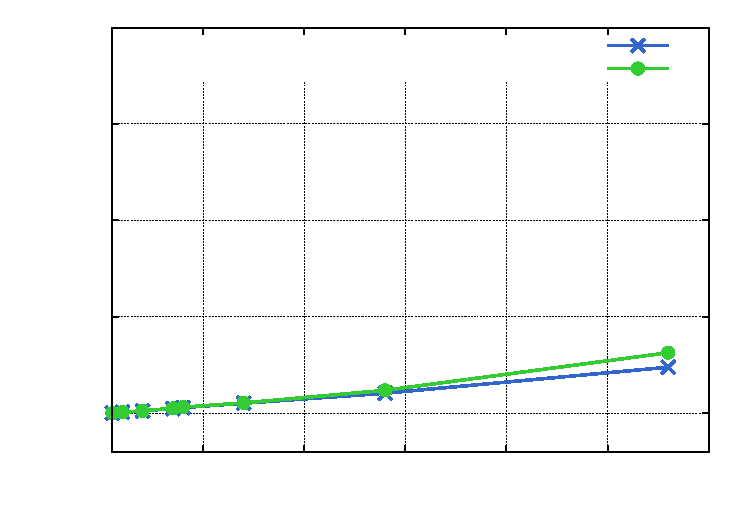
\includegraphics{plot-comp-rowCalcT_nogatherFloat_all_500_4000_56_slide_2}}%
    \gplfronttext
  \end{picture}%
\endgroup
}
%%   \end{columns}
%% \end{frame}


%% \begin{frame}
%%   \frametitle{Confronto}
%%   \begin{columns}
%%   \column{.33\textwidth}
%%   {\small matrice 56x56}
%%   \column{.33\textwidth}
%%   {\small matrice 168x168}
%%   \column{.33\textwidth}
%%   {\small matrice 280x280}
%%   \end{columns}
%%   \vspace{5mm}
%%   \begin{columns}[c]
%%   \column{.33\textwidth}
%%   \resizebox{\columnwidth}{!}{% GNUPLOT: LaTeX picture with Postscript
\begingroup
  \makeatletter
  \providecommand\color[2][]{%
    \GenericError{(gnuplot) \space\space\space\@spaces}{%
      Package color not loaded in conjunction with
      terminal option `colourtext'%
    }{See the gnuplot documentation for explanation.%
    }{Either use 'blacktext' in gnuplot or load the package
      color.sty in LaTeX.}%
    \renewcommand\color[2][]{}%
  }%
  \providecommand\includegraphics[2][]{%
    \GenericError{(gnuplot) \space\space\space\@spaces}{%
      Package graphicx or graphics not loaded%
    }{See the gnuplot documentation for explanation.%
    }{The gnuplot epslatex terminal needs graphicx.sty or graphics.sty.}%
    \renewcommand\includegraphics[2][]{}%
  }%
  \providecommand\rotatebox[2]{#2}%
  \@ifundefined{ifGPcolor}{%
    \newif\ifGPcolor
    \GPcolortrue
  }{}%
  \@ifundefined{ifGPblacktext}{%
    \newif\ifGPblacktext
    \GPblacktextfalse
  }{}%
  % define a \g@addto@macro without @ in the name:
  \let\gplgaddtomacro\g@addto@macro
  % define empty templates for all commands taking text:
  \gdef\gplbacktext{}%
  \gdef\gplfronttext{}%
  \makeatother
  \ifGPblacktext
    % no textcolor at all
    \def\colorrgb#1{}%
    \def\colorgray#1{}%
  \else
    % gray or color?
    \ifGPcolor
      \def\colorrgb#1{\color[rgb]{#1}}%
      \def\colorgray#1{\color[gray]{#1}}%
      \expandafter\def\csname LTw\endcsname{\color{white}}%
      \expandafter\def\csname LTb\endcsname{\color{black}}%
      \expandafter\def\csname LTa\endcsname{\color{black}}%
      \expandafter\def\csname LT0\endcsname{\color[rgb]{1,0,0}}%
      \expandafter\def\csname LT1\endcsname{\color[rgb]{0,1,0}}%
      \expandafter\def\csname LT2\endcsname{\color[rgb]{0,0,1}}%
      \expandafter\def\csname LT3\endcsname{\color[rgb]{1,0,1}}%
      \expandafter\def\csname LT4\endcsname{\color[rgb]{0,1,1}}%
      \expandafter\def\csname LT5\endcsname{\color[rgb]{1,1,0}}%
      \expandafter\def\csname LT6\endcsname{\color[rgb]{0,0,0}}%
      \expandafter\def\csname LT7\endcsname{\color[rgb]{1,0.3,0}}%
      \expandafter\def\csname LT8\endcsname{\color[rgb]{0.5,0.5,0.5}}%
    \else
      % gray
      \def\colorrgb#1{\color{black}}%
      \def\colorgray#1{\color[gray]{#1}}%
      \expandafter\def\csname LTw\endcsname{\color{white}}%
      \expandafter\def\csname LTb\endcsname{\color{black}}%
      \expandafter\def\csname LTa\endcsname{\color{black}}%
      \expandafter\def\csname LT0\endcsname{\color{black}}%
      \expandafter\def\csname LT1\endcsname{\color{black}}%
      \expandafter\def\csname LT2\endcsname{\color{black}}%
      \expandafter\def\csname LT3\endcsname{\color{black}}%
      \expandafter\def\csname LT4\endcsname{\color{black}}%
      \expandafter\def\csname LT5\endcsname{\color{black}}%
      \expandafter\def\csname LT6\endcsname{\color{black}}%
      \expandafter\def\csname LT7\endcsname{\color{black}}%
      \expandafter\def\csname LT8\endcsname{\color{black}}%
    \fi
  \fi
  \setlength{\unitlength}{0.0500bp}%
  \begin{picture}(7200.00,5040.00)%
    \gplgaddtomacro\gplbacktext{%
      \csname LTb\endcsname%
      \put(946,1074){\makebox(0,0)[r]{\strut{} 1}}%
      \csname LTb\endcsname%
      \put(946,1999){\makebox(0,0)[r]{\strut{} 1.5}}%
      \csname LTb\endcsname%
      \put(946,2925){\makebox(0,0)[r]{\strut{} 2}}%
      \csname LTb\endcsname%
      \put(946,3850){\makebox(0,0)[r]{\strut{} 2.5}}%
      \csname LTb\endcsname%
      \put(946,4775){\makebox(0,0)[r]{\strut{} 3}}%
      \csname LTb\endcsname%
      \put(1951,484){\makebox(0,0){\strut{} 10}}%
      \csname LTb\endcsname%
      \put(2922,484){\makebox(0,0){\strut{} 20}}%
      \csname LTb\endcsname%
      \put(3892,484){\makebox(0,0){\strut{} 30}}%
      \csname LTb\endcsname%
      \put(4862,484){\makebox(0,0){\strut{} 40}}%
      \csname LTb\endcsname%
      \put(5833,484){\makebox(0,0){\strut{} 50}}%
      \csname LTb\endcsname%
      \put(6803,484){\makebox(0,0){\strut{} 60}}%
      \put(176,2739){\rotatebox{-270}{\makebox(0,0){\strut{}$T_{\textrm{row}}^{\phantom{row}(n)} / T_{\textrm{row}}^{\phantom{row}(1)}$}}}%
      \put(3940,154){\makebox(0,0){\strut{}$n$ parallel degree}}%
    }%
    \gplgaddtomacro\gplfronttext{%
      \csname LTb\endcsname%
      \put(5698,4602){\makebox(0,0)[r]{\strut{}uso della Rete di Interconnessione}}%
      \csname LTb\endcsname%
      \put(5698,4382){\makebox(0,0)[r]{\strut{}uso della Memoria Condivisa}}%
    }%
    \gplbacktext
    \put(0,0){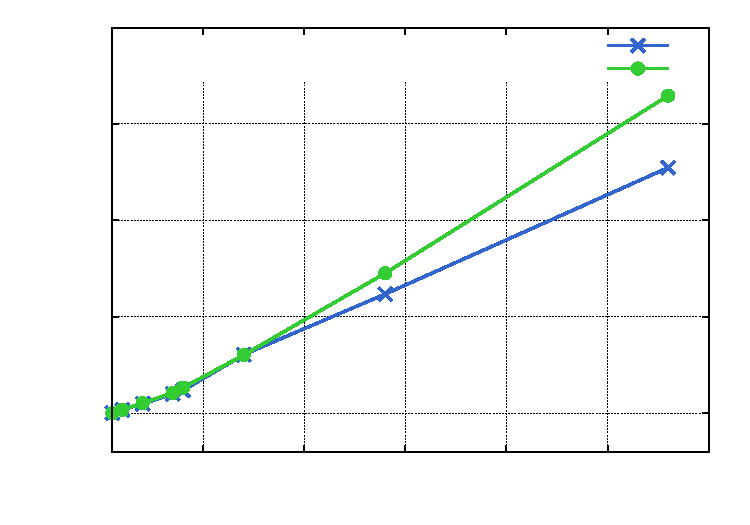
\includegraphics{plot-comp-rowCalcT_nogatherInt_all_500_4000_56_slide_2}}%
    \gplfronttext
  \end{picture}%
\endgroup
}
%%   \column{.33\textwidth}
%%   \resizebox{\columnwidth}{!}{% GNUPLOT: LaTeX picture with Postscript
\begingroup
  \makeatletter
  \providecommand\color[2][]{%
    \GenericError{(gnuplot) \space\space\space\@spaces}{%
      Package color not loaded in conjunction with
      terminal option `colourtext'%
    }{See the gnuplot documentation for explanation.%
    }{Either use 'blacktext' in gnuplot or load the package
      color.sty in LaTeX.}%
    \renewcommand\color[2][]{}%
  }%
  \providecommand\includegraphics[2][]{%
    \GenericError{(gnuplot) \space\space\space\@spaces}{%
      Package graphicx or graphics not loaded%
    }{See the gnuplot documentation for explanation.%
    }{The gnuplot epslatex terminal needs graphicx.sty or graphics.sty.}%
    \renewcommand\includegraphics[2][]{}%
  }%
  \providecommand\rotatebox[2]{#2}%
  \@ifundefined{ifGPcolor}{%
    \newif\ifGPcolor
    \GPcolortrue
  }{}%
  \@ifundefined{ifGPblacktext}{%
    \newif\ifGPblacktext
    \GPblacktextfalse
  }{}%
  % define a \g@addto@macro without @ in the name:
  \let\gplgaddtomacro\g@addto@macro
  % define empty templates for all commands taking text:
  \gdef\gplbacktext{}%
  \gdef\gplfronttext{}%
  \makeatother
  \ifGPblacktext
    % no textcolor at all
    \def\colorrgb#1{}%
    \def\colorgray#1{}%
  \else
    % gray or color?
    \ifGPcolor
      \def\colorrgb#1{\color[rgb]{#1}}%
      \def\colorgray#1{\color[gray]{#1}}%
      \expandafter\def\csname LTw\endcsname{\color{white}}%
      \expandafter\def\csname LTb\endcsname{\color{black}}%
      \expandafter\def\csname LTa\endcsname{\color{black}}%
      \expandafter\def\csname LT0\endcsname{\color[rgb]{1,0,0}}%
      \expandafter\def\csname LT1\endcsname{\color[rgb]{0,1,0}}%
      \expandafter\def\csname LT2\endcsname{\color[rgb]{0,0,1}}%
      \expandafter\def\csname LT3\endcsname{\color[rgb]{1,0,1}}%
      \expandafter\def\csname LT4\endcsname{\color[rgb]{0,1,1}}%
      \expandafter\def\csname LT5\endcsname{\color[rgb]{1,1,0}}%
      \expandafter\def\csname LT6\endcsname{\color[rgb]{0,0,0}}%
      \expandafter\def\csname LT7\endcsname{\color[rgb]{1,0.3,0}}%
      \expandafter\def\csname LT8\endcsname{\color[rgb]{0.5,0.5,0.5}}%
    \else
      % gray
      \def\colorrgb#1{\color{black}}%
      \def\colorgray#1{\color[gray]{#1}}%
      \expandafter\def\csname LTw\endcsname{\color{white}}%
      \expandafter\def\csname LTb\endcsname{\color{black}}%
      \expandafter\def\csname LTa\endcsname{\color{black}}%
      \expandafter\def\csname LT0\endcsname{\color{black}}%
      \expandafter\def\csname LT1\endcsname{\color{black}}%
      \expandafter\def\csname LT2\endcsname{\color{black}}%
      \expandafter\def\csname LT3\endcsname{\color{black}}%
      \expandafter\def\csname LT4\endcsname{\color{black}}%
      \expandafter\def\csname LT5\endcsname{\color{black}}%
      \expandafter\def\csname LT6\endcsname{\color{black}}%
      \expandafter\def\csname LT7\endcsname{\color{black}}%
      \expandafter\def\csname LT8\endcsname{\color{black}}%
    \fi
  \fi
  \setlength{\unitlength}{0.0500bp}%
  \begin{picture}(7200.00,5040.00)%
    \gplgaddtomacro\gplbacktext{%
      \csname LTb\endcsname%
      \put(946,1074){\makebox(0,0)[r]{\strut{} 1}}%
      \csname LTb\endcsname%
      \put(946,1999){\makebox(0,0)[r]{\strut{} 1.5}}%
      \csname LTb\endcsname%
      \put(946,2925){\makebox(0,0)[r]{\strut{} 2}}%
      \csname LTb\endcsname%
      \put(946,3850){\makebox(0,0)[r]{\strut{} 2.5}}%
      \csname LTb\endcsname%
      \put(946,4775){\makebox(0,0)[r]{\strut{} 3}}%
      \csname LTb\endcsname%
      \put(1951,484){\makebox(0,0){\strut{} 10}}%
      \csname LTb\endcsname%
      \put(2922,484){\makebox(0,0){\strut{} 20}}%
      \csname LTb\endcsname%
      \put(3892,484){\makebox(0,0){\strut{} 30}}%
      \csname LTb\endcsname%
      \put(4862,484){\makebox(0,0){\strut{} 40}}%
      \csname LTb\endcsname%
      \put(5833,484){\makebox(0,0){\strut{} 50}}%
      \csname LTb\endcsname%
      \put(6803,484){\makebox(0,0){\strut{} 60}}%
      \put(176,2739){\rotatebox{-270}{\makebox(0,0){\strut{}$T_{\textrm{row}}^{\phantom{row}(n)} / T_{\textrm{row}}^{\phantom{row}(1)}$}}}%
      \put(3940,154){\makebox(0,0){\strut{}$n$ parallel degree}}%
    }%
    \gplgaddtomacro\gplfronttext{%
      \csname LTb\endcsname%
      \put(5698,4602){\makebox(0,0)[r]{\strut{}uso della Rete di Interconnessione}}%
      \csname LTb\endcsname%
      \put(5698,4382){\makebox(0,0)[r]{\strut{}uso della Memoria Condivisa}}%
    }%
    \gplbacktext
    \put(0,0){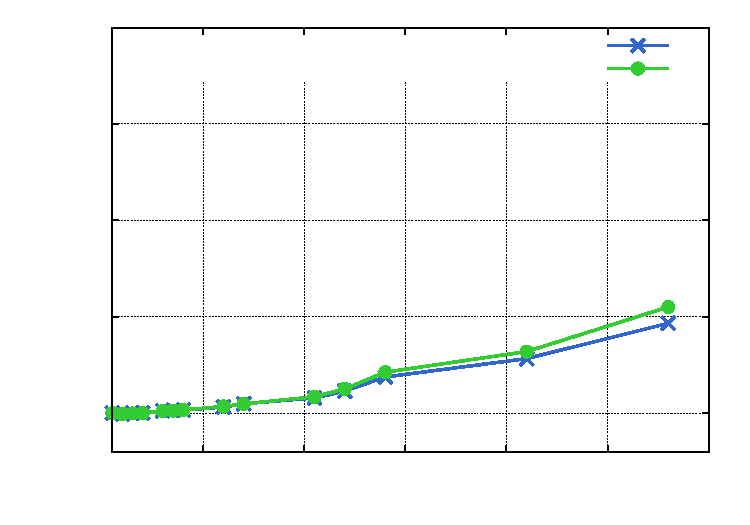
\includegraphics{plot-comp-rowCalcT_nogatherInt_all_500_4000_168_slide_2}}%
    \gplfronttext
  \end{picture}%
\endgroup
}
%%   \column{.33\textwidth}
%%   \resizebox{\columnwidth}{!}{% GNUPLOT: LaTeX picture with Postscript
\begingroup
  \makeatletter
  \providecommand\color[2][]{%
    \GenericError{(gnuplot) \space\space\space\@spaces}{%
      Package color not loaded in conjunction with
      terminal option `colourtext'%
    }{See the gnuplot documentation for explanation.%
    }{Either use 'blacktext' in gnuplot or load the package
      color.sty in LaTeX.}%
    \renewcommand\color[2][]{}%
  }%
  \providecommand\includegraphics[2][]{%
    \GenericError{(gnuplot) \space\space\space\@spaces}{%
      Package graphicx or graphics not loaded%
    }{See the gnuplot documentation for explanation.%
    }{The gnuplot epslatex terminal needs graphicx.sty or graphics.sty.}%
    \renewcommand\includegraphics[2][]{}%
  }%
  \providecommand\rotatebox[2]{#2}%
  \@ifundefined{ifGPcolor}{%
    \newif\ifGPcolor
    \GPcolortrue
  }{}%
  \@ifundefined{ifGPblacktext}{%
    \newif\ifGPblacktext
    \GPblacktextfalse
  }{}%
  % define a \g@addto@macro without @ in the name:
  \let\gplgaddtomacro\g@addto@macro
  % define empty templates for all commands taking text:
  \gdef\gplbacktext{}%
  \gdef\gplfronttext{}%
  \makeatother
  \ifGPblacktext
    % no textcolor at all
    \def\colorrgb#1{}%
    \def\colorgray#1{}%
  \else
    % gray or color?
    \ifGPcolor
      \def\colorrgb#1{\color[rgb]{#1}}%
      \def\colorgray#1{\color[gray]{#1}}%
      \expandafter\def\csname LTw\endcsname{\color{white}}%
      \expandafter\def\csname LTb\endcsname{\color{black}}%
      \expandafter\def\csname LTa\endcsname{\color{black}}%
      \expandafter\def\csname LT0\endcsname{\color[rgb]{1,0,0}}%
      \expandafter\def\csname LT1\endcsname{\color[rgb]{0,1,0}}%
      \expandafter\def\csname LT2\endcsname{\color[rgb]{0,0,1}}%
      \expandafter\def\csname LT3\endcsname{\color[rgb]{1,0,1}}%
      \expandafter\def\csname LT4\endcsname{\color[rgb]{0,1,1}}%
      \expandafter\def\csname LT5\endcsname{\color[rgb]{1,1,0}}%
      \expandafter\def\csname LT6\endcsname{\color[rgb]{0,0,0}}%
      \expandafter\def\csname LT7\endcsname{\color[rgb]{1,0.3,0}}%
      \expandafter\def\csname LT8\endcsname{\color[rgb]{0.5,0.5,0.5}}%
    \else
      % gray
      \def\colorrgb#1{\color{black}}%
      \def\colorgray#1{\color[gray]{#1}}%
      \expandafter\def\csname LTw\endcsname{\color{white}}%
      \expandafter\def\csname LTb\endcsname{\color{black}}%
      \expandafter\def\csname LTa\endcsname{\color{black}}%
      \expandafter\def\csname LT0\endcsname{\color{black}}%
      \expandafter\def\csname LT1\endcsname{\color{black}}%
      \expandafter\def\csname LT2\endcsname{\color{black}}%
      \expandafter\def\csname LT3\endcsname{\color{black}}%
      \expandafter\def\csname LT4\endcsname{\color{black}}%
      \expandafter\def\csname LT5\endcsname{\color{black}}%
      \expandafter\def\csname LT6\endcsname{\color{black}}%
      \expandafter\def\csname LT7\endcsname{\color{black}}%
      \expandafter\def\csname LT8\endcsname{\color{black}}%
    \fi
  \fi
  \setlength{\unitlength}{0.0500bp}%
  \begin{picture}(7200.00,5040.00)%
    \gplgaddtomacro\gplbacktext{%
      \csname LTb\endcsname%
      \put(946,1074){\makebox(0,0)[r]{\strut{} 1}}%
      \csname LTb\endcsname%
      \put(946,1999){\makebox(0,0)[r]{\strut{} 1.5}}%
      \csname LTb\endcsname%
      \put(946,2925){\makebox(0,0)[r]{\strut{} 2}}%
      \csname LTb\endcsname%
      \put(946,3850){\makebox(0,0)[r]{\strut{} 2.5}}%
      \csname LTb\endcsname%
      \put(946,4775){\makebox(0,0)[r]{\strut{} 3}}%
      \csname LTb\endcsname%
      \put(1951,484){\makebox(0,0){\strut{} 10}}%
      \csname LTb\endcsname%
      \put(2922,484){\makebox(0,0){\strut{} 20}}%
      \csname LTb\endcsname%
      \put(3892,484){\makebox(0,0){\strut{} 30}}%
      \csname LTb\endcsname%
      \put(4862,484){\makebox(0,0){\strut{} 40}}%
      \csname LTb\endcsname%
      \put(5833,484){\makebox(0,0){\strut{} 50}}%
      \csname LTb\endcsname%
      \put(6803,484){\makebox(0,0){\strut{} 60}}%
      \put(176,2739){\rotatebox{-270}{\makebox(0,0){\strut{}$T_{\textrm{row}}^{\phantom{row}(n)} / T_{\textrm{row}}^{\phantom{row}(1)}$}}}%
      \put(3940,154){\makebox(0,0){\strut{}$n$ parallel degree}}%
    }%
    \gplgaddtomacro\gplfronttext{%
      \csname LTb\endcsname%
      \put(5698,4602){\makebox(0,0)[r]{\strut{}uso della Rete di Interconnessione}}%
      \csname LTb\endcsname%
      \put(5698,4382){\makebox(0,0)[r]{\strut{}uso della Memoria Condivisa}}%
    }%
    \gplbacktext
    \put(0,0){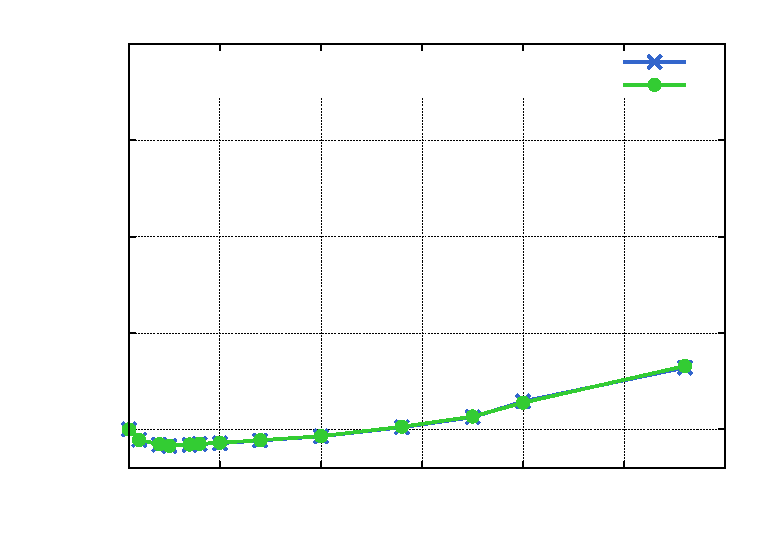
\includegraphics{plot-comp-rowCalcT_nogatherInt_all_500_4000_280_slide_2}}%
    \gplfronttext
  \end{picture}%
\endgroup
}
%%   \end{columns}
%%   \begin{columns}[c]
%%   \column{.33\textwidth}
%%   \resizebox{\columnwidth}{!}{% GNUPLOT: LaTeX picture with Postscript
\begingroup
  \makeatletter
  \providecommand\color[2][]{%
    \GenericError{(gnuplot) \space\space\space\@spaces}{%
      Package color not loaded in conjunction with
      terminal option `colourtext'%
    }{See the gnuplot documentation for explanation.%
    }{Either use 'blacktext' in gnuplot or load the package
      color.sty in LaTeX.}%
    \renewcommand\color[2][]{}%
  }%
  \providecommand\includegraphics[2][]{%
    \GenericError{(gnuplot) \space\space\space\@spaces}{%
      Package graphicx or graphics not loaded%
    }{See the gnuplot documentation for explanation.%
    }{The gnuplot epslatex terminal needs graphicx.sty or graphics.sty.}%
    \renewcommand\includegraphics[2][]{}%
  }%
  \providecommand\rotatebox[2]{#2}%
  \@ifundefined{ifGPcolor}{%
    \newif\ifGPcolor
    \GPcolortrue
  }{}%
  \@ifundefined{ifGPblacktext}{%
    \newif\ifGPblacktext
    \GPblacktextfalse
  }{}%
  % define a \g@addto@macro without @ in the name:
  \let\gplgaddtomacro\g@addto@macro
  % define empty templates for all commands taking text:
  \gdef\gplbacktext{}%
  \gdef\gplfronttext{}%
  \makeatother
  \ifGPblacktext
    % no textcolor at all
    \def\colorrgb#1{}%
    \def\colorgray#1{}%
  \else
    % gray or color?
    \ifGPcolor
      \def\colorrgb#1{\color[rgb]{#1}}%
      \def\colorgray#1{\color[gray]{#1}}%
      \expandafter\def\csname LTw\endcsname{\color{white}}%
      \expandafter\def\csname LTb\endcsname{\color{black}}%
      \expandafter\def\csname LTa\endcsname{\color{black}}%
      \expandafter\def\csname LT0\endcsname{\color[rgb]{1,0,0}}%
      \expandafter\def\csname LT1\endcsname{\color[rgb]{0,1,0}}%
      \expandafter\def\csname LT2\endcsname{\color[rgb]{0,0,1}}%
      \expandafter\def\csname LT3\endcsname{\color[rgb]{1,0,1}}%
      \expandafter\def\csname LT4\endcsname{\color[rgb]{0,1,1}}%
      \expandafter\def\csname LT5\endcsname{\color[rgb]{1,1,0}}%
      \expandafter\def\csname LT6\endcsname{\color[rgb]{0,0,0}}%
      \expandafter\def\csname LT7\endcsname{\color[rgb]{1,0.3,0}}%
      \expandafter\def\csname LT8\endcsname{\color[rgb]{0.5,0.5,0.5}}%
    \else
      % gray
      \def\colorrgb#1{\color{black}}%
      \def\colorgray#1{\color[gray]{#1}}%
      \expandafter\def\csname LTw\endcsname{\color{white}}%
      \expandafter\def\csname LTb\endcsname{\color{black}}%
      \expandafter\def\csname LTa\endcsname{\color{black}}%
      \expandafter\def\csname LT0\endcsname{\color{black}}%
      \expandafter\def\csname LT1\endcsname{\color{black}}%
      \expandafter\def\csname LT2\endcsname{\color{black}}%
      \expandafter\def\csname LT3\endcsname{\color{black}}%
      \expandafter\def\csname LT4\endcsname{\color{black}}%
      \expandafter\def\csname LT5\endcsname{\color{black}}%
      \expandafter\def\csname LT6\endcsname{\color{black}}%
      \expandafter\def\csname LT7\endcsname{\color{black}}%
      \expandafter\def\csname LT8\endcsname{\color{black}}%
    \fi
  \fi
  \setlength{\unitlength}{0.0500bp}%
  \begin{picture}(7200.00,5040.00)%
    \gplgaddtomacro\gplbacktext{%
      \csname LTb\endcsname%
      \put(946,1074){\makebox(0,0)[r]{\strut{} 1}}%
      \csname LTb\endcsname%
      \put(946,1999){\makebox(0,0)[r]{\strut{} 1.5}}%
      \csname LTb\endcsname%
      \put(946,2925){\makebox(0,0)[r]{\strut{} 2}}%
      \csname LTb\endcsname%
      \put(946,3850){\makebox(0,0)[r]{\strut{} 2.5}}%
      \csname LTb\endcsname%
      \put(946,4775){\makebox(0,0)[r]{\strut{} 3}}%
      \csname LTb\endcsname%
      \put(1951,484){\makebox(0,0){\strut{} 10}}%
      \csname LTb\endcsname%
      \put(2922,484){\makebox(0,0){\strut{} 20}}%
      \csname LTb\endcsname%
      \put(3892,484){\makebox(0,0){\strut{} 30}}%
      \csname LTb\endcsname%
      \put(4862,484){\makebox(0,0){\strut{} 40}}%
      \csname LTb\endcsname%
      \put(5833,484){\makebox(0,0){\strut{} 50}}%
      \csname LTb\endcsname%
      \put(6803,484){\makebox(0,0){\strut{} 60}}%
      \put(176,2739){\rotatebox{-270}{\makebox(0,0){\strut{}$T_{\textrm{row}}^{\phantom{row}(n)} / T_{\textrm{row}}^{\phantom{row}(1)}$}}}%
      \put(3940,154){\makebox(0,0){\strut{}$n$ parallel degree}}%
    }%
    \gplgaddtomacro\gplfronttext{%
      \csname LTb\endcsname%
      \put(5698,4602){\makebox(0,0)[r]{\strut{}uso della Rete di Interconnessione}}%
      \csname LTb\endcsname%
      \put(5698,4382){\makebox(0,0)[r]{\strut{}uso della Memoria Condivisa}}%
    }%
    \gplbacktext
    \put(0,0){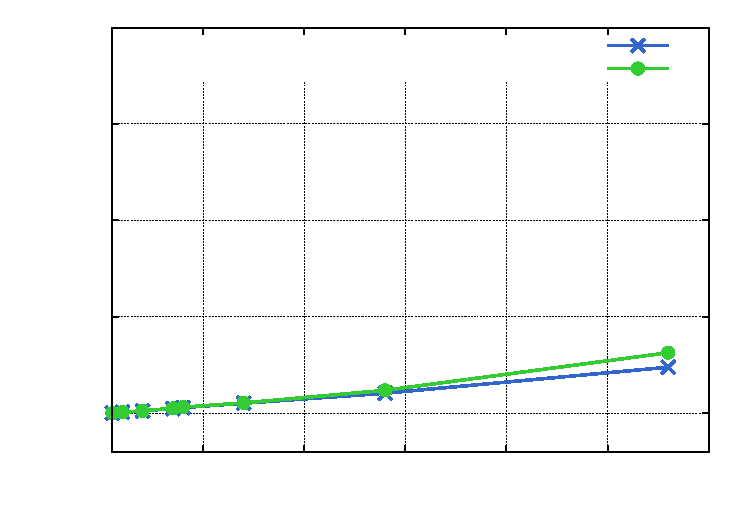
\includegraphics{plot-comp-rowCalcT_nogatherFloat_all_500_4000_56_slide_2}}%
    \gplfronttext
  \end{picture}%
\endgroup
}
%%   \column{.33\textwidth}
%%   \resizebox{\columnwidth}{!}{% GNUPLOT: LaTeX picture with Postscript
\begingroup
  \makeatletter
  \providecommand\color[2][]{%
    \GenericError{(gnuplot) \space\space\space\@spaces}{%
      Package color not loaded in conjunction with
      terminal option `colourtext'%
    }{See the gnuplot documentation for explanation.%
    }{Either use 'blacktext' in gnuplot or load the package
      color.sty in LaTeX.}%
    \renewcommand\color[2][]{}%
  }%
  \providecommand\includegraphics[2][]{%
    \GenericError{(gnuplot) \space\space\space\@spaces}{%
      Package graphicx or graphics not loaded%
    }{See the gnuplot documentation for explanation.%
    }{The gnuplot epslatex terminal needs graphicx.sty or graphics.sty.}%
    \renewcommand\includegraphics[2][]{}%
  }%
  \providecommand\rotatebox[2]{#2}%
  \@ifundefined{ifGPcolor}{%
    \newif\ifGPcolor
    \GPcolortrue
  }{}%
  \@ifundefined{ifGPblacktext}{%
    \newif\ifGPblacktext
    \GPblacktextfalse
  }{}%
  % define a \g@addto@macro without @ in the name:
  \let\gplgaddtomacro\g@addto@macro
  % define empty templates for all commands taking text:
  \gdef\gplbacktext{}%
  \gdef\gplfronttext{}%
  \makeatother
  \ifGPblacktext
    % no textcolor at all
    \def\colorrgb#1{}%
    \def\colorgray#1{}%
  \else
    % gray or color?
    \ifGPcolor
      \def\colorrgb#1{\color[rgb]{#1}}%
      \def\colorgray#1{\color[gray]{#1}}%
      \expandafter\def\csname LTw\endcsname{\color{white}}%
      \expandafter\def\csname LTb\endcsname{\color{black}}%
      \expandafter\def\csname LTa\endcsname{\color{black}}%
      \expandafter\def\csname LT0\endcsname{\color[rgb]{1,0,0}}%
      \expandafter\def\csname LT1\endcsname{\color[rgb]{0,1,0}}%
      \expandafter\def\csname LT2\endcsname{\color[rgb]{0,0,1}}%
      \expandafter\def\csname LT3\endcsname{\color[rgb]{1,0,1}}%
      \expandafter\def\csname LT4\endcsname{\color[rgb]{0,1,1}}%
      \expandafter\def\csname LT5\endcsname{\color[rgb]{1,1,0}}%
      \expandafter\def\csname LT6\endcsname{\color[rgb]{0,0,0}}%
      \expandafter\def\csname LT7\endcsname{\color[rgb]{1,0.3,0}}%
      \expandafter\def\csname LT8\endcsname{\color[rgb]{0.5,0.5,0.5}}%
    \else
      % gray
      \def\colorrgb#1{\color{black}}%
      \def\colorgray#1{\color[gray]{#1}}%
      \expandafter\def\csname LTw\endcsname{\color{white}}%
      \expandafter\def\csname LTb\endcsname{\color{black}}%
      \expandafter\def\csname LTa\endcsname{\color{black}}%
      \expandafter\def\csname LT0\endcsname{\color{black}}%
      \expandafter\def\csname LT1\endcsname{\color{black}}%
      \expandafter\def\csname LT2\endcsname{\color{black}}%
      \expandafter\def\csname LT3\endcsname{\color{black}}%
      \expandafter\def\csname LT4\endcsname{\color{black}}%
      \expandafter\def\csname LT5\endcsname{\color{black}}%
      \expandafter\def\csname LT6\endcsname{\color{black}}%
      \expandafter\def\csname LT7\endcsname{\color{black}}%
      \expandafter\def\csname LT8\endcsname{\color{black}}%
    \fi
  \fi
  \setlength{\unitlength}{0.0500bp}%
  \begin{picture}(7200.00,5040.00)%
    \gplgaddtomacro\gplbacktext{%
      \csname LTb\endcsname%
      \put(946,1074){\makebox(0,0)[r]{\strut{} 1}}%
      \csname LTb\endcsname%
      \put(946,1999){\makebox(0,0)[r]{\strut{} 1.5}}%
      \csname LTb\endcsname%
      \put(946,2925){\makebox(0,0)[r]{\strut{} 2}}%
      \csname LTb\endcsname%
      \put(946,3850){\makebox(0,0)[r]{\strut{} 2.5}}%
      \csname LTb\endcsname%
      \put(946,4775){\makebox(0,0)[r]{\strut{} 3}}%
      \csname LTb\endcsname%
      \put(1951,484){\makebox(0,0){\strut{} 10}}%
      \csname LTb\endcsname%
      \put(2922,484){\makebox(0,0){\strut{} 20}}%
      \csname LTb\endcsname%
      \put(3892,484){\makebox(0,0){\strut{} 30}}%
      \csname LTb\endcsname%
      \put(4862,484){\makebox(0,0){\strut{} 40}}%
      \csname LTb\endcsname%
      \put(5833,484){\makebox(0,0){\strut{} 50}}%
      \csname LTb\endcsname%
      \put(6803,484){\makebox(0,0){\strut{} 60}}%
      \put(176,2739){\rotatebox{-270}{\makebox(0,0){\strut{}$T_{\textrm{row}}^{\phantom{row}(n)} / T_{\textrm{row}}^{\phantom{row}(1)}$}}}%
      \put(3940,154){\makebox(0,0){\strut{}$n$ parallel degree}}%
    }%
    \gplgaddtomacro\gplfronttext{%
      \csname LTb\endcsname%
      \put(5698,4602){\makebox(0,0)[r]{\strut{}uso della Rete di Interconnessione}}%
      \csname LTb\endcsname%
      \put(5698,4382){\makebox(0,0)[r]{\strut{}uso della Memoria Condivisa}}%
    }%
    \gplbacktext
    \put(0,0){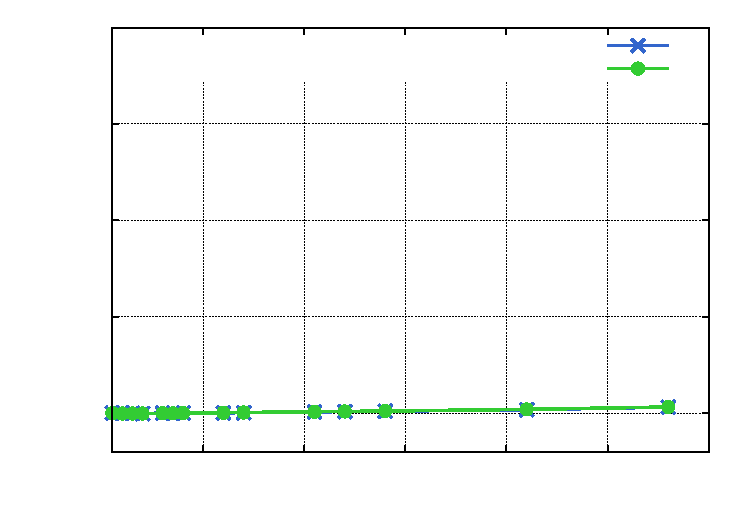
\includegraphics{plot-comp-rowCalcT_nogatherFloat_all_500_4000_168_slide_2}}%
    \gplfronttext
  \end{picture}%
\endgroup
}
%%   \column{.33\textwidth}
%%   \resizebox{\columnwidth}{!}{% GNUPLOT: LaTeX picture with Postscript
\begingroup
  \makeatletter
  \providecommand\color[2][]{%
    \GenericError{(gnuplot) \space\space\space\@spaces}{%
      Package color not loaded in conjunction with
      terminal option `colourtext'%
    }{See the gnuplot documentation for explanation.%
    }{Either use 'blacktext' in gnuplot or load the package
      color.sty in LaTeX.}%
    \renewcommand\color[2][]{}%
  }%
  \providecommand\includegraphics[2][]{%
    \GenericError{(gnuplot) \space\space\space\@spaces}{%
      Package graphicx or graphics not loaded%
    }{See the gnuplot documentation for explanation.%
    }{The gnuplot epslatex terminal needs graphicx.sty or graphics.sty.}%
    \renewcommand\includegraphics[2][]{}%
  }%
  \providecommand\rotatebox[2]{#2}%
  \@ifundefined{ifGPcolor}{%
    \newif\ifGPcolor
    \GPcolortrue
  }{}%
  \@ifundefined{ifGPblacktext}{%
    \newif\ifGPblacktext
    \GPblacktextfalse
  }{}%
  % define a \g@addto@macro without @ in the name:
  \let\gplgaddtomacro\g@addto@macro
  % define empty templates for all commands taking text:
  \gdef\gplbacktext{}%
  \gdef\gplfronttext{}%
  \makeatother
  \ifGPblacktext
    % no textcolor at all
    \def\colorrgb#1{}%
    \def\colorgray#1{}%
  \else
    % gray or color?
    \ifGPcolor
      \def\colorrgb#1{\color[rgb]{#1}}%
      \def\colorgray#1{\color[gray]{#1}}%
      \expandafter\def\csname LTw\endcsname{\color{white}}%
      \expandafter\def\csname LTb\endcsname{\color{black}}%
      \expandafter\def\csname LTa\endcsname{\color{black}}%
      \expandafter\def\csname LT0\endcsname{\color[rgb]{1,0,0}}%
      \expandafter\def\csname LT1\endcsname{\color[rgb]{0,1,0}}%
      \expandafter\def\csname LT2\endcsname{\color[rgb]{0,0,1}}%
      \expandafter\def\csname LT3\endcsname{\color[rgb]{1,0,1}}%
      \expandafter\def\csname LT4\endcsname{\color[rgb]{0,1,1}}%
      \expandafter\def\csname LT5\endcsname{\color[rgb]{1,1,0}}%
      \expandafter\def\csname LT6\endcsname{\color[rgb]{0,0,0}}%
      \expandafter\def\csname LT7\endcsname{\color[rgb]{1,0.3,0}}%
      \expandafter\def\csname LT8\endcsname{\color[rgb]{0.5,0.5,0.5}}%
    \else
      % gray
      \def\colorrgb#1{\color{black}}%
      \def\colorgray#1{\color[gray]{#1}}%
      \expandafter\def\csname LTw\endcsname{\color{white}}%
      \expandafter\def\csname LTb\endcsname{\color{black}}%
      \expandafter\def\csname LTa\endcsname{\color{black}}%
      \expandafter\def\csname LT0\endcsname{\color{black}}%
      \expandafter\def\csname LT1\endcsname{\color{black}}%
      \expandafter\def\csname LT2\endcsname{\color{black}}%
      \expandafter\def\csname LT3\endcsname{\color{black}}%
      \expandafter\def\csname LT4\endcsname{\color{black}}%
      \expandafter\def\csname LT5\endcsname{\color{black}}%
      \expandafter\def\csname LT6\endcsname{\color{black}}%
      \expandafter\def\csname LT7\endcsname{\color{black}}%
      \expandafter\def\csname LT8\endcsname{\color{black}}%
    \fi
  \fi
  \setlength{\unitlength}{0.0500bp}%
  \begin{picture}(7200.00,5040.00)%
    \gplgaddtomacro\gplbacktext{%
      \csname LTb\endcsname%
      \put(946,1074){\makebox(0,0)[r]{\strut{} 1}}%
      \csname LTb\endcsname%
      \put(946,1999){\makebox(0,0)[r]{\strut{} 1.5}}%
      \csname LTb\endcsname%
      \put(946,2925){\makebox(0,0)[r]{\strut{} 2}}%
      \csname LTb\endcsname%
      \put(946,3850){\makebox(0,0)[r]{\strut{} 2.5}}%
      \csname LTb\endcsname%
      \put(946,4775){\makebox(0,0)[r]{\strut{} 3}}%
      \csname LTb\endcsname%
      \put(1951,484){\makebox(0,0){\strut{} 10}}%
      \csname LTb\endcsname%
      \put(2922,484){\makebox(0,0){\strut{} 20}}%
      \csname LTb\endcsname%
      \put(3892,484){\makebox(0,0){\strut{} 30}}%
      \csname LTb\endcsname%
      \put(4862,484){\makebox(0,0){\strut{} 40}}%
      \csname LTb\endcsname%
      \put(5833,484){\makebox(0,0){\strut{} 50}}%
      \csname LTb\endcsname%
      \put(6803,484){\makebox(0,0){\strut{} 60}}%
      \put(176,2739){\rotatebox{-270}{\makebox(0,0){\strut{}$T_{\textrm{row}}^{\phantom{row}(n)} / T_{\textrm{row}}^{\phantom{row}(1)}$}}}%
      \put(3940,154){\makebox(0,0){\strut{}$n$ parallel degree}}%
    }%
    \gplgaddtomacro\gplfronttext{%
      \csname LTb\endcsname%
      \put(5698,4602){\makebox(0,0)[r]{\strut{}uso della Rete di Interconnessione}}%
      \csname LTb\endcsname%
      \put(5698,4382){\makebox(0,0)[r]{\strut{}uso della Memoria Condivisa}}%
    }%
    \gplbacktext
    \put(0,0){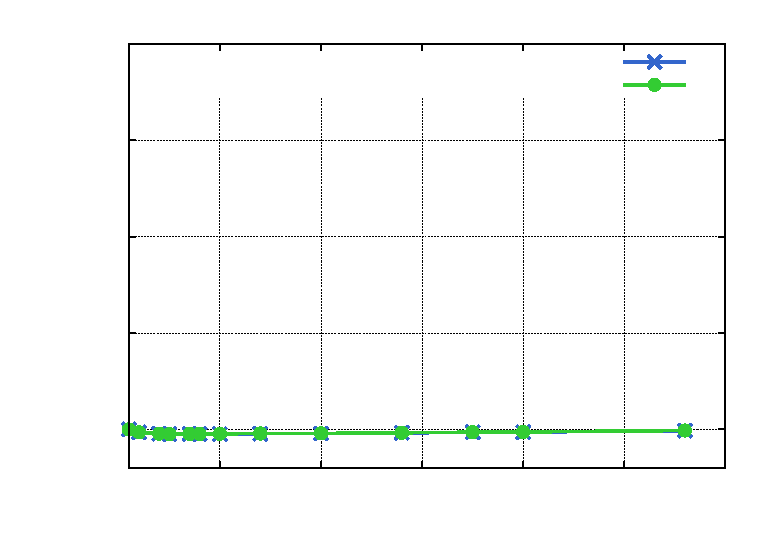
\includegraphics{plot-comp-rowCalcT_nogatherFloat_all_500_4000_280_slide_2}}%
    \gplfronttext
  \end{picture}%
\endgroup
}
%%   \end{columns}
%% \end{frame}

\begin{frame}
  \frametitle{Conclusioni}
  Si \`e quindi realizzato un supporto alle comunicazioni con due diversi approcci:
  \begin{itemize}
  \item uso della rete di interconnessione tra core
  \item uso della memoria condivisa
  \end{itemize}
  \vspace{4mm}
  Dagli esperimenti effettuati si \`e concluso:
  \begin{itemize}
  \item riduzione della latenza di comunicazione con la rete di interconnessione rispetto al caso ottimale con la memoria condivisa
  \item miglioramento del tempo di servizio in un'applicazione reale (prodotto matrice-vettore)
  \end{itemize}
\end{frame}

\begin{frame}
  \frametitle{}
  \vspace{.8cm}
  \begin{center}
    Grazie per l'attenzione.
  \end{center}
\end{frame}

\end{document}

